\documentclass[oneside, 12pt]{scrbook}

\usepackage[autooneside]{scrpage2}
\usepackage[pdftex]{graphicx}
\usepackage{mathrsfs, nicefrac, amsmath, amssymb, array, cite, float}
\usepackage{geometry}
\geometry{a4paper, left=40mm, right=25mm, top=25mm, bottom=25mm}
\usepackage{datetime}

\usepackage{sidecap}
\usepackage{afterpage}
\usepackage{subfigure}

\usepackage[format=plain,labelsep=period,labelfont=bf,font={small,onehalfspacing},textfont=sl, width=.9\textwidth]{caption}
\usepackage{setspace}
\onehalfspacing
\setlength{\parindent}{0pt} 
\setlength{\parskip}{2ex}
\bibliographystyle{apalike}

%\usepackage{titlesec}
%\titleformat{\chapter}[block]{\Large\bfseries}{\thechapter}{0.5ex}{\vspace{1ex}}{\vspace{-0.5ex}}


\pagestyle{scrheadings}
\ihead{}
\chead{}
\ohead[]{\headmark}
\cfoot[]{}
\ofoot[\pagemark]{\pagemark}

\title{Quantitative three-dimensional imaging in cancer research using optical computed tomography}
\author{Ciara McErlean}
\date{\today}
%\titlehead{A Thesis submitted for the degree of Doctor of Philosophy}
%\publishers{School of Something\\University of Somewhere}


\includeonly{methods}

\begin{document}
	\rmfamily
	%\maketitle
    %\tableofcontents
	%\listoffigures
	%\listoftables
	
%	\chapter{Acknowledgements}
%	I would like to thank my supervisor, Professor Someone. This
%	research was funded by the Imaginary Research Council.
%	\chapter{Abstract}
%	Standard 2-D microscopy has a vital role in cancer research. However, errors associated with taking 2-D samples from often heterogeneous 3-D tissues means that quantitative measurements can be unreliable. There are many examples of when having a 3-D dataset using optical contrast would be of significant interest. I have illustrated several of these areas in this thesis, using a relatively new 3-D imaging modality to investigate 3-D radiation dosimetry, quantification of drug toxicity effects and characterisation of tumour vasculature.  
%	
%	Optical computed tomography (CT) is a high-resolution 3-D imaging technique. The many existing well-characterised forms of optical contrast give optical CT an advantage over non-optical techniques such as x-ray $\mu$CT. Compared to other optical 3-D modalities, such as confocal microscopy, optical CT has the advantage of better penetration depth, after a process of optical clearing, and the ability to deliver quantitative images not simply `pretty pictures'.
%	
%	One area where 3-D information is increasingly vital, as treatments become more complex, is radiotherapy dosimetry. Microbeam radiation therapy (MRT) is an emerging form of radiotherapy using very small beams (50$\mu$m). I have shown potential of optical CT as a quality assurance method for MRT in future clinical trials and demonstrated the first 3-D visualisation of an MRT treatment. 
%	
%	Drug toxicity is of major concern during drug development and having fast, reliable and automated measures of toxicity would be beneficial. I have demonstrated the ability of optical CT to detect off-target toxicity effects in murine spleen. 3-D textural analysis produced several possible candidates of quantitative measures of toxicity, which are more reliable than 2-D measures.
%	
%	The development of tumour vasculature and its response to therapy is of significant interest in the field of cancer research. I have shown the potential for using optical CT to image murine vasculature in both the kidney and allograft neuroblastoma tumours using passive India Ink contrast. The results from optical CT can be compared to lower resolution in vivo techniques including MRI. 
	
	% A glossary and list of acronyms may go here
	% or may go in the back matter.
	
	\chapter{Introduction}

	\section{Introduction}
	\label{sec:intro}
	
	Multiparametric imaging is very important in cancer imaging. It allows the cross-correlation of observations at tumour level and  validation of new biomarkers against an established standard \cite{Padhani:2010hfa}. 
	%This is the goal for combined MRI and OptCT imaging of tumours. 
	Traditionally, tumour imaging has been approached from opposite ends of the resolution spectrum. Histology, using optical microscopy,  images tumour cells with resolution in the micron range. However, lengthy preparation steps and sectioning means that 3-D information is lost and \textit{in vivo} imaging is not possible. Magnetic resonance imaging (MRI) gives excellent visualisations of whole tumours \textit{in vivo} with contrast sensitive to malignant and benign tumours. However, the best resolution is of the order 100 microns so single cells cannot be resolved. This means the biological origin of contrast in MR images is not fully understood. 
	
	Optical computed tomography (OptCT) is a relatively new imaging modality which has the potential to bridge the gap between histology and MRI. It is the optical equivalent of x-ray CT, using mathematical reconstruction to produce cross-sectional images from projections through a sample. Samples can include embryos, tumours and entire excised tumours. The important advantage of using OptCT is its ability to give high resolution, high contrast images using optical dyes and stains common in histology. This distinguishes it from other modalities such as $\mu$-MRI.
	
	Forms of OptCT have been reported as far back as 1983 \cite{ray1983laser,kawata1990laser} %but only one projection image was used.  
	and a system similar to modern approaches was reported by Brown in 1992 \cite{Brown:1992}. 
	%A key point is the use of matching fluid  and sample clarification.
	%ncleared a sample of stained cochlea in 3BB:5MS. 600nm illumination to reduce scatter. 1.92mm radius imaged with resolution 16$\mu$m. But Brown is not referenced by either Gore or Sharpe. :(
	However, the field of OptCT has only significantly  progressed recently, starting in 1996 with Gore in the area of dosimetry  \cite{Gore:1999tg}. Later Sharpe developed a similar system in the area of biomedical microscopy, calling his technique optical projection tomography (OPT)  \cite{Sharpe:2002jp}. The availability of reasonably priced cameras and more computer power has meant that OptCT systems can be built relatively cheaply. This is yet another advantage over MRI scanners which are very expensive and time consuming to use.
	
	Having the ability to co-register MR images with high resolution, unsectioned optical images  is of significant  interest in cancer research. Understanding the origin of MR contrast on a cellular level would give MR the potential to be used more effectively in screening potential new drugs. OptCT also offers the chance to monitor tumour development in 3-D with fluorescent markers. These developments could be of significant help  in cancer imaging and treatment.
	
	
	%From meeting 13/12/12: mention problem with MR, fundamental limit on resolution, diffusion limit on protons. SNR. See papers by Paul Glover, Nottingham (micropscopy + limits of MR)
	
	
	
	%\newpage
	\section{Theory}
	\label{sec:theory}
	
	%The theory behind CT reconstruction is broadly the same between x-ray CT and OptCT. One minor difference is that it is common in x-ray CT for the detectors to rotate around the sample whereas in OptCT the sample rotates and the detectors are stationary. This introduces a minus sign at one stage of the reconstruction algorithm. [WHY IS THIS?]
	
	
	
	\subsection{Radon Space}
	
	When light passes through a substance, it is assumed to be attenuated by some small amount of intensity $\Delta I$ over a small distance $\Delta y$ 
	\begin{equation}
	\dfrac{\Delta I}{I} = -\mu(y)\Delta y
	\end{equation}
	where $\mu(y)$ is the linear attenuation coefficient.
	Taking the infinitesimal limit and integrating, 
	\begin{equation}
	\int_{I_0}^{I} \frac{1}{I}\, \mathrm{d}I = - \int_L \mu(y)\, \mathrm{d}y
	\end{equation}
	this leads to Beer's Law 
	\begin{equation}
	I(y) = I_{o}(y)\mathrm{e}^{-\int_L \mu(y)\, \mathrm{d}y}
	\label{eq:Beer}
	\end{equation}
	where $I_0$ is the intensity with no attenuation and $I(y)$ is the intensity at depth $y$. $L$ is the path the light ray has followed. The integral in the exponential term of Beer's Law takes into account the differences in attenuation coefficient along the path $L$. 
	
	From equation~(\ref{eq:Beer}) it is apparent that  the  intensity of a light beam after passing through a sample gives information about the line integral of the function $\mu$  along the line $L$. The CT scanning process records this information for many lines $L$ at different lateral positions and it is from this information that we reconstruct a map of $\mu$. \cite{natterer2001mathematics}
	The Radon transform maps a function into a set of its line integrals. Therefore, CT reconstruction involves an inverse Radon transform.
	
	
	
	To build  a 2-D map of attenuation coefficients, line integrals must be measured from multiple angles (see Figure~\ref{fig:projection}). If the sample rotates by some angle $\phi$ then the attenuation seen at position $(x, y)$  changes.
	The Radon transform, often called a projection or a view, is defined as
	\begin{equation}
	P_{\phi}(x) = \int\limits_{sample} \mu(x',y')\, \mathrm{d}y = -\ln\left(\frac{I_{\phi}(x)}{I_0}\right)
	\end{equation}
	where 
	\begin{equation}
	\begin{aligned}
	x' = x\cos\phi + y\sin\phi \\
	y' = -x\sin\phi + y\cos\phi
	\end{aligned}
	\end{equation}
	
	The projection information is stored in what is known as `Radon space' with dimensions $(x, \phi)$. Radon space is filled by measuring the projection value for all combinations of $x$ and $\phi$. A filled Radon space diagram is often referred to as a sinogram (see Figure~\ref{fig:sinogram}).
	
	In practice, the finite number of lines $L$ limits the resolution of reconstructions. There are two geometries for 2-D reconstructions; parallel beam and fan beam. The choice of scanning geometry also affects the resolution. \cite{natterer2001mathematics}
	
	\begin{figure}[H]
		\centering
		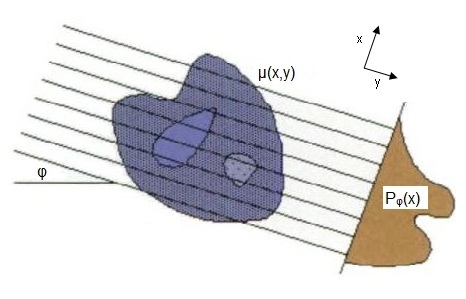
\includegraphics[scale=0.6]{intro_img/Russ_projection.jpg}
		\caption{Parallel ray geometry showing how a projection/view, $P_{\phi}(x)$, is recorded at angle $\phi$. The attenuation $\mu(x,y)$ within the sample is not uniform and projections must be taken from many angles to reconstruct a map of $\mu(x,y)$.  Here $x$ represents lateral position  and $y$ represents  depth. Figure adapted from \cite{russ2002image}.}
		\label{fig:projection}
	\end{figure}
	
	
	
	
	\begin{figure}[H]
		\centering
		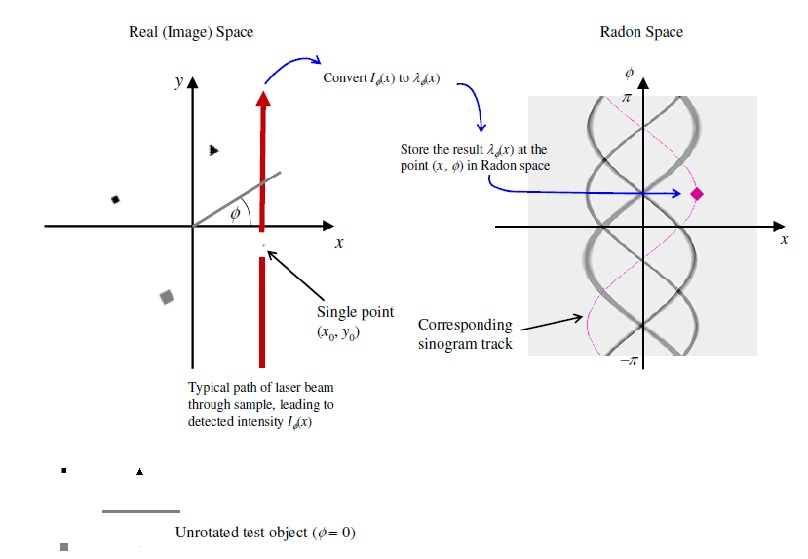
\includegraphics[width=\textwidth]{intro_img/Doran_2008_sinogram.jpg}
		\caption{Transformation from image space to Radon space demonstrated. Projection information is stored in Radon space. A 2-D image of Radon space is often called a sinogram. Different shapes produce characteristic tracks on the sinogram according to their symmetry upon rotation. Figure adapted from \cite{Doran:2008kh}.}
		\label{fig:sinogram}
	\end{figure}
	
	
	
	
	
	
	
	\subsection{Filtered Back-projection}
	\label{subsec:FBP}
	
	The information stored in a sinogram is used to reconstruct a map of attenuation within the sample. This is done through the process of back-projection.
	
	Simple back-projection involves  taking each projection point $P_{\phi}(x)$ and working back along the line integral, $L$, which created that projection in real space. Each point along $L$ is  attributed with the value $P_{\phi}(x)$. After doing this for all projection points, certain areas in real space are shaded darker as projections from different angles cross over. This builds up a picture of the shapes inside the sample. 
	
	Mathematically, back-projection can be described in terms of Fourier transforms (FTs). The 1-D FT of projection data for  angle, $\phi$, is given by
	\begin{equation}
	S_{\phi}(k_x) = \int P_{\phi}(x)\mathrm{e}^{-i x k_x}\, \mathrm{d}x
	\end{equation}
	where the FT maps $P_{\phi}(x)$ from the spatial domain to $S_{\phi}(k_x)$ in the frequency domain, also known as k-space.
	
	For the case of $\phi = 0$ this can  be written as
	\begin{align}
	S_{0}(k_x) &= \iint \mu(x,y) \mathrm{e}^{-i x k_x }\, \mathrm{d}x\mathrm{d}y \label{eq:1}\\
	&= \iint \mu(x,y) \mathrm{e}^{-i(k_xx +k_yy)}\, \mathrm{d}x\mathrm{d}y \label{eq:ky} \\ 
	&= \tilde{\mu}(k_x,k_y=0) \label{eq:3}
	\end{align}
	where $\tilde{\mu}(k_x,k_y)$ is the 2-D FT of $\mu(x,y)$.
	The extra term in (\ref{eq:ky}) is added  under the assumption that $k_y = 0$ giving $\mathrm{e}^{k_yy}=\mathrm{e}^{0}=1$. 
	
	Since the co-ordinate system can be chosen arbitrarily, equations (\ref{eq:1}-\ref{eq:3}) can be generalised for any angle $\phi$.
	This  is formalised in the Fourier Slice Theorem which states that the 2-D FT of $\mu(x,y)$ along the line at $\phi$ in k space is the same as the 1-D FT of the projection, $P_{\phi}(x)$ \cite{Doran:2008kh}.
	
	However, simple back-projection is flawed. As all the projections cross in the middle of the image, an artefact of high attenuation builds up there and edges of features in the sample are blurred.  In order to reconstruct more accurate images a mathematical trick called Filtered Back-projection (FBP) is used. 
	
	The blurring is similar to that of an out-of-focus system with point spread function (PSF) proportional to $\nicefrac{1}{f}$ where $f$ is the frequency \cite{russ2002image}. Therefore, to remove this blurring effect the image should be multiplied by the inverse of the blurring function in frequency space.
	
	The formula for reconstructing $\mu(x,y)$ using FBP involves a 2-D inverse FT of $S_{\phi}(k)$
	\begin{equation}
	\mu(x,y) = \frac{1}{2\pi} \iint \tilde{\mu}(k_x,k_y) \mathrm{e}^{i\left(k_xx+k_yy\right)}\, \mathrm{d}k_x\mathrm{d}k_y
	\end{equation}
	Converting to polar coordinates where $k_x=k\cos\phi$ and $k_y=k\sin\phi$ gives
	\begin{align}
	\mu(x,y) &= \frac{1}{2\pi} \int\limits_0^{2\pi} \int\limits_0^{\infty} \tilde{\mu}(k,\phi) \mathrm{e}^{ik\left(x\cos\phi+y\sin\phi\right)}k\, \mathrm{d}k\mathrm{d}\phi \\
	&= \frac{1}{2\pi} \int\limits_0^{2\pi}\left[\int\limits_0^{\infty}S_{\phi}(k)\mathrm{e}^{ikx'}k\, \mathrm{d}k \right]\, \mathrm{d}\phi \\
	&= \frac{1}{2\pi} \int\limits_0^{2\pi}Q_{\phi}(x')\, \mathrm{d}\phi
	\end{align}
	where $Q_{\phi}(x')$ is the projection filtered by in the frequency domain by multiplication with $k$. This is known as the ideal inverse filter, giving high weighting to high frequency components but low weighting to low frequencies. Other commonly used filters include the Hann,  Hamming, Butterworth, Shepp-Logan and Ram-Lak. Choice of filter can affect the quality of reconstructions \cite{russ2002image}.
	
	In order to use  FBP to reconstruct projections from OptCT two requirements of the Fourier Slice theorem must be satisfied. The first is that projections should be the result of rays travelling parallel to the optical axis through the sample. The second is that all points along a projection should contribute with the same weighting to the signal \cite{Wang:2007}. OptCT design considerations focus on satisfying these requirements to obtain high quality images.
	
	
	
	%Computational methods for improving reconstructions in OPT by Birk in 2011 \cite{Birk:2011}
	
	
	
	\subsection{Optics}
	
	The quality of reconstructed images is primarily limited by the quality of projection data. There are many aspects of FBP which can degrade image quality, such as the choice of filter and the number of projection angles acquired. However, there is also a fundamental limit on resolution achievable due to the optics of the system. Unlike x-ray CT, many OptCT systems use focusing optics to acquire projections. The type of optics used in OptCT has developed over the years, different set-ups are discussed in Sections~\ref{sec:dos} and~\ref{sec:tissue}. 
	
	The Rayleigh criterion states that two objects are just resolved when the centre of one Airy disk falls on the first minimum of the other object's pattern \cite{hecht2002optics}.
	Lateral resolution is given by this distance,
	\begin{equation}
	\Delta x=r_{Airy} = \dfrac{0.61n\lambda}{\rm{NA}}
	\label{eq:res}
	\end{equation}
	where $r_{Airy}$ is the radius of the Airy function. $n$ is the refractive index of the medium around the lens, $\lambda$ is the wavelength of light and NA$=n\sin \theta_{max}$ is the numerical aperture of the lens where $\theta_{max}$ is the acceptance angle of the optics.
	
	The depth of field (DOF) is the depth within the sample over which the image is acceptably sharp while the detector is kept in a constant position . At high NA the DOF is determined by wave optics while at low NA it is dominated by the geometrical `circle of confusion' \cite{shinya1997video}. Overall, the DOF can be expressed as a sum of these two effects
	\begin{equation}
	DOF = n_{bath}\left(\dfrac{n\lambda}{\rm{NA}^{2}} + \dfrac{n}{M\rm{NA}}e\right)
	\end{equation}
	where e is the pixel size of the CCD, $n_{bath}$ is the refractive index of the medium surrounding the specimen and $M$ is the lateral magnification.
	
	According to Nyquist, the Airy disc must be sampled more than twice per DOF distance to avoid aliasing \cite{Walls:2007jl}. This constrains the detector spacing to
	\begin{equation}
	e \leq M \dfrac{r_{Airy}}{2}
	\end{equation}
	so the maximum possible DOF is given by
	\begin{equation}
	DOF_{max} = n_{bath}\left(\dfrac{1.305\lambda}{\mathrm{NA}^{2}}\right)
	\label{eq:DOFmax}
	\end{equation}
	
	Comparing equations~(\ref{eq:res}) and (\ref{eq:DOFmax}) it can be seen that the choice of NA is very important.  Choosing a large NA will give high resolution however, the DOF will be limited. The NA has a more significant effect on DOF, having an inverse square relationship. To satisfy the second requirement of the Fourier Slice theorem, projection data should only be collected from regions within the DOF. If other regions are sampled they will have less weighting being less sharply focused. 
	
	Choosing the optimum NA will depend on the sample being imaged and as a rule, high resolution imaging is limited to small samples. Some methods to overcome this DOF barrier have been proposed by different groups and include, scanning the DOF through the sample \cite{Fauver:2005} and positioning the focal plane so only half of the sample is within  the DOF at one time and then taking $360^{\circ}$ worth of projections \cite{Sharpe:2002jp}. The advantages and disadvantages of these systems are discussed further in Section~\ref{subsec:OPT}.
	
	
	
	%\subsection{Common artefacts}
	
	%Axis of rotation problems. Corrections suggested by many groups. Recently by Dong in 2012 \cite{Dong:2012}  discuss method.
	
	%Walls 2005 \textit{Noise is Poisson distributed below 2\% on an averaged signal. Therefore artefactual effects must be kept below 1\%}
	
	%Ring artefacts are generated when a feature not associated with the dosimeter sample is present in the same place in all projections. A typical cause might be a bubble or scratch on the wall of the tank containing the matching liquid. (Directly from Doran 2008)
	
	%\newpage
	\section{Dosimetry}
	\label{sec:dos}
	\subsection{Laser scanning configuration}
	
	One of the first reported optical computed tomography (OptCT) systems was developed in the area of gel dosimetry. Accurate 3-D measurement of dose delivery in radiotherapy is extremely important in developing safe treatment plans. Specialist polymer gels, such as BANG\textsuperscript{\textregistered} \cite{Maryanski:1996}, respond to irradiation with changes in optical attenuation and scattering properties.  This makes them ideal for measuring 3-D dose distributions. Previously the irradiated gels were measured by MRI and x-ray CT. However, these are expensive imaging modalities. In 1996, Gore and Maryanski published the first system for scanning polymer gels using optical computed tomography \cite{Gore:1999tg}. In later comparisons, OptCT has been found to be more precise, have reduced noise and smoother line profiles than MRI for gel dosimetry \cite{Oldham:2001gs}, although these results have since been disputed. 
	
	Gore's system consisted of a  He-Ne laser source and large area photo-diode detector (see Figure~\ref{fig:gore_setup}). Translate-rotate acquisition was employed whereby the sample was rotated and projection data  acquired  by the photo-diode over $360^{\circ}$. Small angular steps between projections are necessary for high quality reconstruction \cite{russ2002image}. For a 2-D reconstruction, projections are acquired across a slice of the sample by translating the laser beam with mirrors. For 3-D information, the sample height  had to be manually adjusted and many 2-D slices acquired. This meant scanning an entire sample took  hours and lengthy scanning times are the chief disadvantage of the laser scanning method.  Accuracy of 5\% is reported and spatial resolution of 2mm, which is roughly the same as the laser beam width \cite{Gore:1999tg}.
	
	The idea of OptCT scanning in dosimetry was quickly developed by other groups. Laser scanning set-ups were published in 1996 by Tarte \textit{et al.},  \cite{Tarte:2006} and Kelly \textit{et al.}  \cite{Kelly:1998}.
	%\textit{Can't find the paper 1996 Kelly references in 1998 Med Phys says it doesn't exist.}
	Kelly \textit{et al.} claim to have independently developed their scanner which is very similar to that of Gore's. In in both Kelly's and Tarte's  scanners, the sample is rotated and translated using a stage whereas Gore used mirrors to translate the laser spot across the sample. 
	
	
	A commercial laser scanning OptCT system, OCTOPUS\texttrademark by MGS Research, Inc.
	(Madison, CT),  is an extension of Gore's original set-up with the addition of a platform capable of vertical movement for automated slice-selection \cite{Islam:2003gs}. For a number of years it was the only commercially available system and has been characterised by several groups \cite{Xu:2003cc, Islam:2003gs, Xu:2004iv, Sakhalkar:2009hb}. According to Oldham, characterisation of OptCT systems should include checks on geometric distortion, accuracy of reconstruction, scatter artefacts and reflection and refraction artefacts \cite{Oldham:2004cj}.
	
	
	
	
	%Upgraded laser Oldham 2004b \cite{Oldham:2004bv} - field photodiode mounted on a scanning arm to maintain constant distance between laser and detector. Check Oldham 2006 \cite{Oldham:2007eu}
	
	\begin{figure}[H]
		\centering
		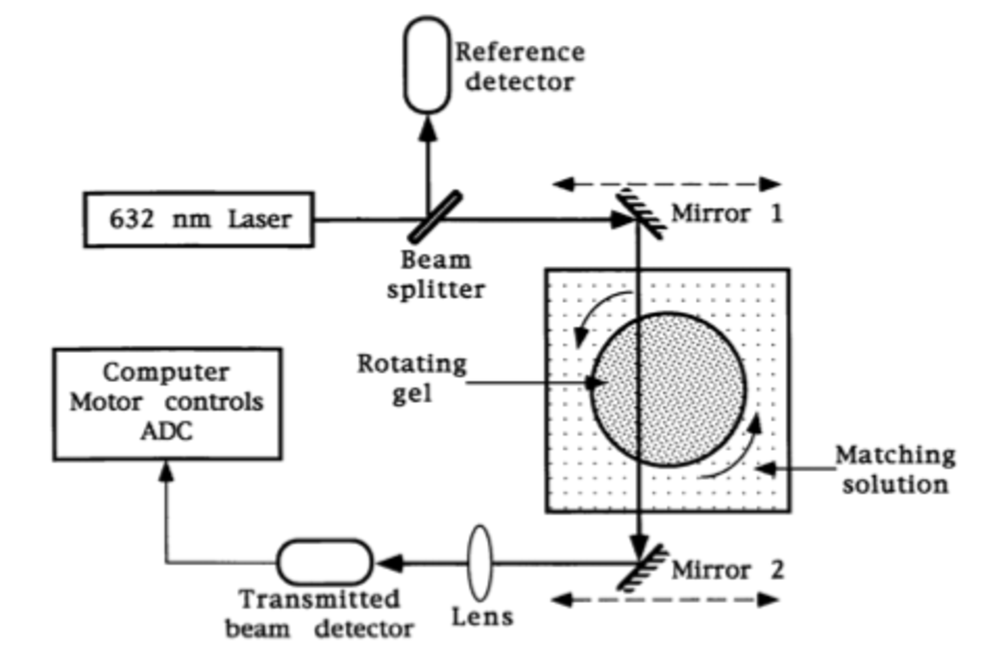
\includegraphics[scale=0.6]{intro_img/Gore_setup.pdf}
		\caption{A first generation,  Laser Scanning OptCT system developed by Gore. The sample is rotated and projections recorded at a number of angles. The  mirrors scan the laser beam across the sample but movement in the vertical direction is by manual adjustment only Figure adapted from \cite{Gore:1999tg}. }
		\label{fig:gore_setup}
	\end{figure}
	
	
	Laser scanning systems include a  beam splitter before the sample to create a reference beam. Dividing projections by the reference intensity  corrects for laser beam intensity fluctuations \cite{Gore:1999tg}.
	
	Refraction and reflection at container walls are significant concerns for all configurations of  OptCT. Generally, laser beams are incident on the gel container at a small angle, such as $5^{\circ}$, to avoid large reflection at the interface. The gel container is usually placed in a tank containing `matching fluid' with a refractive index close to that of the gel. This prevents significant refraction as the light passes into the gel. Doran found through ray tracing simulations that the refractive index of the walls of the matching tank and  gel container are not important compared to the gel and matching fluid. The optimum difference in refractive index between these two was interestingly found to be non-zero \cite{Doran:2001ee}. 
	
	To maximise the dynamic range of the system, coloured dye is commonly added to the matching fluid so the optical density of the matching fluid and gel are very similar \cite{Krstajic:2006kna}. 
	
	
	
	
	\subsection{Pixelated detector based systems}
	
	The first CCD based OptCT system was developed in a separate field in 1996, investigating self-organising chemical structures \cite{Winfree:1996}.
	In 1997 it was adopted for dosimetry by Tarte \textit{et al.} who employed an incoherent white light source and CCD camera detection \cite{Tarte:2007}. The advantage  of a pixelated detector based system  is that an entire 2-D projection can be imaged at once, potentially increasing the scanning speed by several  orders of magnitude depending on the data through-put rate. Tarte's system used a divergent light source and diffusing screen to measure optical density in a thin gel section (see Figure~\ref{fig:tarte_ccd_setup}). 
	%For a very thin sample this adequate however, more sophisticated optics are required for bigger samples. \textbf{Does tarte reconstruct at all?}
	
	\begin{figure}[H]
		\centering
		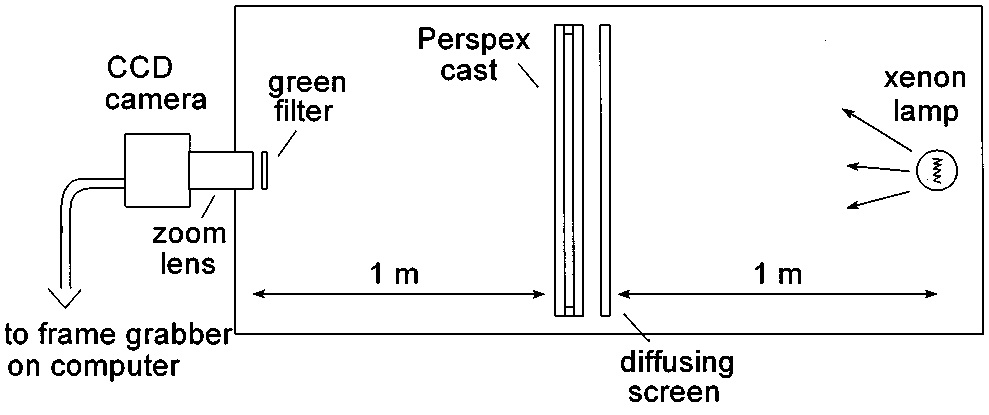
\includegraphics[scale=0.4]{intro_img/Tarte_1997_ccdsetup.jpg}
		\caption{Diagram of the first CCD-based  OptCT system for dosimetry, developed by Tarte \textit{et al.} It uses  divergent illumination from a white light source and CCD camera detection to record an entire 2D projection at once.   Figure adapted from \cite{Tarte:2007}. }
		\label{fig:tarte_ccd_setup}
	\end{figure}
	
	
	The accuracy of Tarte's system  was checked by comparison with the standard measure of dosimetry, the parallel plate ionisation chamber. It was found to be on average within 3\% of the value from the ionisation chamber \cite{Tarte:2007}. A comparison between Tarte's laser scanning and CCD set-ups found that they had similar spatial resolutions. The CCD method had improved speed of acquistion but suffered from consistently worse SNR as a photodiode detector can collect many more photons per `pixel' than a CCD camera \cite{Tarte:2007}.
	
	%The laser system 'pixel' is defined by the region illuminated by the laser spot while the photodiode has a much larger area than the spot, so it collects even photons which have diverged from a straight line. 
	
	Advances in technology have meant that  high quality detectors are much more affordable. A cheaper alternative to very high quality CCD cameras is the CMOS (Complementary Metal-Oxide-Semiconductor) detector which has the potential for higher resolution and dynamic range \cite{Doran:2008kh}. Using a higher quality detector would improve many OptCT systems  in terms of scanning speed and reduced artefacts \cite{Tarte:2007, Doran:2001ee}.
	
	
	\paragraph{Parallel beam configuration:} One method to reconstruct 3-D images with a CCD or CMOS detector is to create a broad parallel beam. This allows the use of parallel reconstruction algorithms, very similar to those used for x-ray CT. Each 2-D projection image recorded corresponds to one row for every slice in the 3-D reconstruction sinogram \cite{Doran:2008kh}.
	Telecentric optics, in which the chief rays are parallel to the optical axis, are key in the design of this configuration \cite{Walls:2005ja}. Telecentric optics can be achieved either through a careful arrangement  of  a large converging lens before the sample and standard camera lens  \cite{Doran:2001ee} (see Figure~\ref{fig:doran_ccd_setup}) or through an expensive telecentric lens \cite{Sakhalkar:2008exa}. The process of forming a parallel beam results in non-uniformities in the lightfield. This is compensated for by dividing by a `correction' or `open lightfield', image which is a projection taken with no sample in the tank \cite{Doran:2001ee}.
	
	Telecentric lenses give the advantages of parallel rays and almost constant magnification throughout the sample \cite{Oldham:2007ku}. This helps to satisfy the requirements of the Fourier Slice Theorem for high quality reconstruction mentioned in Section~\ref{subsec:FBP}.
	
	
	\begin{figure}[H]
		\centering
		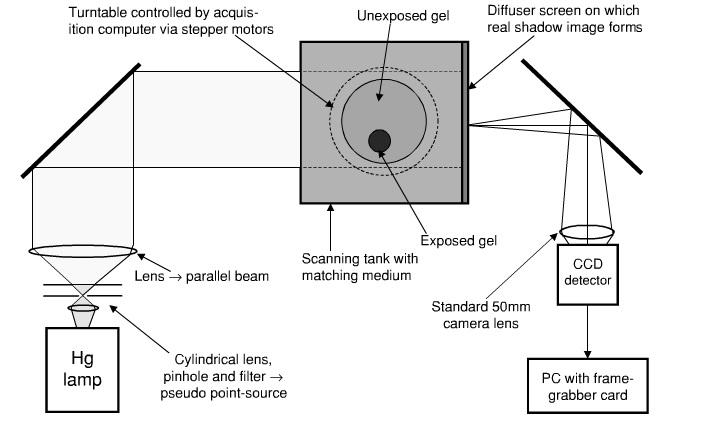
\includegraphics[scale=0.55]{intro_img/Doran_2001_ccdsetup.jpg}
		\caption{Diagram of a parallel beam  OptCT system, developed by Doran \textit{et al.} Telecentric optics create a parallel beam.  Figure adapted from \cite{Doran:2001ee}. }
		\label{fig:doran_ccd_setup}
	\end{figure}
	
	
	
	Initial systems  suffered from `graininess' due to the unstable gain of cheap CCD cameras and granularity of the diffusing screen \cite{Doran:2001ee}. Superior optics meant later systems did not require a diffuser and instead lenses were used to image directly onto the CCD \cite{Krstajic:2006kna}.  
	
	%Doran \textit{et al.} proposed some methods of correcting these problems. Oscillating the diffuser screen at high frequency ``\,`smears' out the granularity'' while randomly horizontally displacing the CCD camera by a few pixels  between acquisitions can reduce the effect of `bad'  pixels \cite{Doran:2001ee}.
	% The parallel configuration appears to be more susceptible to schlieren artefacts caused by refractive index inhomogeneities in the sample \cite{Krstajic:2007hk}.
	
	
	
	
	
	
	\paragraph{Cone beam configuration:}
	Wolodzko \textit{et al.} published the first cone beam OptCT system with CCD detection for gel dosimetry \cite{Wolodzko:1999}. One advantage of this configuration is the optics for producing a cone beam are much simpler than those for producing accurate parallel beams \cite{Doran:2008kh}. However, the reconstruction is computationally more complex \cite{hsieh2003computed}. A commercial cone-beam system, Vista\texttrademark by Modus Medical Devices Inc. (London, ON, Canada),  is available and reviewed recently by Olding \textit{et al.} \cite{Olding:2011eta}.
	
	
	\begin{figure}[H]
		\centering
		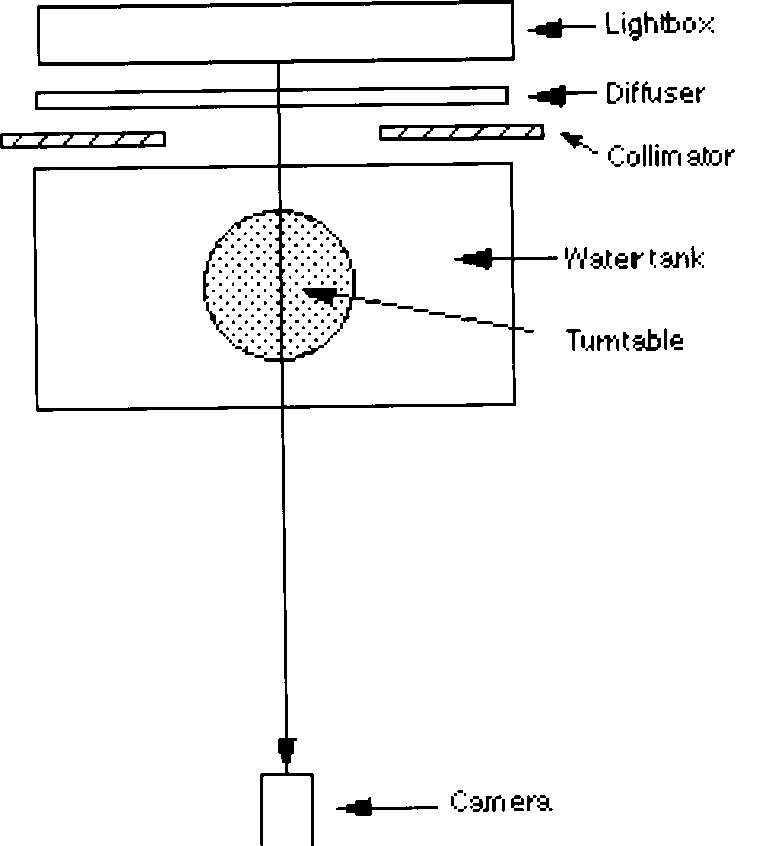
\includegraphics[scale=0.3]{intro_img/Wolodzko_1999_conesetup.jpg}
		\caption{The first cone-beam CCD configuration for OptCT. The optics are much simpler than for parallel beam systems. Figure adapted from \cite{Wolodzko:1999}.}
	\end{figure}
	
	
	There has not been experimental comparison of parallel and cone-beam systems. However,  Doran suggests that while cone-beam is usually somewhat cheaper due to simplified optics, modern parallel-beam systems have better scatter-rejection and may have fewer stray light problems \cite{Doran:2008kh, Olding:2011eta, Thomas:2011eja}.
	
	
	
	
	
	
	
	
	
	
	%Refraction and reflection at container walls are significant concerns for all configuration of dosimetry with OptCT. These problems have been investigated with Mie theory modelling of light paths. Doran found through ray tracing simulations that the refractive index of the walls of the matching tank and  gel container are not important compared to the gel and matching fluid. The optimum difference in refractive index between these two was calculated to be 0.0025 and not zero as originally thought.\cite{Doran:2001ee} Another counter intuitive finding was that the ideal gel container wall thickness is not the thinnest possible but some median thickness which 
	
	%Problems with vial walls misrepresentation due to refractive index mismatch. \cite{Doran:2001ee}
	
	%Illumination is chosen based on the configuration used and the wavelength range which is optimum for dose measurement.  
	%Stray light minimisation is very important in OptCT. Dark room, shield the illumination source. Interference filters. REF 
	
	
	%Repeatability of experiments, have locking method for samples. REF
	%Centre of rotation recovery, mostly post-processing. In theory section. 			
	
	%\textit{The first is laser based and has several design considerations including minimisation of interference effects and stray light; scatter from optical components and the radiochromic gels themselves, reflection; dynamic range; wavelength selection; wall corrections plasma discharge from lasers; temperature changes; and the characterisation of detectors.A general disadvantage of scanners based on pixelated detectors together with a wide beam is the possible introduction of artefacts by refractive index inhomogeneities (schlieren). } from \cite{Doran:2008kh}
	
	
	
	
	
	
	
	%\newpage
	\section{Tissue imaging}
	\label{sec:tissue}
	\subsection{Optical Projection Tomography}
	\label{subsec:OPT}
	Another version of OptCT was  developed by Sharpe \textit{et al.} in the area of 3-D microscopy for gene expression studies \cite{Sharpe:2002jp}. Although this set-up in 2002 came after Gore's they are apparently independent and Sharpe named his technique Optical Projection Tomography (OPT).
	
	Although other techniques for 3-D microscopy are well established, OPT offers some unique advantages. 
	Confocal microscopy offers high resolution images up to a depth of about 1mm \cite{Webb:1996}. However, it is limited to fluorescent signals meaning many optical stains used routinely in histology would not work. Optical coherence tomography (OCT), which is commonly used in ophthalmology, is capable of micrometer-scale resolution but with  depth limited to 2-3mm in tissue \cite{huang1993optical}. Both of these techniques generate tomographic images through sectioning whereas OPT is a projection based tomography technique \cite{Sharpe:2003cm}. Avoiding sectioning is important in producing truly representative 3-D images \cite{Oldham:2007ku}. Another advantage of  OPT is its ability to  image much larger specimen, with depth of around 3cm being reported \cite{Oldham:2007ku}. This superior imaging depth not just due to clarification of the samples, discussed in Section~\ref{sec:clearing}. OCT and confocal systems have also been tested with clearing agents and the reported gains in depth vary between 20-150\% in OCT \cite{Tuchin:2002} which is significantly shallower than OptCT.
	
	
	Sharpe's original system uses a microscope to focus projections of a mouse embryo onto a camera imaging chip.  Sharpe reports some impressive images as reproduced in Figure~\ref{fig:SharpeOPT}. Use of the microscope gives resolution of about 5-10$\mu$m meaning single-cell membranes, around 10$\mu$m thick, can be seen\cite{Sharpe:2002jp}. However, the high NA  optics which give high resolution limit the DOF. Sharpe decided to circumvent the problem of a low DOF by positioning the rotational axis so only half the specimen was in focus at once. $360^{\circ}$ of projections were taken to collect in-focus data from all points. The problem with only having half of specimen in focus at once is that unfocused light is superimposed upon the focused data and included in the reconstruction. This leads to blurring, which is worse with distance from the axis of rotation. Walls \textit{et al.} proposed a method of correcting this defocusing effect using a frequency-distance filter, as described by Xia for SPECT \cite{xia1995fourier,Walls:2007jl}. The filter narrows the PSF to in-focus data allowing in-focus, high resolution images to be reconstructed \cite{Walls:2007jl}.
	
	
	
	In dosimetry the refractive index within the polymer gels is roughly uniform. In tissue this is not the case, with scattering and refraction occurring at cell membrane interfaces. To make high resolution reconstruction through back projection possible, light paths through the specimen must be able to  be approximated as parallel line integrals meaning refraction must be minimised. A process called optical clearing or clarification is employed which renders tissue optically transparent. An optical clearing agent (OCA) replaces the lower refractive index intra-cellular fluid. It acts as a matching fluid within the sample itself. The mechanism for this differs between agents, see Section~\ref{sec:clearing} for more detail. 
	
	
	
	
	
	\begin{figure}[H]
		\centering
		\subfigure[OPT setup]{\label{subfig:OPTsetup}
			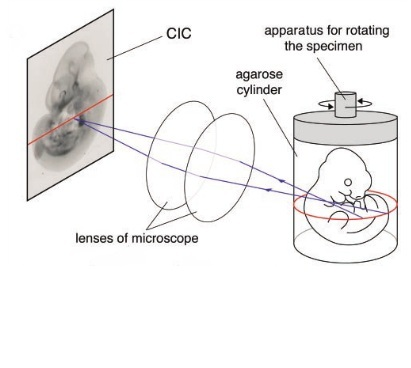
\includegraphics[width=0.5\textwidth]{intro_img/Sharpe_2002_setup.jpg}}
		\subfigure[Mouse images]{\label{subfig:OPTmouse}
			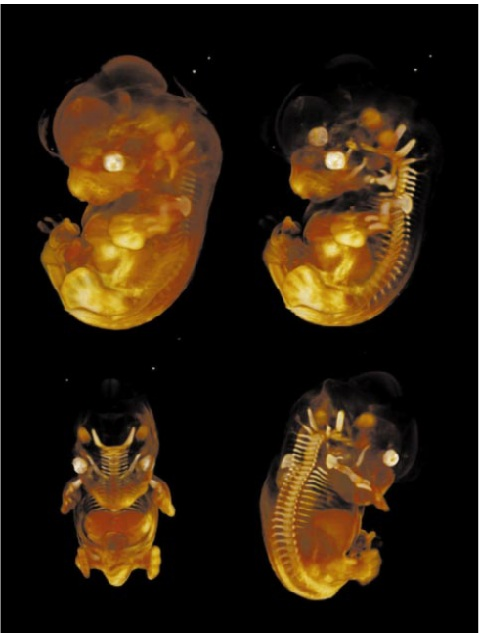
\includegraphics[scale=0.5]{intro_img/Sharpe_2003_mouse.jpg}}
		\caption{Part (a) shows the optical set-up for the first OPT system by Sharpe. CIC indicates the camera imaging chip. A microscope is used to focus projection images onto the CIC. The specimen is set in agarose gel for stability. Figure adapted from \cite{Sharpe:2002jp}. Part (b) shows some false colour images of a TS21 mouse embryo stained with alcian blue and imaged with OPT. The images have varying degrees of opacity allowing control of which internal organs are seen. Figure  adapted from \cite{Sharpe:2003cm}.}
		\label{fig:SharpeOPT}
	\end{figure}
	
	
	
	
	In 2005 Fauver reported a modified version of OPT capable of imaging single cell nuclei with 0.9$\mu$m resolution (see Figure~\ref{fig:fauver_setup})\cite{Fauver:2005}. The OPT microscope includes a rotation stage and  piezoelectrically driven objective lens. In a technique similar to Hausler \cite{hausler1972method} the objective lens is scanned axially to create an extended DOF image which is also known as a pseudo-projection. The extended DOF means features have the same focus from all angles, allowing high resolution reconstruction. However, this is not a truly quantitative technique, hence pseudo and not true projections are recorded. A high NA lens gives high resolution at the expense of low depth of field. If such high resolution is not required, lower NA optics would be a more quantitative way to generate  projections than scanning a high NA lens.
	
	
	
	\begin{figure}[H]
		\centering
		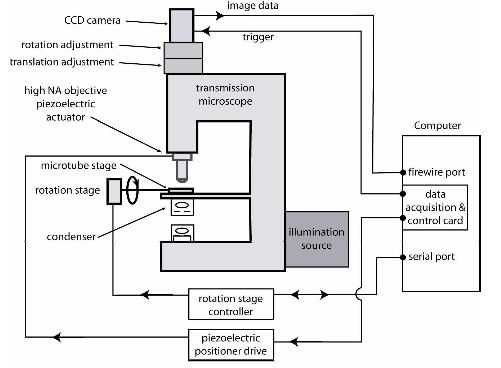
\includegraphics[scale=0.8]{intro_img/Fauver_2005_setup.jpg}
		\caption{OPT microscope for imaging single cell nuclei. A microcapillary tube injected with cells is rotated with sub-micron precision. The piezoelectric objective lens is scanned axially to create extended depth of field images. Figure adapted from \cite{Fauver:2005}.}
		\label{fig:fauver_setup}
	\end{figure}
	
	
	Wang and Wang have reported an improvement to OPT giving higher axial and lateral resolution, even for slices far from the optical axis \cite{Wang:2006hy, Wang:2007}. As previously mentioned, to obtain high quality reconstructions the projections should closely approximate a line integral of parallel rays passing through the sample \cite{Wang:2006hy}. This is not exactly the case for  OPT, which limits the best resolution possible. Wang proposed placing an iris at the back focus of the objective lens. This reduces divergence of the projection rays from paths parallel to the optical axis giving qualitatively better resolution.
	
	
	\subsection{Fluorescent/emission  OptCT}
	\label{subsec:eOPT}
	
	Sharpe was the first to identify the possibility of using OPT to image fluorescent stains in biological specimen \cite{Sharpe:2002jp}. There are a wide range of fluorescent optical stains in use in histology making this development particularly useful for biological imaging. It also offers the advantage of being able to record multiple signals independently unlike  transmission OPT (tOPT) \cite{Sharpe:2002jp}. 
	
	%Include a paragraph on terminology? OPT and OptCT seem to be able to be used almost interchangeably in later tissue imaging papers. Need to pick one name and explain other groups use other terminology.
	
	Optical emission CT (OptECT) also known as emission OPT (eOPT) is the optical equivalent of SPECT (single photon emission computed tomography) \cite{Oldham:2007ku}.  Instead of measuring the attenuation of photons through a sample (like tOPT), eOPT signal comprises of fluorescence photons emitted along a ray path \cite{Walls:2005ja}.
	
	
	
	Some changes from the set-up (see Figure~\ref{fig:eOPTsetup}) from tOPT  include the addition of a narrow bandwidth excitation filter before the sample. This selects for the excitation wavelength of the fluorescent marker being used in the sample. The illumination is perpendicular to the detector to avoid detection of the illumination light rather than fluorescence. An emission filter before detector selects for the longer emission wavelength of the fluorophores, again to avoid contamination from auto-fluorescent and ambient photons being picked up by the CCD. To avoid photobleaching systems often include a shutter to turn off the lamp when not imaging.  The image forming optics is the same as for tOPT, although the reconstruction and artefacts are different \cite{Walls:2005ja}.
	
	
	
	Oldham \textit{et al.} have adapted Sharpe's eOPT set-up by changing from microscope to bench-top apparatus, similar to their dosimetry OptCT system \cite{Oldham:2006, Oldham:2007ku}. Microscope based systems suffer from poor DOF as the optics are designed to image flat samples.  Oldham's custom made set-up employs telecentric optics giving much improved DOF capable of imaging samples up to 3cm \cite{Oldham:2007ku}. However, better DOF is achieved at the cost of worse lateral spatial resolution and this trade-off must be considered with respect to the information required from the specimen \cite{Krstajic:2006kna}.   A comparison of microscope and telecentric systems would be very interesting in future work.
	
	
	
	\begin{figure}[H]
		\centering
		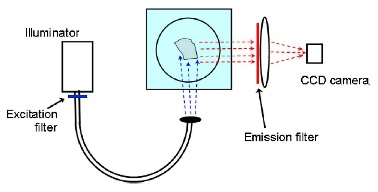
\includegraphics[scale=1]{intro_img/Oldham_2007ku_eCTsetup.jpg}
		\caption{Example of setup for OptECT/eOPT imaging. Filters are used to select for the excitation and emission wavelengths of the fluorescent stain. This set-up can give an image but no quantitative information without specialised reconstruction techniques discussed below. Figure adapted from \cite{Oldham:2007ku}.}
		\label{fig:eOPTsetup}
	\end{figure}
	
	
	
	
	
	
	
	%\subparagraph{Quantitative eOPT:} 
	There are several reasons why eOPT data is not quantitative. The most significant problem is that an unknown number of emitted photons are attenuated within the sample. This requires a mathematical model of attenuation for correction. The second problem is that some incident photons are attenuated before they can cause excitation.  This can be compensated for with simultaneous illumination from multiple angles \cite{Kim:2008eua}.  Another problem identified by Darrell \textit{et al.} is a defocusing effect caused by the lower intensity of of fluorophores positioned outside of the focal plane. Darrell's method of quantifying eOPT data involved a Fourier optics based model which accounted for the defocusing effect and isotropic emission attenuation \cite{Darrell:2008gd}. A weighting function was calculated based on this model. The function was used in FBP and acts as a window function, spreading the projection information unevenly over the reconstruction image plane.
	
	Kim \textit{et al.} have also published a method for correction of emission attenuation \cite{Kim:2008eua}. This method is similar to those used for attenuation correction in SPECT. A co-registered image from tOPT is used to construct an attenuation map and calculate attenuation-survival probabilities for the sample. The probabilities are then used in an iterative OSEM (ordered-subsets expectation-maximisation) reconstruction \cite{Kim:2008eua, hudson1994accelerated}. This attenuation correction method was tested using a  phantom with known fluorescent fibres and corrected images showed more uniform intensity across the three fibres, differing by 4\% in the corrected images but as much as 24\% in uncorrected data \cite{Kim:2008eua}.
	
	In an extension of Kim's method, Thomas \textit{et al.} were the first to report a comprehensive correction for  eOPT \cite{Thomas:2010gt}. Their iterative method corrects for both emission and excitation attenuation and non-uniformities in the light source. 
	Tests of their technique using phantoms show that it can give quantitative information of 3-D fluorophore concentration. This is could be very biologically useful, for example looking at uptake of drugs in tumour treatment. 
	
	
	
	
	
	
	%\subparagraph{Live eOPT:} 
	There have been attempts at performing OPT  on live specimen \cite{Boot:2008dt, Vinegoni:2008ix, Colas:2009}. The chief difficulties in this are developing a method limiting scatter and refraction  whilst also keeping the specimen alive. Boot and Sharpe reported their efforts for \textit{in vitro} time-lapse quantitative eOPT  imaging through tracking GFP expression of a growing mouse embryo limb bud, about 1mm in size \cite{Boot:2008dt}. 
	Live OPT has also been used in molecular imaging tracking a changing 3-D gene expression pattern \cite{Colas:2009}.
	Vinegoni \textit{et al.} reported \textit{in vivo} imaging of Drosophila melanogaster pupae without clearing or matching fluids \cite{Vinegoni:2008ix}.  As there is no clearing involved and a mathematical model is required for reconstruction Vinegoni called this `mesoscopic' imaging rather than OPT/OptCT.  
	%A polarisation analyser in front of the CCD rejects highly scattered photons which lose their polarisation state. 
	Although gathering some biologically interesting information, the resolution was much worse than conventional OPT limiting the applications for this technique. It would be fantastic to be able to monitor tumour development in 3-D. Doing live imaging means the mouse could be its own control, instead of sacrificing many mice at different stages of tumour development. This may not be possible due to limited size and resolution.
	
	
	
	
	%Walls: Have to be careful with eOPT systems using mercury arc lamp as it suffers from fluctuations which get worse with age, as bad as 10\%. This can introduce a smearing artefact due to the high-frequency component of the fluctuations. Walls ran simulations to calculate the best way to compensate for the fluctuations using intensity measurements from the lamp itself and a Gaussian distribution for noise with sd of 1.2\% and 5\% for an older lamp. Computational method explained on page 7. Relevant?
	
	
	
	
	
	
	%\newpage
	\section{Optical Clearing}
	\label{sec:clearing}
	
	%Need for refractive index matching to ensure parallel beam assumption is true enough that we can emloy traditional reconstruction techniques. 
	Optical clearing or clarification is a very important step in OptCT imaging of tissue. Tissue is made up of many components of different refractive indices, meaning there are many optical boundaries for scatter and refraction to occur at. This is the reason why visible wavelength light does not penetrate very far in tissue. To use the parallel ray assumption  in CT reconstruction, refraction and scatter at cell membrane interfaces within the sample must be minimised \cite{Oldham:2006}.  This is accomplished with clearing.
	
	During clearing, intracellular  fluid is replaced with a optical clearing agent (OCA). There are many choices of OCA but they should all have refractive indices matching the tissue to be imaged and be hyperosmolar (i.e. have a very high solute concentration) \cite{tuchin2007tissue}.
	
	
	A very popular technique for clearing is the Optical Immersion technique. The sample is set in agarose gel for stability. The gel contains pores which allows diffusion of the OCA. The most commonly used OCAs for OPT are benzyl-alcohol-benzyl-benzoate (BABB, refractive index 1.55) or methyl salicylate (MetSal, refractive index 1.53). These are both aromatic organic solvents and are not miscible in water. Therefore a graded sequence of ethanol and OCA solutions is required to replace the intracellular water with the OCA \cite{Oldham:2006}. 
	
	Some OCAs, including glycerol and dimethyl sulfoxide (DMSO), can be directly applied to the tissue without need for graded ethanol solutions. However, they have been shown to be less effective than BABB and MetSal and cannot penetrate deeper than 1cm \cite{Oldham:2006}.  Glycerol may be more suitable for \textit{in vivo} or live studies as it is biologically inert however DMSO would not be suitable due to high toxicity \cite{Wen:2009is}.
	
	%BABB has n=1.56 while water is n=1.33, what is n for tissue? \cite{Walls:2005ja}
	
	Glycerol appears to be the best OCA for clarification of the skin \cite{Vargas:1999, Wen:2009is}. Its refractive index (1.46) is very similar to that of collagen which is the main scatterer in skin. What is unique about glycerol is the clearing effect is reversible upon rehydration with phosphate buffered saline solution \cite{Vargas:1999}. 
	
	The mechanism for how OCAs bring about optical clarification is not clear. It was previously thought the effect was purely due to refractive index matching however some work has shown that clearing skin with alcohol doesn't correlate with the OCA's refractive index \cite{Choi:2005, Mao:2008}. Additionally, glycerol's reversibility indicates that its clarification mechanism is different to other agents. Some  proposed mechanisms include the dissociation of collagen (unravelling of the fibrous structure) and  dehydration (reducing the space between scatterers) as additional clearing effects \cite{Yeh:2003, Wen:2009is}.
	
	
	
	
	Preserving fluorescent signal is very important when clearing for eOPT/OptECT applications. Oldham and Sakhalkar have tested some clearing and fixing protocols with different fluorescent proteins \cite{Sakhalkar:2007hp, Oldham:2008dfa}. Although it is common to fix tissue samples with paraformaldehyde (PFA), it was found that this resulted in an almost complete loss of fluorescent signal. Fixation with ethanol was found to preserve fluorescence and keep fluorophores robust upon application of BABB or MetSal. Although BABB was found to give better optical clarity in general, MetSal gave better fluorescence preservation. The optimal procedure was a combination of ethanol fixation and MetSal clearing which was tested on red and green fluorescent proteins (RFP and GFP) \cite{Sakhalkar:2007hp}.
	
	
	The exact concentrations of OCA needed and the specific OCA used will depend on the tissue and form of imaging to be performed. Finding the optimum chemicals for our purpose will involve trial and error as it has been previously shown that clearing effects are unpredictable due to the complex nature of the interactions between OCA and tissue \cite{Wen:2009is}.
	
	
	
	%\newpage
	\section{Optical Staining}
	\subsection{Staining for Cancer Markers}
	
	The goal of our investigation will be characterising MRI contrast in tumours by comparison with detailed 3-D maps of histological stains given by OptCT. Staining for tumour recognition and characterisation is a well established area for histology and will be briefly reviewed here.  One aspect to be investigated is how these stains work in the presence of OCAs. Unfortunately, Oldham has not found a method of combining immunohistological stains with clearing procedures, making \textit{in vivo} staining the most attractive option at present \cite{Oldham:2008dfa}.
	
	
	
	%Being able to use optical stains is extremely useful for computer recognition of organs, can pick better thresholds. \cite{Sharpe:2003cm}
	
	%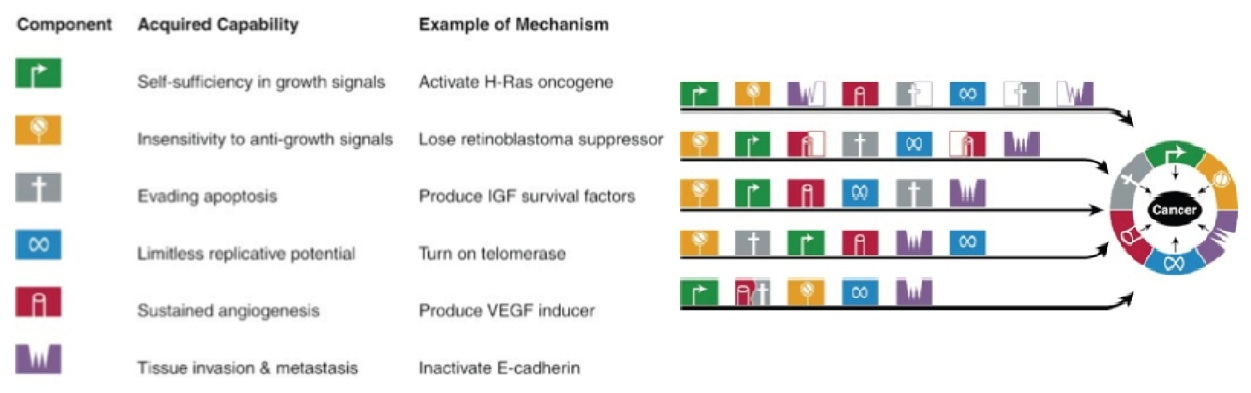
\includegraphics[scale=0.45]{Hanahan_2000_hallmarks.jpg}
	%\caption{Diagram showing the six hallmarks of cancer. These adaptations are believed to be necessary for  tumours to become macroscopic. The changes can be acquired in many different ways and in different orders chronologically, as illustrated in the diagram. Figure adapted from \cite{Hanahan:2000}}
	
	%\begin{figure}[H]
	%\centering
	%\subfigure[Traditional Hallmarks]{\label{subfig:hallmarks}
	%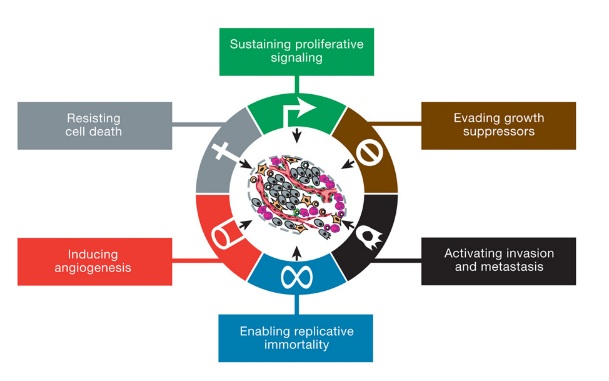
\includegraphics[width=0.45\textwidth]{Hanahan_2011_hallmarks.jpg}}
	%\subfigure[New hallmarks]{\label{subfig:newhallmarks}
	%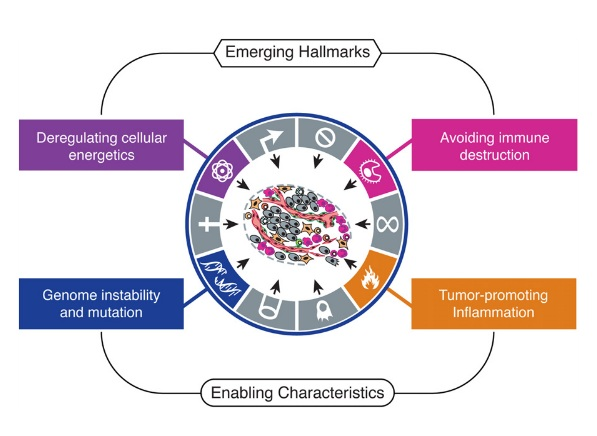
\includegraphics[width=0.45\textwidth]{Hanahan_2011_emerginghallmarks.jpg}}
	%\caption{Diagram showing the six hallmarks of cancer (\ref{subfig:hallmarks}) and some emerging characteristics that appear to also be necessary for tumours to become macroscopic (\ref{subfig:newhallmarks}). The changes can be acquired in many different ways and in different orders chronologically. Figure adapted from \cite{Hanahan:2011gua}}
	%\label{fig:hallmarks2011}
	%\end{figure}
	
	
	The primary hallmarks of cancer, which are believed to be present in virtually all tumours, are listed in Figure~\ref{fig:padhani} \cite{Hanahan:2000}. How these acquired capabilities are gained differs between individual tumours. However, there are some common pathways that can provide targets for therapy. The hallmarks also give some clues for imaging tumours (see Figure~\ref{fig:padhani}). Certain genes have been found to be very common in the route to gaining these capabilities. For example, inactivation of the p53 tumour suppressor gene is found in more than 50\% of  human tumours, giving the tumour cells the ability to evade apoptosis (programmed cell death). This gene can be tracked via reporter genes, such as HSV1-tk(GFP) which can then be imaged with positron emission tomography (PET) \cite{Doubrovin:2001}.  
	
	The area of molecular imaging is relatively new and usually involves the use of a reporter gene and complimentary reporter probe, the accumulation of which gives an indication of gene expression \cite{Blasberg:2003}. Different reporter probes can be imaged with MRI, PET, SPECT and optical techniques. Optical techniques have the advantage of being more cost and time-effective than MRI or nuclear methods. As mentioned before, OptCT has the additional advantage of better depth penetration than other common optical imaging methods such as confocal microscopy.
	
	%One such common target is the vascular endothelial growth factor (VEGF) which is often overexpressed in tumours and is important for angiogenesis. Blocking VEGF can stop additional blood flow to the tumour and restrict its growth. 
	
	%Other possible hallmarks have been identified which include evasion of anoikis (cell death signals caused by loss of cell-ECM contact) and increased glucose consumption through increased glycolysis. \cite{Gatenby:2008} 
	
	
	
	\begin{figure}[H]
		\centering
		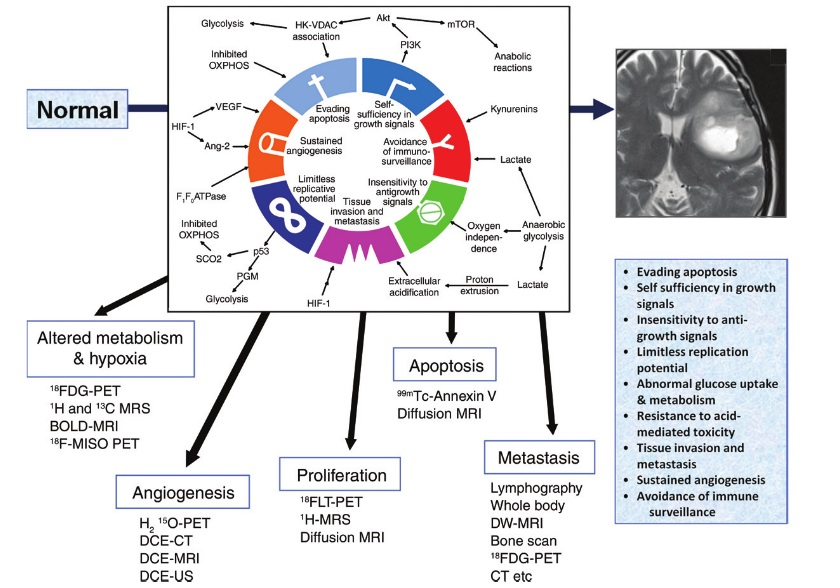
\includegraphics[scale=0.6]{intro_img/Padhani_2010_hallmarks.jpg}
		\caption{Diagram linking functional imaging modalities to the hallmarks of cancer. Figure adapted from \cite{Padhani:2010hfa}.} %\textit{DW}:diffusion weighted, \textit{DCE}:dynamic contrast agent, \textit{Bold}: blood oxygenation-level dependent,\textit{US}: Ultrasound, \textit{MRS}: magnetic resonance spectroscopy, \textit{Ang-2}: angiopoietin-2, \textit{FLT}: fluorothymidine, \textit{HK}: hexokinase, \textit{OXPHOS}: oxidative phosphorylation, \textit{PGM}: phosphoglycerate mutase, \textit{PI3K}: phosphatidylinositol 3-kinase, \textit{SCO2}: synthesis of cytochrome c oxidase 2, \textit{VDAC}: voltage-dependent anion channel. Figure adapted from \cite{Padhani:2010hfa}.}.
		\label{fig:padhani}
	\end{figure}
	
	
	Fluorescent proteins have revolutionised the area of tumour imaging, allowing real-time imaging of tumour angiogenesis, metastases, cell invasion and motility \cite{Hoffman:2005}. Using these proteins can give visualisation of a single metastatic  cell in normal tissue, far beyond the ability of histology which is the current gold standard of imaging \cite{Hoffman:2009}. The ability to colour-code cells according to genotype and phenotype is a massive advantage when monitoring the progression of tumours and their response to treatment.
	Some disadvantages of using fluorescent markers include the complication of  quantifying the data, high auto-fluorescence in the blue-green window which limits SNR, fluorophore photobleaching and high levels of scatter and attenuation of photons in tissue \cite{Gross:2005}. However, these problems are being solved as fluorescent imaging becomes more common-place. 
	
	
	The most common fluorescent marker used is  green fluorescent protein (GFP) and its spectrally shifted variants with emission ranges from 442-645nm \cite{Hoffman:2005}. The GFP gene was first cloned from \textit{Aequorea victoria} jellyfish and has since been humanised giving high expression and signal for use in mammals \cite{Hoffman:2009}. They are popular markers due to their high extinction coefficient and high quantum yield giving very bright and efficient fluorescence. The variants are spectrally different enough to can be used simultaneously, marking different aspects of the biology \cite{Hoffman:2005}. 
	
	With the discovery of red and NIR fluorophores, fluorescent optical molecular imaging is becoming  more widespread. These markers avoid the problem of blue-green autofluorescence that GFP experiences and also have slightly deeper penetration due to the therapeutic window in tissue. The first red fluorescent protein (RFP) was cloned from \textit{Discosoma} coral in the late 1990s and has been modified giving DsRed-2, a very bright protein with emission peak at 588nm. Other longer wavelength variants have been developed such as mPlum and mCherry however these are less bright \cite{Hoffman:2009}. A newer, very bright red marker called Katushka looks very promising with high photo-stability. Its excitation and emission wavelengths of 588nm and 635nm respectively are ideal for tissue being lowly absorbed by both tissue and haemoglobin \cite{Shcherbo:2007}.
	
	
	Other fluorescent stains which may be interesting include  Doxorubicin, which is a fluorescent drug  giving a measure of drug delivery \textit{in vivo} and Evan's blue, a permeability marker which is used clinically. 
	Some non-fluorescent stains which would be used for tOPT include Alcian blue which stains cartilage, and Pimonidazole which is a clinically used hypoxia marker giving quantitative and qualitative measures of hypoxia in tissue \cite{Varia:1998}. 
	
	%Resins such as Mercox and Microphil. HERC (Spelling?), which is a perfusion marker administered \textit{in vivo}
	
	
	One issue with choosing stains for use in OptCT is finding stains which can diffuse through a whole tumour. Stains administered \textit{in vivo}, such as by tail injection, may be preferable rather than trying to stain a large volume of tissue after dissection. For example, Soufan \textit{et al.} monitored gene expression during cardiac development in 2003. Their preferred stains  could not penetrate the entire embryo heart and they were forced to take slices, losing valuable 3-D information \cite{Soufan:2003cd}. 
	
	
	\subsection{Optical Staining in OptCT}
	
	One example of fluorescent proteins being used for OptCT imaging is by Kim \textit{et al.} in 2008 \cite{Kim:2008eua}. A tumour cell line was genetically labelled with GFP and RFP which were used to image hypoxia-indcible factor 1 (HIF1) and necrotic regions respectively. Tumour micro-vasculature was labelled by a dilute solution of isotonic India ink, a light-absorbing stain administered \textit{in vivo} by tail injection. The use of multiple stains allows co-registered images to be taken using tOPT for the micro-vasculature, eOPT with two different emission filters to see hypoxic regions (GFP) and tumour cells (RFP). 
	
	
	
	
	%Sharpe used Alexa 488 to image HNF3 expression and Cy3 to mark neurofilament proteins. \cite{Sharpe:2002jp} Sharpe demonstrated the possiblilty of using fluorescent markers in combination with a fluorescent microscope to image \textit{E10.5 embryo stained for HNF3 and neuro- filament   proteins.   Filter   sets   were   chosen   to selectively image the two fluorochromes used (Alexa 488 and Cy3), and a third set was used to record the autofluorescence emitted by all the tissue.}
	
	
	
	Oldham's group have also used a passive isotonic ink dye to image micro-vasculature. They have additionally tested an active  Fluorescein isothiocyanate (FITC)-lectin conjugate. The lectin protein binds to the endothelial lining while FITC fluorescence gives eOPT signal \cite{Oldham:2007ku}. Both agents were administered by tail vein injection before sacrifice of the animal allowing the stains to be circulated by the blood.  For imaging tumour cells themselves, HCT116 tumour cells were transfected with a gene coding for RFP and then implanted in the hind leg of a mouse \cite{Oldham:2006}. Using a DSRed2 filter, viable tumour cells were imaged in the OptECT set-up. Oldham demonstrates the superiority of OptCT/ECT for this type of imaging by comparison with $\mu$-CT and $\mu$-MRI (see Figure~\ref{fig:tumourstaining}).
	
	
	
	\begin{figure}[H]
		\centering
		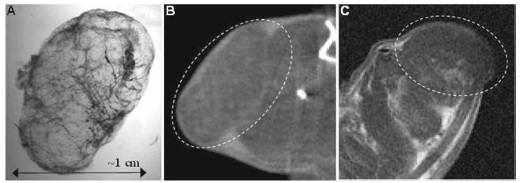
\includegraphics[scale=1]{intro_img/Oldham_2006_tumourstaining.jpg}
		\caption{Figure showing the advantage of OptCT imaging over other modalities. Part (A) shows a projection image of a HCT116 tumour after optical clearing. (B) is an \textit{in vivo} $\mu$-CT image of the same tumour with 50$\mu$m resolution. (C) is \textit{in vivo} T1 weighted contrast enhanced $\mu$-MRI image of a similar tumour. The superior resolution and contrast in the OptCT image is evident. Images  adapted from \cite{Oldham:2006}.}
		\label{fig:tumourstaining}
	\end{figure}
	
	
	
	
	
	\newpage
	\section{Conclusions}
	
	There is significant potential for further development of OptCT. Some new ideas include time-gating OPT using non-linear optics \cite{Bassi:2010}. Up-conversion using a crystal and Ti:sapphire laser  selects only ballistic light,  reducing scattering artefacts. However, employing this technique would significantly increase the system cost and complexity.
	
	Another group have successfully combined fluorescence lifetime imaging microscopy (FLIM) 
	with OPT \cite{McGinty:2008ix}. FLIM, a ratiometric modality, can provide quantitative information about the local environment around fluorophores including pH, temperature and refractive index. Protein-protein interactions can be probed using F\"{o}rster  resonance energy transfer (FRET) which can be measured using FLIM.  The set-up for FLIM-OPT is very similar to OPT and  a mathematical model is required to calculate fluorescence lifetimes from projection data. Projections are recorded for a series of time-delays for each angle. \textit{In vivo} FLIM OPT has also been reported \cite{McGinty:2011vm}, and these methods could possibly be very useful for drug screening, espcially using FRET. The authors note that using a modulated CMOS camera and sinusoidally varying LED source could be a cheaper way of implementing FLIM-OPT \cite{McGinty:2011vm}.
	
	Other improvements include the development of a computational techniques leading to increased sensitivity \cite{Hornblad:2011fh}. This is an adaptation of histogram equalisation, an established technique.
	The modulation transfer function (MTF), commonly used in optics as a measure of resolution, has been used to improve filtered in FBP \cite{Chen:2012}.
	An established technique of high dynamic range imaging has been applied to OptCT on several occasions and most recently by Fei \textit{et al.} in 2012 \cite{Peng:2012wi}.
	
	A potentially improved version of OptECT has been reported by Lorbeer \textit{et al.} in 2011  \cite{Lorbeer:2011}. A first generation scanning laser set-up is used to record fluorescent signal giving a hundredfold increase in photon collection efficiency over CCD-based set-ups. 
	
	The  biological benefits of all these new techniques have not been fully explored and there is still plenty of scope for improving this new modality.  Overall, it appears OptCT could be the ideal modality to help us understand the biological origin of contrast in MR images. Although OptCT itself will probably never be used clinically, due to the limit on sample sizes, we hope that it can help increase the usefulness of MRI. There is also potential for OptCT to be used in pre-clinical screening of drugs and in monitoring tumour progression. Especially exciting is the possibility of using fluorescent proteins to track interactions between tumour and host cells. 
	
	



	\chapter{Methods and Characterisation}

\section{Optical CT Materials and Methods}
\subsection{Hardware}

Our  optical CT system is area-detector based, allowing for fast 3-D scanning. A high quality scientific Complementary Metal-Oxide Semiconductor (CMOS) camera (Zyla sCMOS, Andor Technology PLC, Belfast, UK) has excellent sensitivity, read-out noise and fast read-out speed. 

We have two illumination sources. A flat-panel red Light Emitting Diode (LED) 
(PHLOX-LEDR-BL-100x100-S-Q-1R-24V, Phlox, Aix-en-Provence, France), with a wavelength of 633nm provides uniform lighting appropriate for imaging PRESAGE\texttrademark , a radiochromic plastic which has a strong absorption peak at 632nm. 
For tissue imaging the wavelength most appropriate for each sample is provided through the use of a  new broadband white light source (SugarCUBE LED Illuminator, Nathaniel Group Inc., VT, USA) and tunable filter (VariSpec, PerkinElmer, Inc., MA, USA). 

	\begin{figure}[H]
		\centering
		\subfigure[System setup diagram]{\label{subfig:setupdia}
			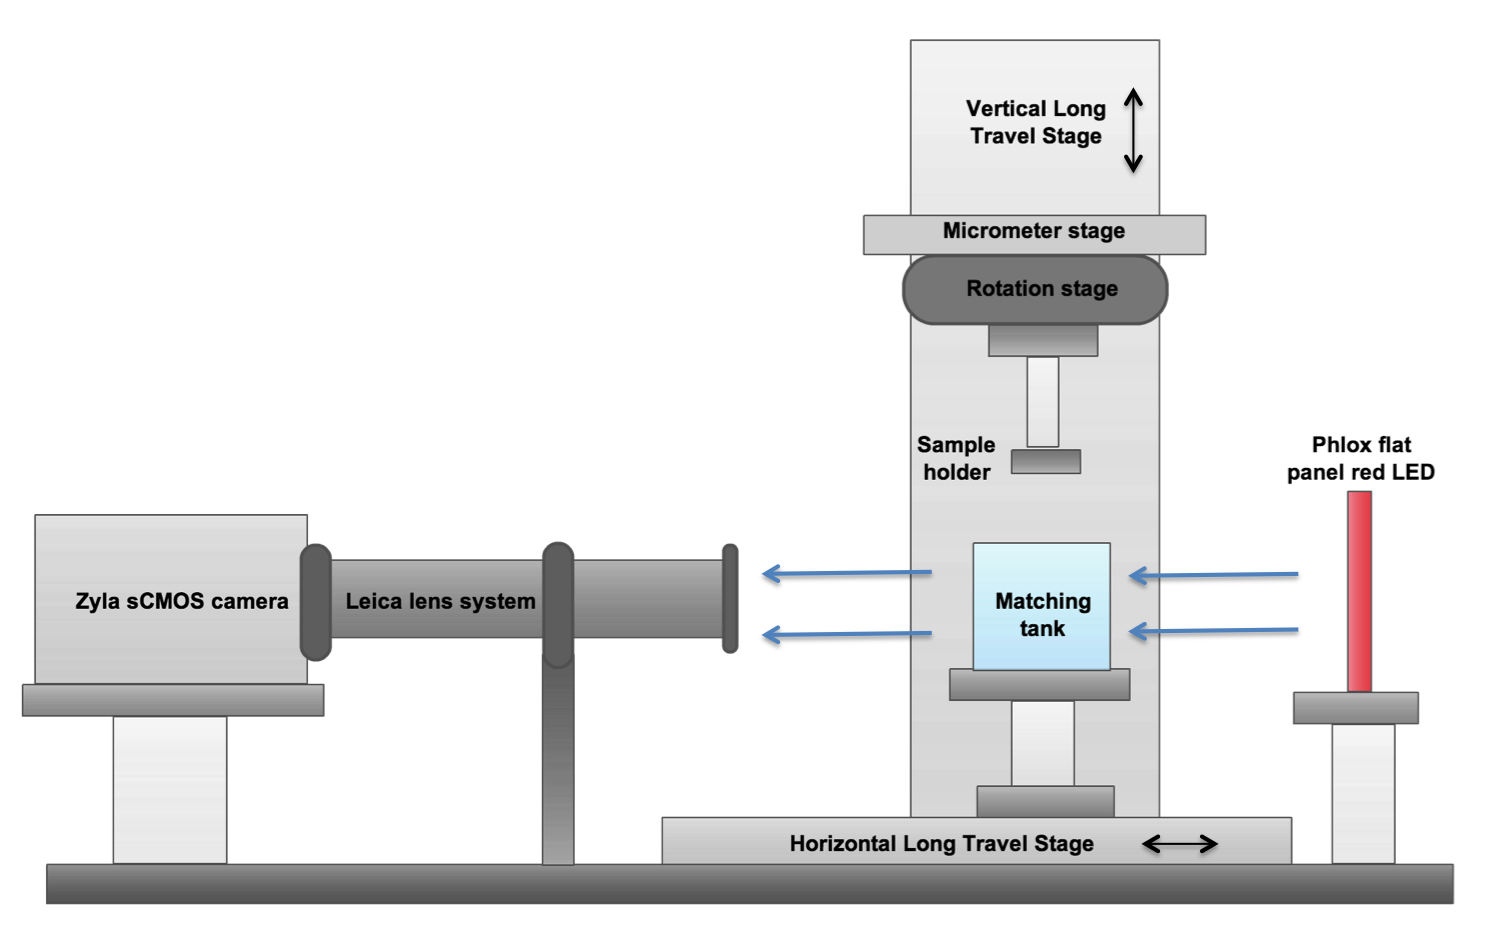
\includegraphics[width = \textwidth]{meth_img/setup_diagram.png}}
		\subfigure[System setup photo]{\label{subfig:setupphoto}
			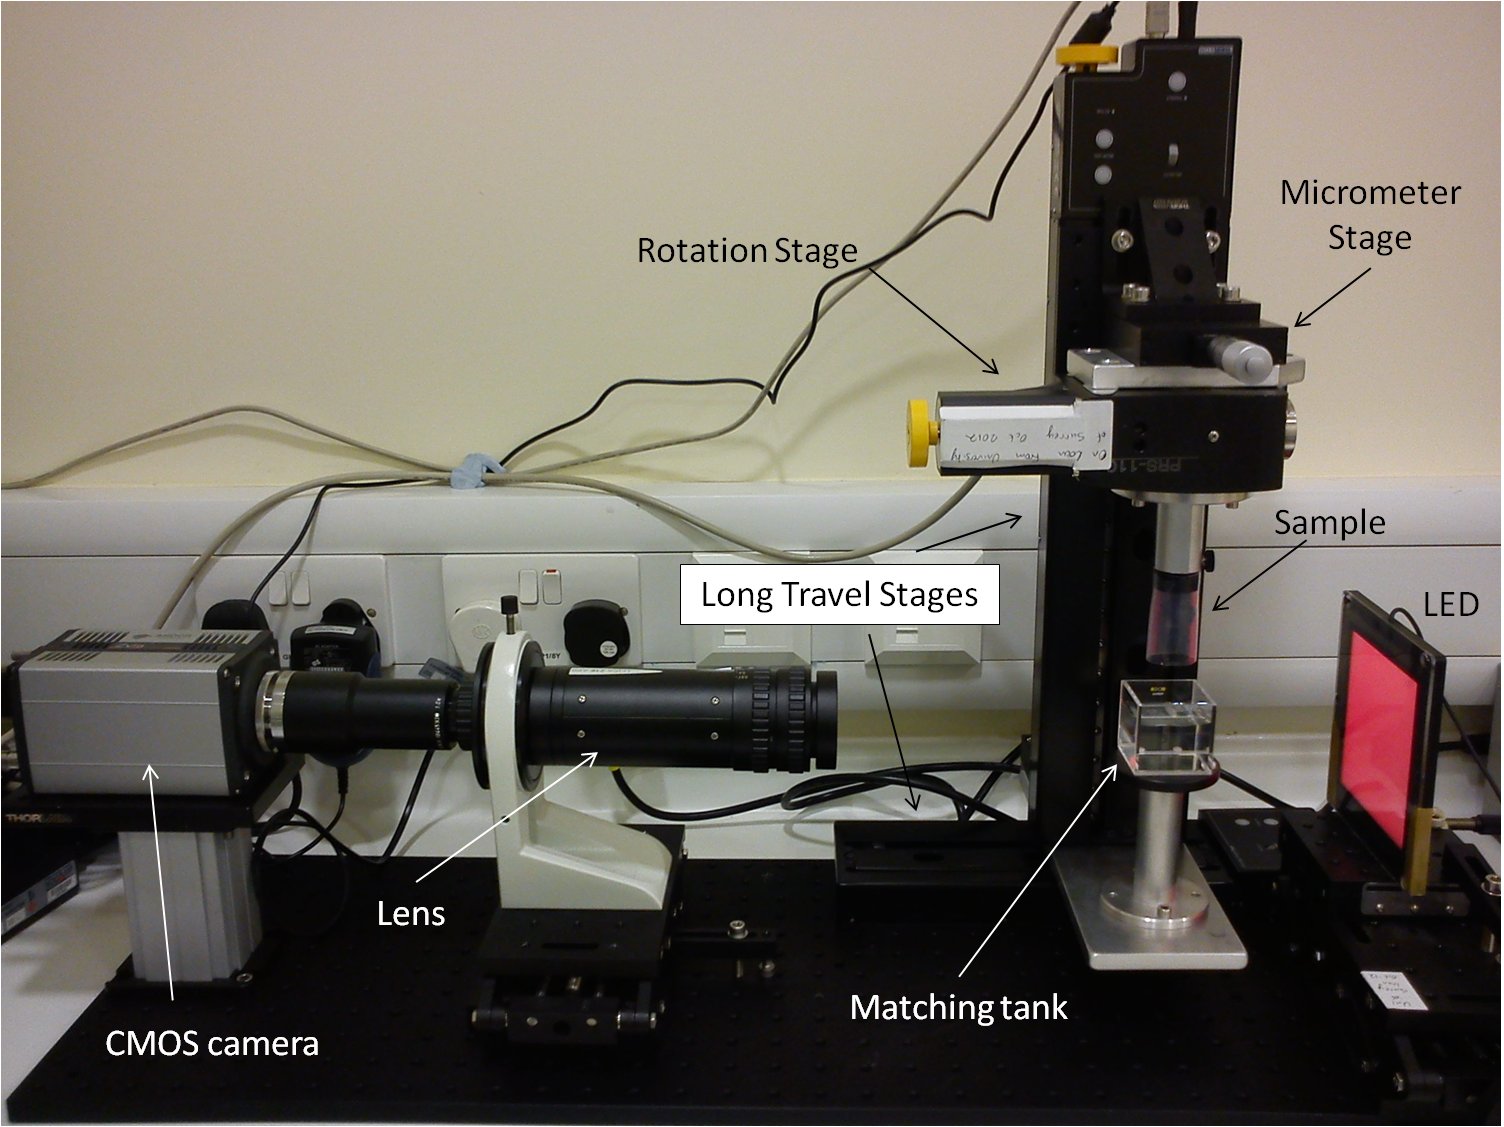
\includegraphics[width = 0.85\textwidth]{meth_img/Tidy_setup.png}}
		\caption{Diagram and picture  of current set-up of optical CT system at the ICR with principal parts of apparatus labelled.}
		\label{fig:setup_pic}
	\end{figure}

Samples are suspended from a rotary stage (PRS-110 ZSS43, PI miCos GmbH, Eschbach, Germany) in a glass matching tank (Part 704-002-40-10, Hellma GmbH, M\"{u}llheim, Germany). The COR can be adjusted through a micrometer stage which moves the rotation stage. A COR-checker LabView program checks for accurate alignment of the COR with the centre of the FOV. Off-centre COR leads to artefacts which can be corrected as part of the reconstruction.

The matching tank is filled with `matching liquid' with an RI close to that of the sample, avoiding refraction at the curved surface of the sample. For PRESAGE samples this matching fluid was a solution of (97\% ethyl hexyl salicylate and 3\% 4-methoxycinnamic acid 2-ethylhexyl ester) giving the same refractive index as the PRESAGE\textregistered. The clearing solution used for each tissue sample was used for matching fluid.

For initial measurements  the rotation stage was supported on a large optical post. In an updated system this post was replaced with an Integrated Long Travel Stage (LTS-300/M, Thorlabs Ltd., Ely, UK ) which allows  accurate and reproducible vertical positioning of samples. 
In collaboration with the ICR workshop, a novel mounting system has been developed to give reproducible positioning of samples allowing pre and post-irradiation scans of dosimetry gel. 
Two custom sample mounts are used for dosimetry and tissue samples respectively. The dosimetry mount fits caps that are fixed to PRESAGE samples, meaning the samples are in the same orientation for every scan. The tissue mount has two additional stages, giving the flexibility to position irregular samples on the COR independently of moving the COR.  

An additional Long Travel Stage (LTS-150/M, Thorlabs LTD., Ely, UK ) allows accurate positioning of the sample and tank along the optical axis.  

Light is collected by an imaging lens system made up of  components of the modular `Z16 APO' zoom system  (Leica Microsystems GmbH, Wetzlar, Germany, see \cite{Doran:2010hn} for details). The use of the zoom lens allows manual adjustment of the focus and magnification. However, in general the manual focus is left constant and we use the LTS stage to move the sample and tank along the optical axis for focusing - more repeatable. Add focusing protocol.








\subsection{Software}
\subsubsection{Acquisition}

Image acquisition and rotation are controlled synchronously  by PC using an in-house program written in LabView (National Instruments Corporation Ltd., Berkshire, UK). The high capacity of the PC and camera allows for fast read-out of images giving much reduced scan times to others previously reported. For standard scans  images are acquired during continuous rotation of the sample. 

If projections are acquired with no binning then a Step-and-shoot method with averaging of several projections is used to improve the SNR. This method takes much longer.

Include algorithms? Maybe in appendix?




\subsubsection{Reconstruction}
Reconstruction is carried out via Filtered Back-projection (FBP) incorporating a `correction scan' using in-house software  written by  SJD in IDL (Excelis Visual Information Solutions, Boulder, CO) (see \cite{doranestablishing2013}). 
%Shepp-Logan filter used?




`Dark' field (DF) and `light' field (LF) images correct for structural noise in the camera and non-uniformities in the light path respectively. In general 30 DF (with cap on camera) and LF (no sample present) images were averaged for each scan and images are corrected during reconstruction according to  equation (4) of Krstaji\'{c} \cite{Krstajic:2007ec}.  

The software also allows for adjustment to correct for off-axis  centre of rotation (COR). In the updated system  the rotation stage is mounted on a micrometer stage allowing more precise alignment of the CoR. If the CoR is not aligned with the central pixel column then the sample will appear to drift across the screen and projection data will not be consistent for all angles. \cite{Oldham:2006b}

A ring artefact correction has been added to the reconstruction, based on [INSERT reference]. The number of pixels can be chosen depending on the matrix size of the projections.


\subsection{Dosimetry protocol}


Optical CT imaging of PRESAGE samples was carried out in two modes.
For qualitative visualisation of irradiation patterns fast scans were used, while samples for PVDR assessment were scanned with high-resolution scans. All scans had an aperture setting of A=1 so that the DOF encompassed the entire sample.


		
	\begin{table}[H]
		\centering
		\begin{tabular}{ p{2.3cm}  p{2.5cm} p{2.5cm}  p{2.3cm} p{2.5cm}  }
			\hline
			\textbf{Scan} & \textbf{Projections} &\textbf{Pixels}   &\textbf{Voxel size ($\mu$m)} & \textbf{Acquisition time} \\ \hline 
			Fast  & 1000 & $512\times 512$  & 20.8 &2.5 minutes \\ %\hline
			High-resolution & 3200 & $2048\times 2048$ &  5.2 & 1 hour \\ 
			\hline
		\end{tabular}
		\caption{Different scanning parameters for MRT}
		\label{table:scansettings}
	\end{table}
	
	
	

	\begin{figure}[H]
		\centering
		\subfigure[Projection 190]{\label{subfig:presageproj1}
			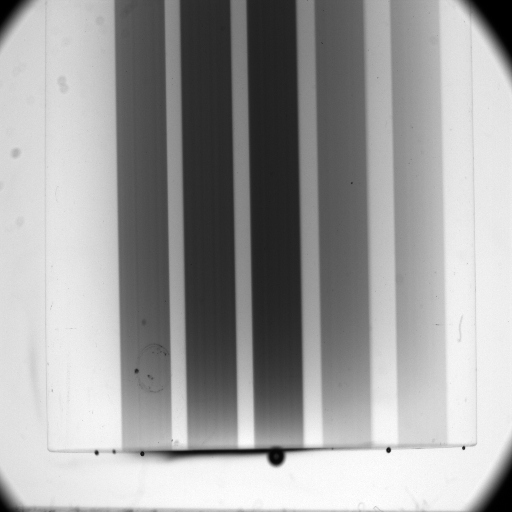
\includegraphics[width=0.45\textwidth]{meth_img/P19_proj_190.jpeg}}
		\subfigure[Projection 690]{\label{subfig:presageproj2}
			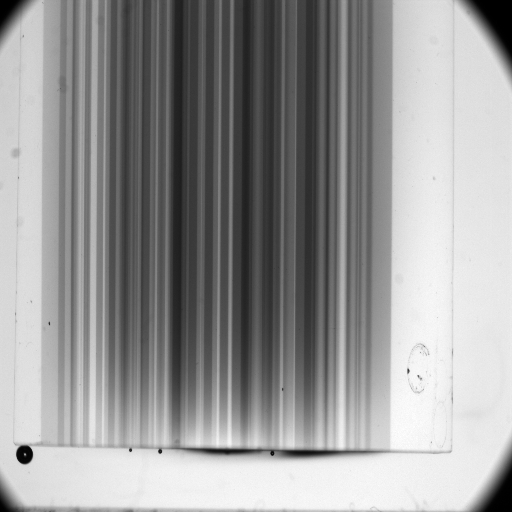
\includegraphics[width=0.45\textwidth]{meth_img/P19_proj_690.jpeg}}
		\caption{Projections taken $180^{\circ}$ apart through a PRESAGE\texttrademark ~sample irradiated at the ESRF with a defined test pattern of known line widths. Some air bubbles can be seen as dark circles at the base of the sample. Faint marks in the upper left parts of the images are caused by dust in the optics which will be corrected by a Light Field scan. In \ref{subfig:presageproj2} a mark on the side of the sample itself can be seen near the bottom right. A small refractive index mismatch between the sample and liquid is seen by the faint outline of the sample walls. This will result in a circular artefact in reconstructed slices.  }
		\label{fig:presage_projections}
	\end{figure}



Projections, such as those seen in Figure ~\ref{fig:presage_projections} were reconstructed to give slices through the sample. A view through the sample made up of 20 averaged slices is seen in Figure~\ref{fig:presage_slice}. It was possible to average slices and thereby improve the SNR of the image because the sample was axially uniform. A clear dose pattern can be seen in the sample, similar to those previously reported by Doran \textit{et al.} \cite{doranestablishing2013}. Some blurring and ring artefacts can be seen but the overall  image quality is good with high SNR. The RI mismatch artefact is not significant but could be improved. Lineprofiles for each row numbered on the slice are shown in Figure~\ref{fig:P19_lp} showing how the system response falls off with increasing line-pairs per mm (lppm).  A rolling baseline as previously reported by Doran is seen for line 3 whereby the signal falls off towards the edges of the sample.  The highest lppm pattern resolved was 20 lppm, seen  on the far left of line 4. Three patterns on line 4 were not resolved representing 30, 40 and 50 lppm. This means the smallest resolvable object was between 66-$100\mu m$ and not  $40\mu m$ as predicted by the MTF data. This discrepancy is probably due a combination of blurring due to reconstruction, imperfect focusing and the fact that projections of the patterns are not always acquired with the pattern in the centre of the focal plane.  
The results from this phantom verified the optical CT system was working for dosimetry, allowing us to move onto adapting the system for imaging tissue. 



	\begin{figure}[H]
		\centering
		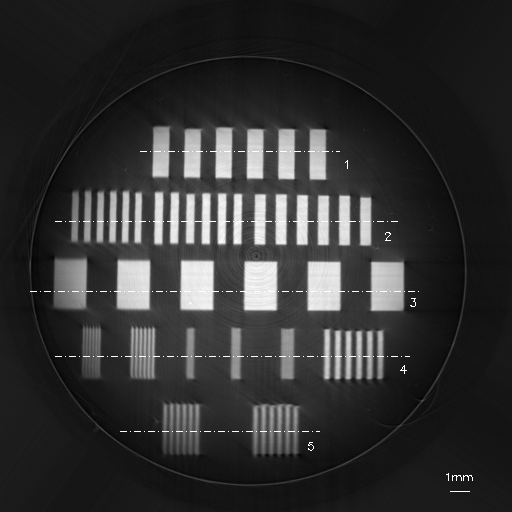
\includegraphics[width=0.72\textwidth]{meth_img/P19_recon370-399av_lineprofiles.png}
		\caption{Reconstructed slice of the PRESAGE\texttrademark ~sample seen in Fig.~\ref{fig:presage_projections}. The image is a result of 20 averaged slices to improve the SNR. Annotations refer to line profiles plotted in Fig.~\ref{fig:P19_lp}. }
		\label{fig:presage_slice}
	\end{figure}
	
	\begin{figure}[H]
		\centering
		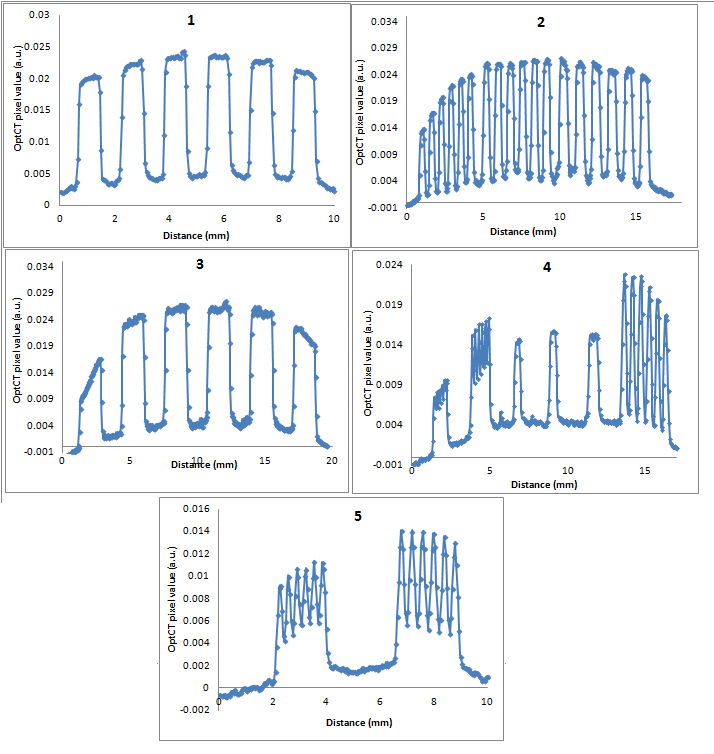
\includegraphics[width=\textwidth]{meth_img/P19_lineprofiles.png}
		\caption{Lineprofiles for PRESAGE\texttrademark ~sample shown in Figure~\ref{fig:presage_slice}. The highest resolution pattern resolved was 20 lppm (far left of pattern 4) but  the 30, 40 and 50 lpppm patterns on line 4 are unresolved. No modulation is seen for these patterns indicating that objects smaller than $100\mu m$ cannot be imaged.}
		\label{fig:P19_lp}
	\end{figure}




\subsection{Tissue imaging protocol}



Before imaging, tissue samples must undergo a series of preparation steps:
\begin{itemize}
	\item Fix in $70\%$ ethanol in phosphate-buffered saline (PBS) overnight
	\item Embed in $0.75\%$ agarose for stability
	\item $3-4$ washes of $100\%$ ethanol
	\item Washes of $30\%$ and $70\%$ 1:2 benzyl benzoate:benzyl alcohol (BABB) in ethanol
	\item $1-2$ washes of $100\%$ 1:2 BABB (refractive index 1.559)
	\item Superglue agarose to sample holder prior to imaging with 1:2 BABB matching fluid.
\end{itemize}



Due to the small size and irregular shapes of tissue samples, a new positioning system was necessary to allow flexible positioning of samples on the centre of rotation. This is coupled with a LabView program for alignment makes sample positioning much easier, previously difficult and time consuming. 




	\begin{figure}[H]
		\centering
		%	\subfigure[Clearing heart]{\label{subfig:clearingheart}
		%		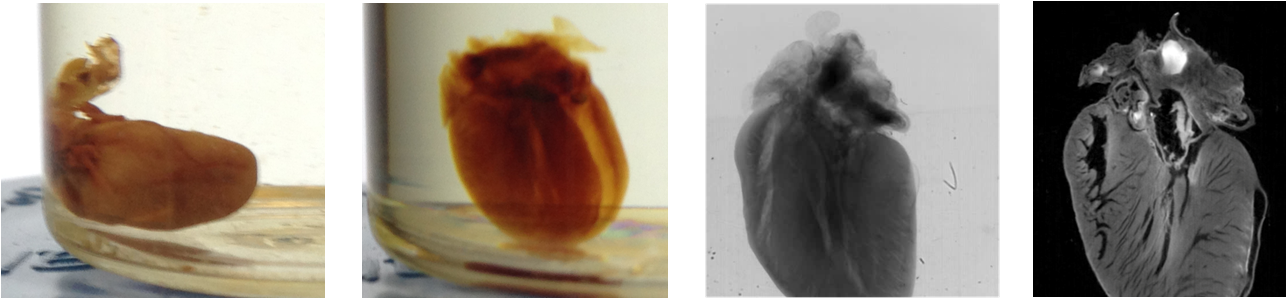
\includegraphics[width = \textwidth]{clearing_process_heart.png}}
		%	\subfigure[Clearing brain]{\label{subfig:clearingbrain}
		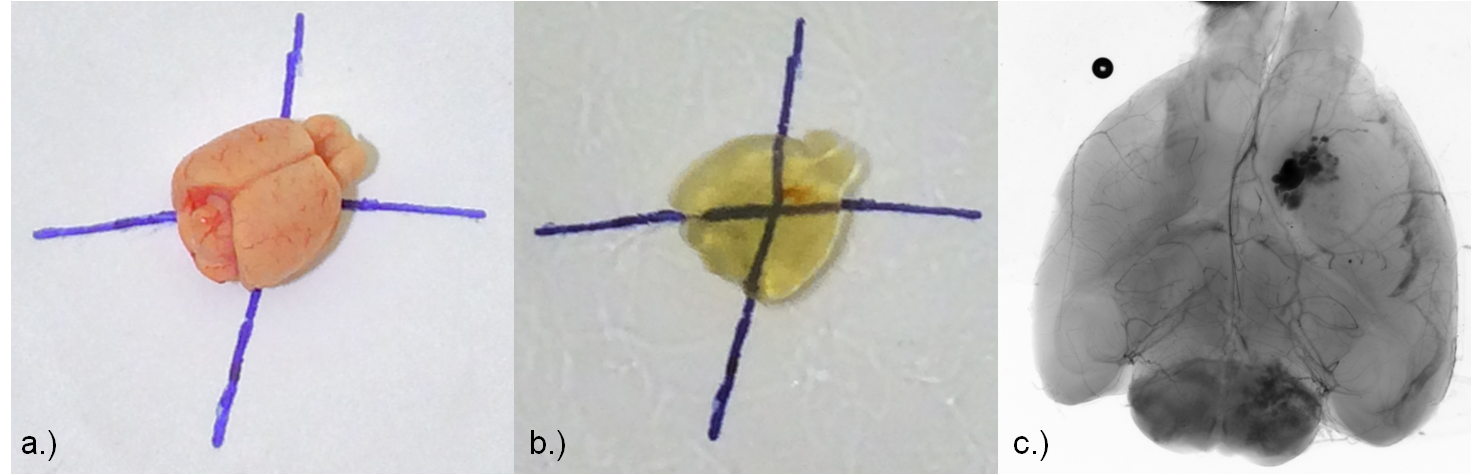
\includegraphics[width = \textwidth]{meth_img/Brain_J5_clearing.png}
		\caption{a.) Example of an uncleared mouse brain, b.) a cleared mouse brain in 1:2 BABB solution, c.) a projection image of the cleared brain mounted in the optical CT system.}
		\label{fig:clearing}
	\end{figure}




%\begin{figure}[H]
%	\centering
%	\subfigure[System setup photo]{\label{subfig:tissuesetupphoto}
%		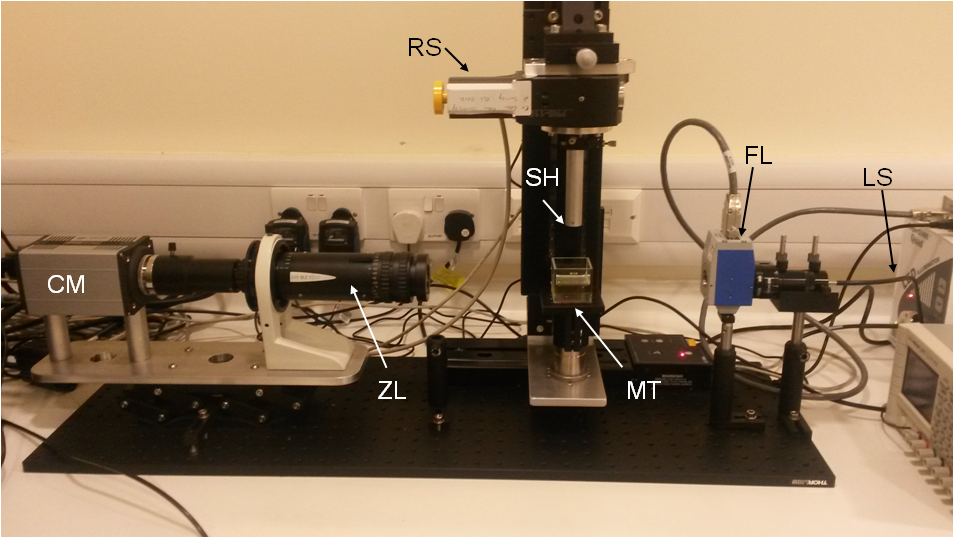
\includegraphics[width = 0.85\textwidth]{Tissue_set-up.png}}
%	\caption{Diagram and picture  of current set-up of tissue OptCT system at the ICR with principal parts of apparatus labelled. Add pictures of sample preparation.}
%	\label{fig:tissuesetup_pic}
%\end{figure}



Examples images of different healthy rodent organs are shown in Figure~\ref{fig:heart_brain}. Clearing with BABB has worked well and all contrast is endogenous. Clearing reduces light attenuation due to scattering, so any contrast is due to natural differences in light absorption properties between different tissue types. Highly attenuating areas, such as haemoglobin in the heart, or lipid-dense areas of the brain, are bright in these optical CT absorption scans.

Images of tissues containing tumours are shown in Figure~\ref{fig:tumours}, ranging from a large neuroblastoma tumour, of the order of 10mm, to a tumour cell spheroid around $100\mu$m diameter, at the extreme resolution limit of the system. It was noted that large and highly attenuating tissues (such as neuroblastoma tumours) required longer clearing time.


	\begin{figure}[H]
		\centering
		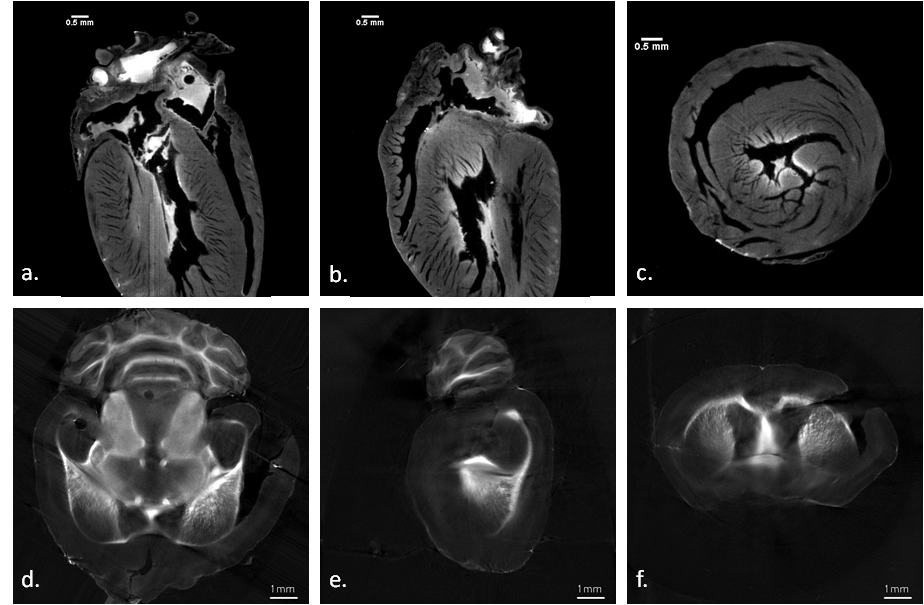
\includegraphics[width = \textwidth]{meth_img/heart_brain_sclbr.png}
		\caption{a-c.) Orthogonal slices of a reconstructed image volume of a mouse heart with endogenous contrast, most likely due to the presence of haemoglobin. d-f.) Orthogonal slices of a reconstructed image volume of a mouse brain where bright areas are likely due to attenuation due to lipid content of the brain. These images demonstrate high-resolution, highly detailed data reconstructed from absorption optical CT scans,  without addition of external contrast.}
		\label{fig:heart_brain}
	\end{figure}
	
	\begin{figure}[H]
		\centering
		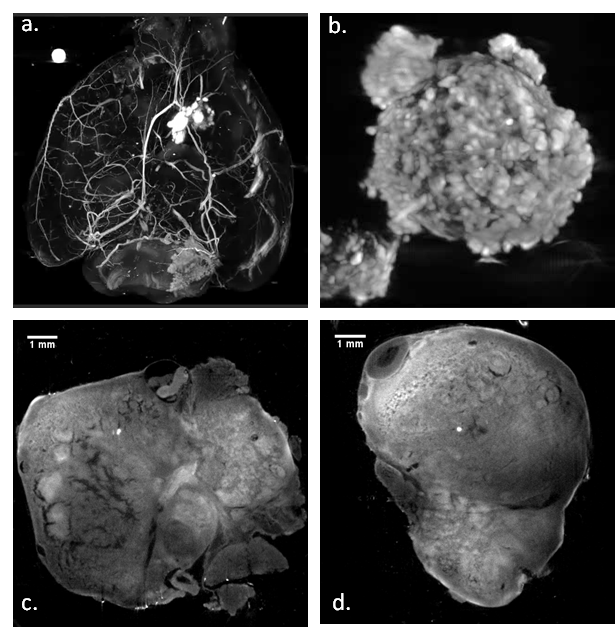
\includegraphics[width = \textwidth]{meth_img/tumours.png}
		\caption{a.) Maximum intensity projection (MIP) of a mouse brain with an orthotopic glioblastoma tumour. A highly attenuating artefact due to an air bubble is seen in the top left corner. The mouse was injected with Evans Blue, an absorbing permeability marker which has stained the vasculature. The tumour was rich in haemoglobin and also appears very attenuating. This shows the potential for optical CT imaging of vasculature. b.) MIP image of a tumour cell spheroid stained with haematoxylin. c-d.) Orthogonal slices through a neuroblastoma tumour showing the detail possible using an anatomical scan. Additional functional information can be added with the use of fluorescent markers. }
		\label{fig:tumours}
	\end{figure}









\section{Optical CT system characterisation}

\subsection{Linear response}

In order to establish the relationship between optical CT reconstructed pixel value and optical absorbance,  gel finger phantoms were made in a similar fashion to \cite{Oldham:2003}.  

10\% porcine gelatin (Sigma, REF) was made in water. Add exact method? Maybe in appendix. Heat to 60?deg, vacuum, stir while cooling to 25?. 

A specialised finger phantom mould was made by the ICR workshop. A 3-D printed holder contained slots to hold metal rods on one side and can be attached directly to the rotation stage on the other. A cylinder of Teflon FEP heat-shrink plastic (Holscot Fluoroplastics Limited, Grantham, UK) was used to provide support for the gelatin. Teflon FEP has an RI of 1.341  making it a very close match for water and gelatin. \cite{Krstajic:2006kna} Cylindrical pieces of Teflon sleeving were cut a length of 4cm, the height of the matching tank and one end was heat shrunk onto the plastic mould providing a secure support for the cooling gelatin. It was important to make sure the Teflon sleeving was not too tight around the plastic mould, if no air can come through the bottom then the metal rods cannot be removed easily creating air-bubbles leading to attenuation artefacts. Three removable metal rods were placed in each mould.


Clear gelatin was allowed to set at room temperature around the metal rods, which  were then carefully removed.  Evans Blue (T-1824), an azo dye which is both optically absorbing and  fluorescent, was used to provide optical contrast. Small amounts of Evans blue were added progressively to gelatin which was kept at 30deg using a heater-stirrer. The Evans blue doped gelatin was injected into the inclusions left by the metal rods using a 1ml syringe. A cuvette of each concentration of Evans blue gelatin  was filled and allowed to set. The optical absorbance of each cuvette was measured using a spectrophotometer (REF). Phantom A had 3mm diameter inclusions and phantom B, 2mm inclusions, with increasing Evans Blue concentrations.

The phantoms were scanned under the same imaging conditions. The matching liquid used was 4.5\% salt solution (RI $\approx 1.341$) which  gives a closer refractive index match than water. The average reconstructed pixel value of each finger was calculated from a single axial slice and averaged over a $25 \times 25$ pixel area within the inclusion (see Figure~\ref{fig:fingerphantoms_roi_EB}b).
As can be seen in Figure~\ref{fig:fingerphantoms_roi_EB}c, the reconstructed pixel value of the optical CT system is linearly related to the optical absorbance as measured by  spectrophotometer.   The use of two phantoms verifies the linear relationship and the repeatability of measurements.  

	\begin{figure}[H]
		\centering
		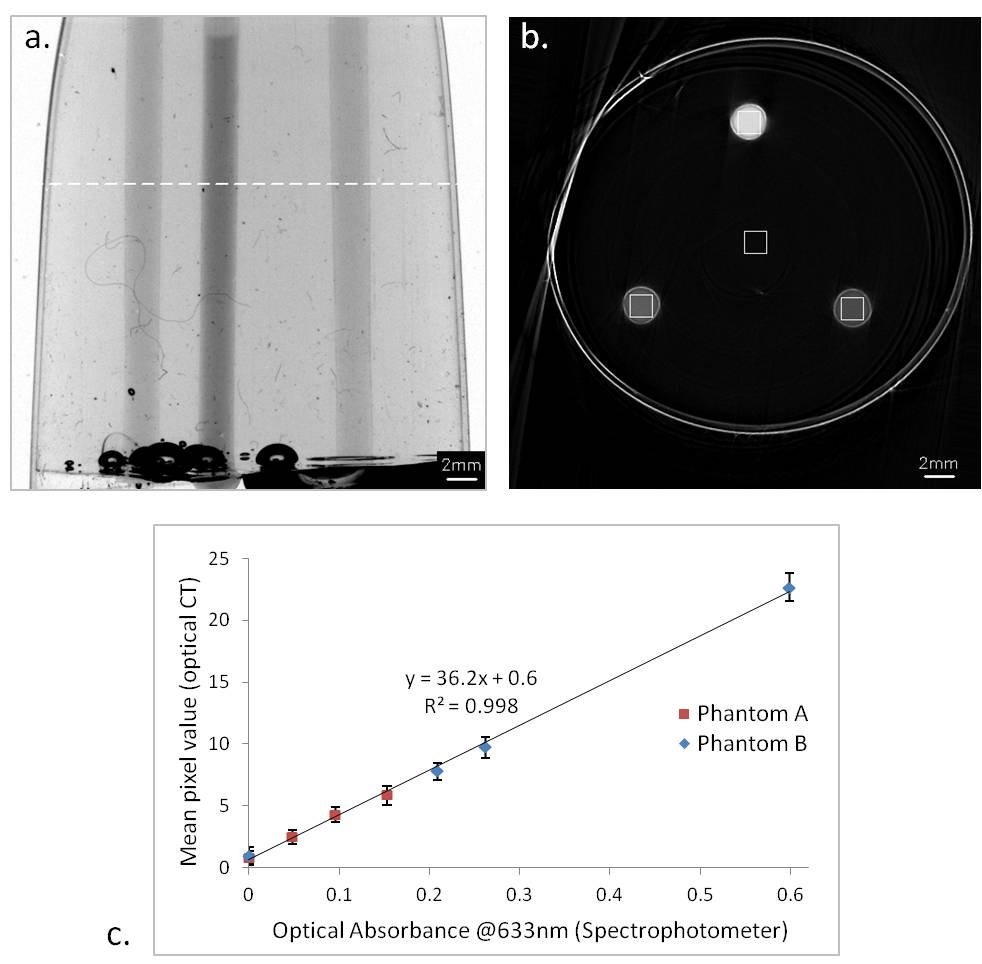
\includegraphics[width=1\textwidth]{meth_img/EB_rod_new.jpg}
		\caption{a. An optical CT projection image of a gelatin phantom containing `finger' inclusions of different concentrations of Evans blue-dyed gel. b. A reconstructed slice through the phantom in the axial position marked by the dashed line in (a). Regions of Interest (ROIs) mark where the mean pixel value was calculated for each finger and the clear gelatin. The double ring artefact is due to refractive index mismatch between gel and the Teflon FEP container, and also between the Teflon and 4.5\% saline solution matching liquid. c. Plot of absorbance of Evans Blue-doped gel measured with a Spectrophotometer against mean pixel value of different regions on reconstructed optical CT images. Two phantoms were measured  with all  variables constant between readings.}
		\label{fig:fingerphantoms_roi_EB}
	\end{figure}
	



We expected that once the absorbance is too high the system response will drop off non-linearly due to a lack of photons. This was demonstrated with a PRESAGE sample containing very large doses of radiation. Show graph of L3?






\subsection{Spatial resolution}

\label{subsubsec:MTF}

Understanding the spatial resolution response of the optical CT system is very important for acquiring high-quality, quantitative images. 
Previous publications noted a reduction of optical CT image contrast of small features as the feature size approaches the resolution. \cite{doranultra-high2013} This effect is evident even when the feature size is several times the nominal spatial resolution and leads to non-linear response to optical absorbance. Therefore, the limits of spatial resolution of the system must be carefully characterised before we can be confident that measurements are quantitative. 

There are many factors which can affect optical CT resolution (see theory section?). There is an added complexity when imaging extended objects as standard microscope lenses are designed to image a thin sample at the focal plane. For optical CT the spatial resolution either side of the focal plane is important as ideally the entire sample should be in focus at all times (see Figure~\ref{fig:idealdof}). The distance over which the focus is `acceptable' is known as the depth-of-field (DOF).

\begin{figure}[H]
	\centering
	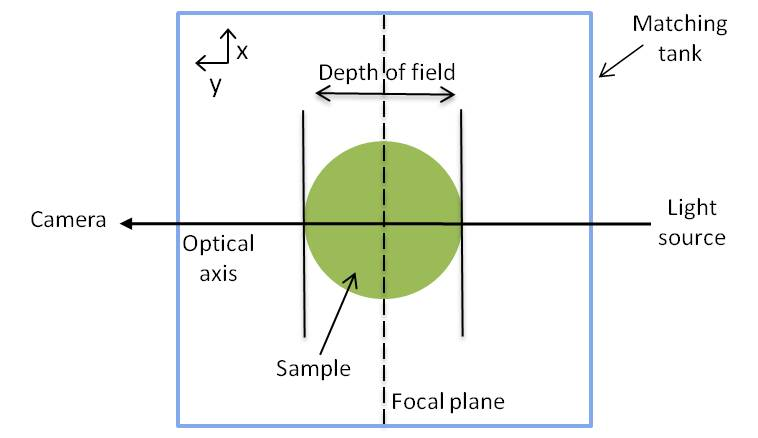
\includegraphics[width=0.9\linewidth]{meth_img/ideal_dof_diagram}
	\caption{Schematic of the optical CT system geometry showing the ideal positions of the focal plane and depth-of-field.}
	\label{fig:idealdof}
\end{figure}

Our optical system consists of components from a modular microscope system. This includes a zoom lens, giving variable magnification settings, and a variable aperture which controls the DOF of the system. 
The aperture size can determine the overall acceptance angle of the optical system, $\theta$, which in turn affects the numerical aperture (NA), defined as $N_A = n \sin{\theta}$.  A system with high NA results in high resolution, $\Delta x$ (Equation~\ref{eqn:airy}). However, such a system has a small DOF due to the inverse relationship between DOF and NA (Equation~\ref{eqn:dof}).
\begin{equation}
\Delta x =  \frac{0.61 n\lambda}{N_A}
\label{eqn:airy}
\end{equation}
\begin{equation}
\mathrm{d_{DOF}} = n_{bath}\left( \frac{n\lambda}{N_{A}^2}+\frac{ne}{MN_{A}} \right) = \frac{n_{bath}}{0.61n\lambda}\left( \Delta x^2 + \frac{n e}{M}\Delta x \right)
\label{eqn:dof}
\end{equation}
where $n$, the refractive index of the medium around the lens, $n_{bath}$ the refractive index of the medium surrounding the sample, $M$ the lateral magnification of the system, $e$ the pixel size of the camera and $\lambda$, the wavelength of light.





To investigate the effect of changing the NA of our system we measured the modulation transfer function (MTF) for a range of positions along the optical axis. Five different NA values were evaluated, corresponding to the five reproducible aperture size settings on the lens system, labelled as A=1 to A=5, with A=1 being the smallest aperture and A=5 being the fully open aperture setting. 

The modulation transfer function (MTF) characterises the resolution of a system by measuring how different spatial frequencies are transmitted.
It is the Fourier transform of the Point Spread Function (PSF), giving a more comprehensive description of an optical system than quoting a single  resolution value. There are various methods of measuring the MTF including simulating a point source or measuring the response to a sinusoidal pattern. These methods require test objects accurate to sub-pixel distances. 
It is much easier to manufacture an accurate  sharp edge rather than  a point source or slit. It has been shown that the MTF can be calculated analytically from the Edge Spread Function (ESF) as follows,
\begin{equation}
\mathrm{MTF}(f) = \mathscr{F}\left[\mathrm{LSF}(x)\right] = \mathscr{F}\left[\frac{d}{dx}\mathrm{ESF}(x)\right]
\end{equation}
where $f$ is spatial frequency, $x$ is displacement and LSF is the Line Spread Function given by the profile of a slit source. \cite{Boone:1986}

Any noise in the data is amplified  through the derivative and Fourier transform. Therefore, following the method of Boone \textit{et al.},   the MTF was calculated directly from the fit parameters of a function  fitted directly to measured ESF data. \cite{Boone:1994} Analysis was carried out in IDL  using curve fitting function `\textit{mpfit}'.  \cite{Markwardt2009mpfit}

A knife edge was positioned at the focal plane and 50 projection images of matrix size $2048\times 2048$ were acquired and averaged to improve the signal-to-noise ratio (SNR). The knife edge was moved in steps of 0.1mm away from the focal plane in both directions along the optical axis.  Images were acquired over a distance of 0.5mm in each direction giving a total distance of 1mm, the same as the FOV of each projection image. This was repeated for each aperture setting of the microscope lens.


Plotting the MTF at each position along the optical axis as an image, the DOF is visualised in a similar manner to  \cite{chenincorporation2012}. The maximum resolution for each NA was taken as the largest spatial frequency with continuous MTF values over 0.1 over some y-range, being the DOF for that resolution.


The MTF was calculated from ESF data, as seen in Figure~\ref{fig:MTFtarget},  for a range of magnifications, pixel binning and LED voltages. The results  in Figures~\ref{fig:MTF_50}  show that system response varies significantly with these variables as is expected. Magnifcations of 0.8, 1 and 8 were tested to demonstrate the worst,  standard and best conditions for imaging respectively.





The MTF was calculated from the ESF, measured across the centre of the knife-edge images, according to equation ? for each position along the optical axis and for each NA value. The MTF was represented by a grey level in a 2-D image in which the horizontal coordinate corresponds to spatial frequency, up to the desired 100mm$^{-1}$ (equivalent to a $10\mu$m line-pair), and the vertical coordinate corresponds to position along the optical axis. This allows visualisation of the DOF for each of the different NA values.
The maximum resolution and corresponding DOF were measured for each NA setting. The maximum resolution was defined as the largest spatial frequency with an MTF above 10\% at the focal plane. The DOF for this frequency was defined as the distance along the optical axis for which this spatial frequency had an MTF above 10\%.  



	\begin{figure}[H]
		\centering
		\subfigure[`Knife-Edge' Target]{\label{subfig:MTFtarget}
			
\includegraphics[width=0.3\linewidth]{meth_img/MTF3_targetimage.png}}
		\subfigure[Edge spread function from image \ref{subfig:MTFtarget}]{\label{subfig:ESF}
			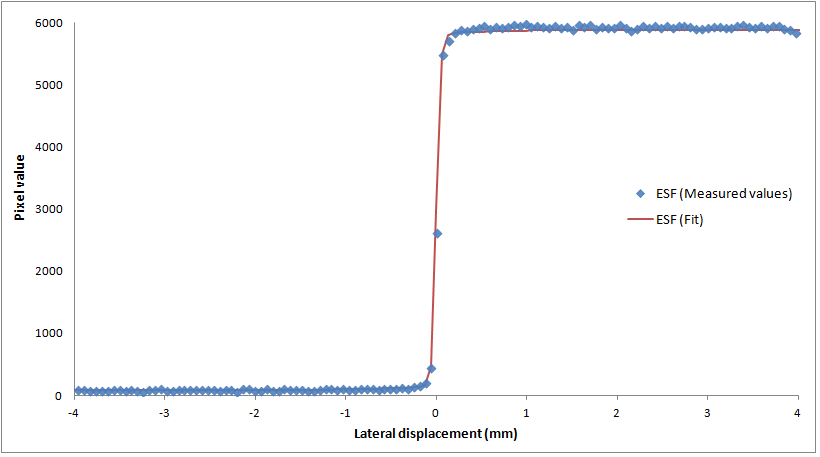
\includegraphics[width=0.55\textwidth]{meth_img/croppedESF_MTF3.png}}
		\caption{Image of a rectangular metal target with a straight edge which  approximates a `Knife' edge for the measurement of the Edge Spread Function (ESF, \ref{subfig:ESF}). The pixel row across which the ESF is measured is marked on the image. This data was cropped to give 300 points centred on the edge to allow a curve to be fitted to the data  accurately.  Pixel size was measured  allowing the pixel values to be plotted against displacement. The point of zero displacement was set at the edge for convenience in fitting a curve to the data.  The MTF is calculated directly from the ESF via  fit parameters. }
		\label{fig:MTFtarget}
	\end{figure}

	\begin{figure}[H]
		\centering
		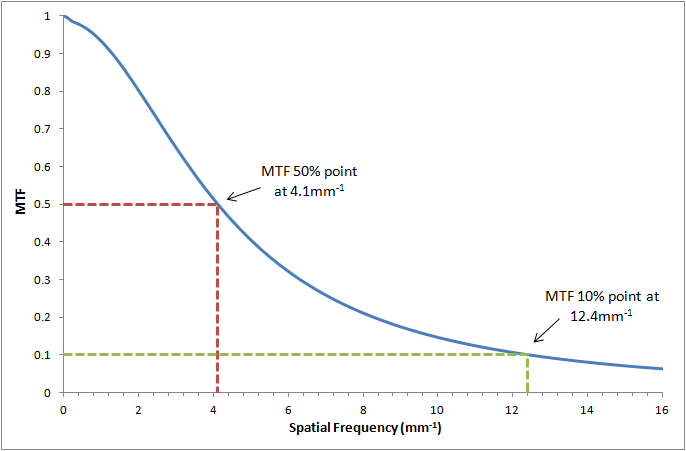
\includegraphics[width = 0.7\textwidth]{meth_img/MTF_50_graph.png}
		\caption{MTF vs spatial frequency for the case of M=1, 4x4 binning to 512x512 pixels and  LED voltage set to just below camera saturation levels, representing the imaging conditions  for most phantom images in this report. The 50\% cut-off point for the MTF, a value commonly quoted as giving the best focus is found to be $4.1mm^{-1}$. The 10\% MTF value is 12.4$mm^{-1}$ and in general this value indicates the highest  frequency that can be resolved by the system. This implies that features smaller than $40\mu m$ will not be resolved at this magnification and binning.}
		\label{fig:MTF_50}
	\end{figure}








The observed DOF and resolution results are shown in Table... and images of MTF against optical axis position are shown in Figure REF.
It is apparent that for low NA, there is a constant, low resolution across the entire FOV whereas at high NA there is a small region of high-resolution with other areas being defocused. 
%NA values in between show a sharp drop-off of DOF.





These results indicate that aperture settings must be chosen carefully for each imaging application. For most cases a constant resolution across the FOV is desirable, therefore A=1 is appropriate. For some cases, it may be desirable to have very high resolution in a small area around the centre of rotation in which case a higher aperture setting may be appropriate. However, positioning of the focal plane is very sensitive,  illustrated through the use of a `point' object test phantom containing $5\mu $m beads (Figure REF), it is apparent that the focal plane is not at the centre of the object. It is possible to attach this  bead phantom to the bottom of other samples which gives us the ability to quantify  how the resolution changes over the FOV. 



	



Ideally the DOF of projection images should be larger than or equal to the sample size, as demonstrated in Figure~\ref{fig:idealdof}. However, there is a trade-off between DOF and resolution,  $\Delta x$, given by \cite{inoue1997video} as follows,
\begin{equation}
DOF = \frac{n_{bath}}{0.61 n \lambda} \big(\Delta x^2 + \frac{ne}{M_{lat}} \Delta x \big)
\label{eqn:1DOF}
\end{equation}
where, $n_{bath}$ is the refractive index of the medium surrounding the sample, $n$ is the refractive index of the medium around the lens, $\lambda$ is the wavelength of light, $e$ is the pixel size of the camera and $M_{lat}$ is the lateral magnification of the system. The DOF of the system can be adjusted by adjusting the overall acceptance angle of the system, $\theta$, which in turn controls the numerical aperture (NA) and this is inversely proportional to the resolution, 
\begin{equation}
NA = n \sin \theta = \frac{0.61n\lambda}{\Delta x}
\label{eqn:2NA}
\end{equation}



	\begin{figure}[H]
		\centering
		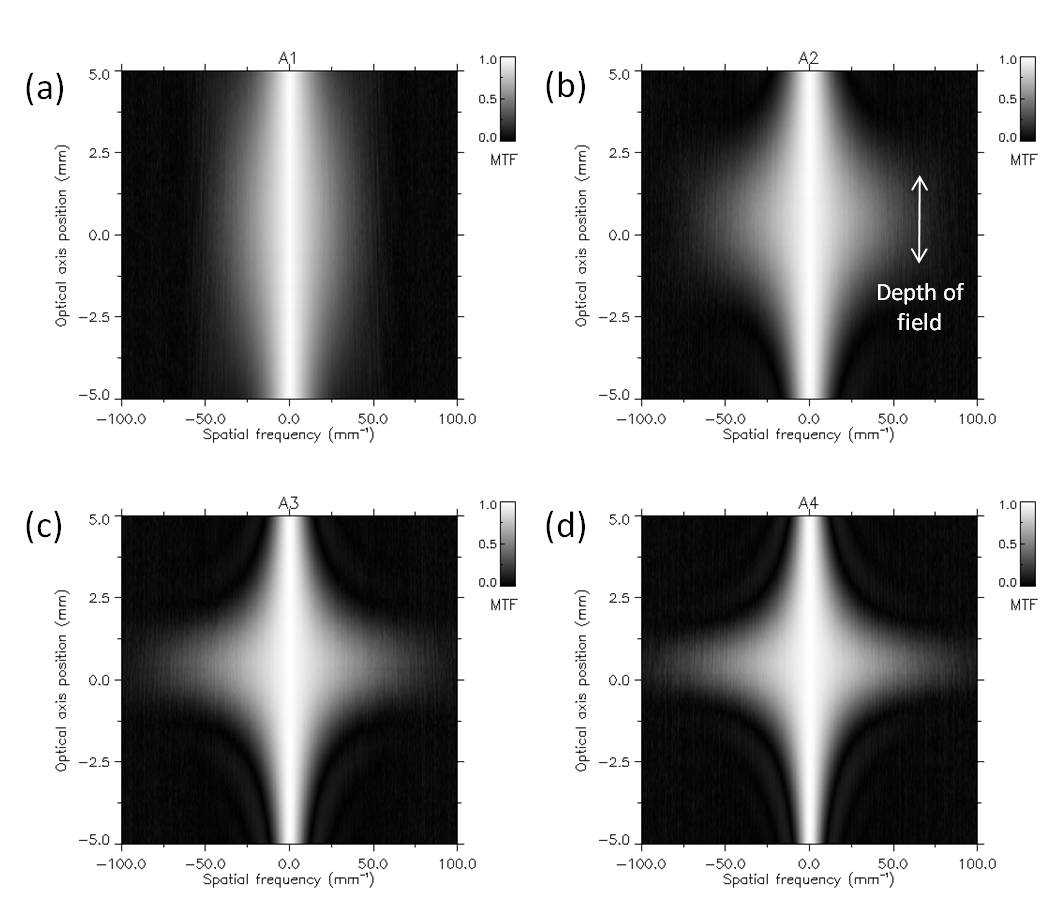
\includegraphics[width=0.9\linewidth]{mrt_img/mrt_Fig6}
		\caption{Measurements of the modulation transfer function (MTF) along the optical axis for different numerical aperture (NA) settings of the system, (a) A1 (b) A2 (c) A3 (d) A4. This allows visualisation of the depth-of-field (DOF).}
		\label{fig:MTFDOF}
	\end{figure}
	
	\begin{table}[H]
		\centering
		\begin{tabular}{ p{2.5cm}  p{3.5cm} p{4.5cm}  }
			\hline
			\textbf{NA setting} & \textbf{Resolution ($\mu$m)} &\textbf{Depth of field (mm)}  \\ \hline
			A1  & $21.5 \pm 0.5$ & $9.3 \pm 0.4$ \\ %\hline
			A2  & $13.7 \pm 0.1$ & $2.4 \pm 0.2$ \\ %\hline
			A3  & $12.0 \pm 0.2$ & $1.6 \pm 0.2$ \\ %\hline
			A4  & $10.1 \pm 0.2$ & $0.6 \pm 0.1$ \\ %\hline
			A5  & $9.7 \pm 0.2$ & $0.4 \pm 0.1$ \\ \hline		
		\end{tabular}
		\caption{Maximum resolution and corresponding depth-of-fields for different NA settings on the optical CT system. The uncertainties reflect noise in the modulation transfer function (MTF)  measurements.}
		\label{table:DOFNA}
	\end{table}



These measurements were all taken in `projection' space and do not take into account the effect of the reconstruction process on resolution. 

Bead phantom construction. A=5, m=8, sum 50 slices to get good visualisation

\begin{figure}{H}
\centering
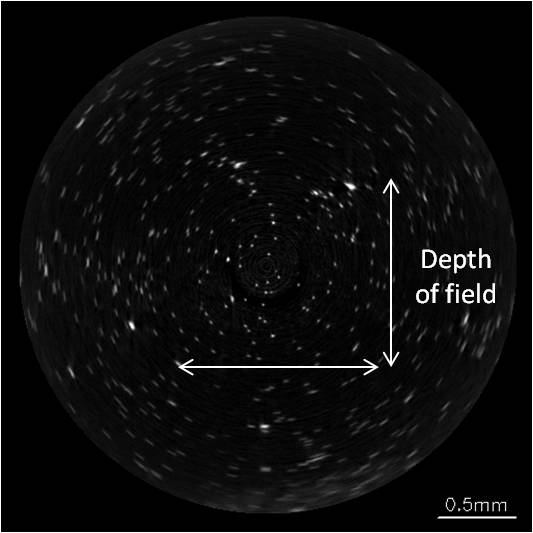
\includegraphics[width=0.7\linewidth]{meth_img/bead_DOF_d2_res_test_1_10_15_scan5.jpg}
\caption{Bead imgs}
\label{fig:bead_DOF}
\end{figure}






















	\chapter{MRT}


	%\begin{abstract} 
	%Synchrotron microbeam radiation therapy (MRT) is an advanced form of radiotherapy for which it is extremely difficult to provide adequate quality assurance. This may delay or limit its clinical uptake, particularly in the paediatric patient populations for whom it could be especially suitable. This study investigates the extent to which new developments in 3-D dosimetry using optical computed tomography (CT) can visualise MRT dose distributions, and assesses what further developments are necessary before fully quantitative 3-D measurements can be achieved. 
	%Two experiments are reported. In the first cylindrical samples of the radiochromic polymer PRESAGE® were irradiated with different complex MRT geometries including multiport treatments of collimated ‘pencil’ beams, interlaced microplanar arrays and a multiport treatment using an anthropomorphic head phantom. Samples were scanned using transmission optical CT. In the second experiment, PVDR measurements using optical CT were compared with expected values from Monte Carlo simulations. The depth-of-field (DOF) of the optical CT system was characterised using a knife-edge method and the possibility of spatial resolution improvement through deconvolution of a measured point spread function (PSF) was investigated. 
	%3-D datasets from the first experiment revealed excellent visualisation of the 50 µm beams and various discrepancies from the planned delivery dose were found. The optical CT PVDR measurements were found to be consistently 30\% of the expected Monte Carlo values and deconvolution of the microbeam profiles was found to lead to increased noise. The reason for the underestimation of the PVDR by optical CT was attributed to lack of spatial resolution, supported by the results of the DOF characterisation. 
	%Solutions are suggested for the outstanding challenges and the data are shown already to be useful in identifying potential treatment anomalies.
	%\end{abstract} 
	%\newpage
	%\tableofcontents 
	
	\section{Introduction}
	\label{sec:mrtintro}
	
	
	%Outline:
	%What is MRT, concept, why it is better, biological evidence, peak valley geometries
	%Technical challenges of MRT, delivery, synchrotron, MSC, dosimetry challenges, dosimetry needs: 2D& 3D
	%Dosimeters for MRT: current players
	%3D microdosimetry, MR insufficient, need for optical CT and PRESAGE
	%Description of PRESAGE, optical CT described in methods section but recap - differences of microsystem over other dosimetry applications
	%Aims for these experiments: evualate optical CT as dosimetry method that could be used in clinical trials of MRT.
	
	\subsection{Introduction to MRT}
	%What is MRT, concept, why it is better, biological evidence, peak valley geometries
	Synchrotron microbeam radiation therapy (MRT) is an advanced form of external beam radiotherapy treatment. It exploits the remarkable tolerance healthy tissue has for high doses of radiation when the doses are `spatially fractionated', that is, confined to a set of spatially separated regions each of very small volume. The effects of such radiation are strongly dependent on the geometry of the regions exposed and, in particular, on the width of the incident beam of radiation \cite{brauer-krischeffects2010}. It is hypothesised that, although normal tissue in the beam path is destroyed regeneration of blood vessels across the ablated region is possible providing the beam width is sufficiently small and the `valley dose' sufficiently low. By contrast, tumour microvasculature seems less able to repair the damage caused. 
	
	%Although t, the clinical potential of microbeam therapy is clear \cite{crosbie2010tumor} and there are early indications that such methods may also be useful in the treatment of other, non-cancerous diseases \cite{pouyatos2013synchrotron}.
	
	
	The molecular mechanisms of this selective radiovulnerability remain under investigation. Pre-clinical studies have investigated healthy tissue recovery after MRT irradiation. For example, a piglet irradiated with MRT at birth had similar development to the rest of the litter despite MRT damage (see Figure~\ref{fig:blattmann_mrt_hist}a). Evidence of vessel repair across ablated areas has been observed in  chick-embryo chorio-amniotic (CAM) membranes (Figure~\ref{fig:blattmann_mrt_hist}b). 
	Recovery processes will clearly depend on the geometry of the beams, as well as the doses in the beam (peak) and areas in-between (valley).
	
	\begin{figure}
	\centering
	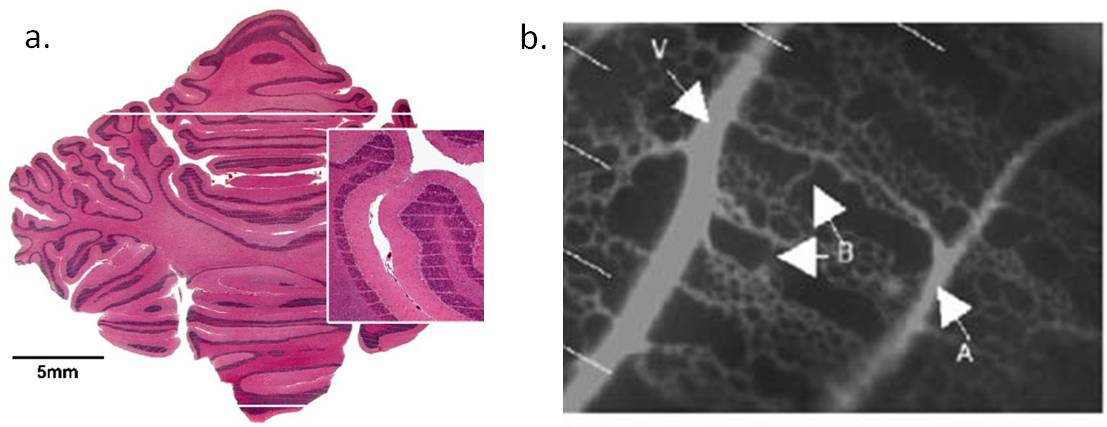
\includegraphics[width=\linewidth]{mrt_img/blattmann_mrt_hist}
	\caption{a. Horizontal section of the cerebellum of a piglet of 15 months after irradiation. Some cells and their nuclei directly in the path of microbeams were destroyed. There was no tissue destruction present, nor were there signs of haemorrhage. The paths of the microbeams appear in the section as thin, white horizontal parallel stripes,which are more easily visible in the insert. (Adapted from \cite{laissue2001weanling}.) b. CAM’s 24 h after irradiation, white lines indicate locations of microbeam planes, v = vein,  a = artery, b = bridge. Adapted from \cite{blattmann2005applications}. Both had skin entrance dose of 300 Gy, beam width 27 \si{\um} and beam separation 210 \si{\um}.}
	\label{fig:blattmann_mrt_hist}
	\end{figure}
	

	
	\subsubsection{Technical Challenges}
	%Technical challenges of MRT, delivery, synchrotron, MSC, dosimetry challenges, dosimetry needs: 2D& 3D
	
	
	The European Synchrotron Radiation Facility (ESRF) in Grenoble, France is pioneering MRT technology on the ID17 Biomedical beamline. Microbeam therapy must be delivered rapidly, in highly collimated beams to avoid spatial blurring of the beam due to patient movement. For this reason, the high-dose rates and minimal beam divergence of synchrotron radiation is ideal for MRT. Relatively low x-ray energies are used (20--100 keV) meaning penetration depth is limited and skin entrance doses are relatively large \cite{blattmann2005applications}. The healthy tissue-sparing geometry of MRT delivery compensates for this.
	
	
	MRT treatments are usually delivered as an array of highly collimated beams using a multi-slit collimator (MSC) \cite{brauer2005characterization}. The narrow microbeams (typically 50--100 \si{\um}) have large peak entrance doses, commonly over 100 Gy.
	The valley dose is made up of scattered radiation from surrounding beams and depends on the widths of the peak and valley areas, the depth and the total number of beams. The width of the valley area, the centre-to-centre (ctc) distance, is typically four times the width of the beam. 
	The geometry of irradiation has been shown to be important to the healthy tissue recovery. The valley dose must be sufficiently small and ctc distance sufficiently wide to allow repair of ablated regions in the peak area. However, to achieve good tumour control it is important to ablate enough tumour. Optimisation of MRT parameters is currently under way in a pre-clinical trial which is also assessing methods for treatment planning and accurate dosimetry for MRT. [REF]
	
	
	
	Commercial dosimetry systems are not appropriate for MRT due to the small beam size and high dose rates involved.	The small width of the microbeams means that traditional radiotherapy measurement devices (ion chambers, diode arrays, etc.) are inadequate. An ideal dosimeter for MRT would have micron-scale spatial resolution with a dynamic range of the order of 10,000.

    There are two competing measurement problems in modern MRT, which make it extremely challenging to devise a single technique for treatment verification and quality assurance (QA). Firstly, there is the need to characterise the individual microbeams and make accurate measurements of the peak-to-valley dose ratio (PVDR). The PVDR gives an indication of how safe and effective a treatment will be. A high PVDR, with a large peak dose and small valley between beams is desirable and this metric	depends on many factors including field size and depth. 

	The second problem is that, as MRT becomes increasingly sophisticated, there will be a need to provide high-quality 3-D dosimetry over the entire treated volume. Like conventional radiotherapy, MRT has developed complex delivery geometries including multi-port cross-firing \cite{brauer-krischnew2005} and interlacing \cite{brauer2013preclinical, serduc2009first,serduchigh-precision2010} (see Figure~\ref{fig:MRT_geometries}) in order to increase the dose at the tumour site, while sparing normal tissue. However, given the very small sizes of the beams in the case of MRT, a geometrical error of tens of microns could lead to a under- or over-dosing. Therefore, the delivery systems need to be accurate to sub-micron levels to avoid errors. %Despite the many advantages of MRT and our increasing ability to administer it safely, it is still extremely difficult to verify that the planned dose distribution has been accurately delivered. 
	Any uncertainty could complicate the interpretation of biological outcomes and may delay or limit clinical uptake, particularly in the paediatric patient populations for whom it could be especially suitable \cite{laissue2001weanling}.
		
	
\begin{figure}
\centering
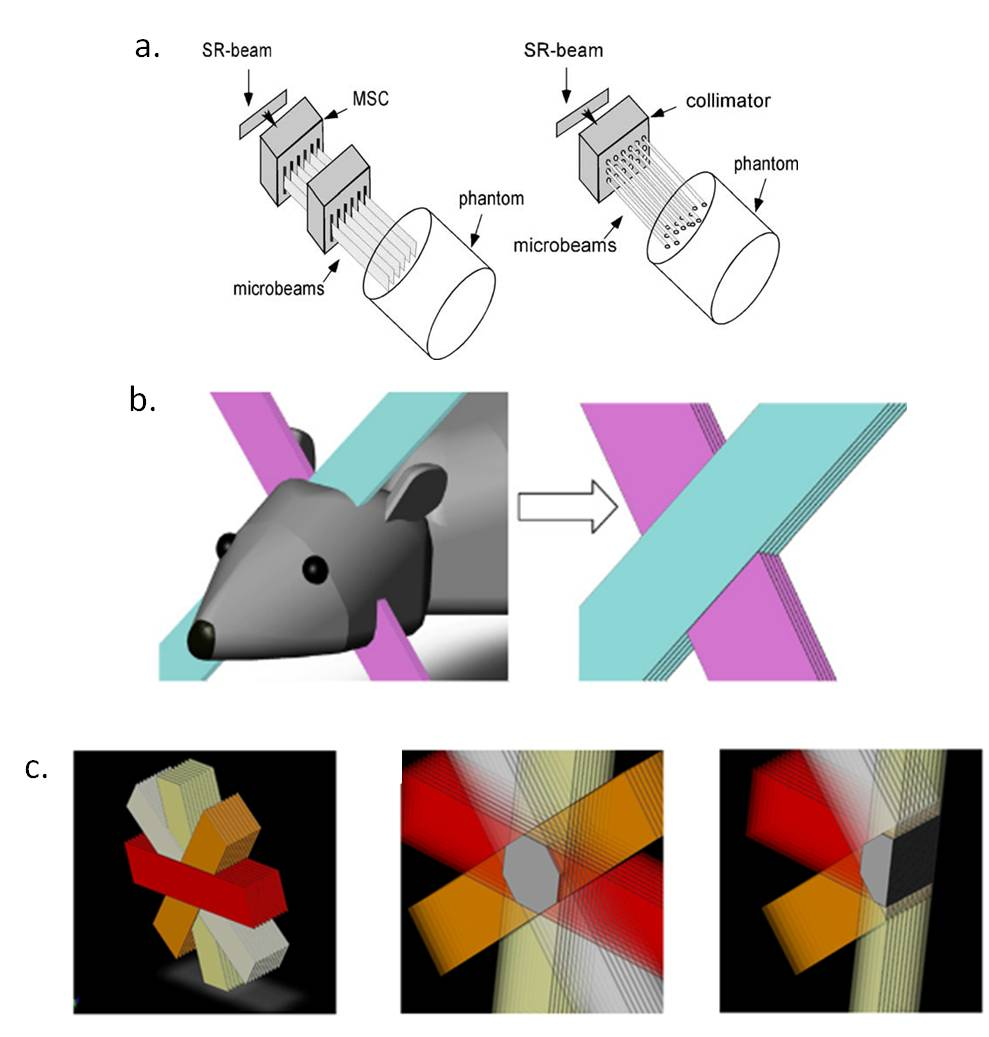
\includegraphics[width=0.8\linewidth]{mrt_img/MRT_geometries}
\caption{a. Pencil beams and planar b. cross-firing c. interlacing. Images adapted from \cite{siegbahndetermination2006}, \cite{brauer-krischnew2005}, \cite{serduchigh-precision2010} respectively.}
\label{fig:MRT_geometries}
\end{figure}
	
	It is the second requirement that we address in the current work. 
	A dosimeter is needed that can follow the entire `patient journey', with multiple repositioning steps, from the initial x-ray CT scan, through planning with the newly developed treatment planning system (TPS) to the final treatment. 
	
	
	\subsubsection{Dosimetry for MRT}
	%Dosimeters for MRT: current players
	
	As described by \cite{brauer-krischpotential2010}, there is a long history of investigating different techniques to obtain accurate dosimetry in this challenging situation. The devices evaluated include metal oxide-semiconductor field-effect transistors (MOSFETs) \cite{brauer2003mosfet, siegbahnmosfet2009}, fluorescent nuclear track detectors \cite{akselrod2006novel} and silicon strip detectors \cite{lerch2011dosimetry}.
	Previous studies have used thermoluminescent dosimeter (TLD) \cite{ptaszkiewicz2008tld} and radiochromic film (e.g., \cite{crosbie2008method, serduchigh-precision2010}) dosimetry to obtain 2-D information. Quantitative comparisons of film dosimetry and Monte Carlo models have shown good agreement, typically between 2 and 15\% depending on the exact measurement location \cite{martinez-roviradevelopment2012}.  However, whilst film is suitable for some applications (and particularly for the QA of individual fields), 2-D information is of limited use in complex 3-D treatments, such as those presented here. This argument also applies to the direct biological verification of treatment via histological sectioning. Although such work is indispensable for understanding the radiobiological effect of MRT \cite{crosbie2010tumor}, the quantity of data obtained and spatial coverage are often much more limited. Thus, it is of great interest to develop fully 3-D methods of quantitative, high-resolution dosimetry.
	
	Full 3-D dosimetry of radiosensitive samples has a long history. At the outset, the predominant readout modality was Magnetic Resonance Imaging (MRI) of radiochromic Fricke gels \cite{appleby1987imaging, schreiner2004review} or polymer gels \cite{baldock2010polymer,maryanski1993nmr}. The application of MRI dosimetry to MRT was investigated by (Dilmanian et al., 2008) but only for “thick microbeams” (680 \si{\um}) using a commercial scanner. \cite{berghigh2004}, \cite{bayrederthe2008} and \cite{heilemann2015pushing} have investigated the limits of MRI gel dosimetry for resolving small features, but the minimum width of irradiated region was 200 \si{\um}, a factor of four larger than the width of the microplanar beams studied here. The primary limitations for the MRI method are the r$^{–3}$ dependence of image signal-to-noise ratio (SNR) and the diffusion path length of water molecules during each scan step. A further problem is that the gels used cannot always support the high dose rates encountered in synchrotron MRT.
	
	\subsection{Optical CT dosimetry}
	%3D microdosimetry, MR insufficient, need for optical CT and PRESAGE
	%Description of PRESAGE, optical CT described in methods section but recap - differences of microsystem over other dosimetry applications
	
	Optical computed tomography (CT) \cite{doranthe2009, goreradiation1996}  is an alternative modality for 3-D dosimetry readout. Used for some time as a method of clinical verification in large dosimeters, the potential for optical CT using the radiochromic plastic PRESAGE\textregistered \ dosimeter in small-field imaging of millimetre-sized beams is now a subject of considerable interest \cite{clift2010toward}. Optical CT microscopy, also known as optical projection tomography (OPT), was first demonstrated in this context by \cite{doranan2010} and is an emerging modality that could fulfil the requirements for MRT dosimetry. It offers the exciting possibility of quantitative 3-D data with microscopic resolution, but over an extended field-of-view (FOV) within a macroscopic object. A recent study \cite{doranestablishing2013} performed a baseline assessment of the dosimetric accuracy of a microscopy system but highlighted that further improvements in resolution were necessary. To date, the highest nominal spatial resolution so far reported with PRESAGE\textregistered  \ is 78 nm, but those results were obtained using traditional fluorescent microscopy \cite{annabellevaluating2012} rather than transmission optical CT as here and, so far, only for 1-D patterns of dose deposition. %It is not yet clear whether that technique will scale up to 3-D over an extended field-of-view.
	More recently full 3-D imaging of fluorescence in PRESAGE\textregistered \ for MRT was demonstrated using confocal microscopy \cite{gagliardi2015high}. Add some comments.
	
	%In this article, we demonstrate the current capabilities and limitations of the optical CT system for the quantitative measurement of microbeams, and we present 3-D images of a range of complex MRT treatments. Given the prior experience of MRI described above, it was uncertain at the outset of our research whether such a 3D imaging technique would have sufficient resolution to image the microbeams at all, and obtaining truly quantitative data was an aspiration. However, as described below, the visualisation results were shown to be immediately useful in revealing discrepancies that might be attributable to mechanical issues during the dose delivery and the 3-D data show considerable potential for future developments of the method. Previous reports have shown a decrease in contrast when imaging small features with optical CT in what was thought to be a modulation transfer function (MTF)-related effect \cite{doranultra-high2013}. This raised the question of whether quantitative measurements of the microbeams themselves were possible with optical CT.
	
	The current work  has two aims. Section~\ref{sec:3dvis}: 3-D Visualisation establishes how PRESAGE\textregistered \ and optical CT can be used as a QA tool for MRT, fulfilling the 3-D dosimetry information gap. Section~\ref{sec:quantPVDR}: Quantitative measurements of PVDR, investigates in detail the reduction in contrast seen previously and assesses the extent to which optical CT can be used for PVDR measurement. 
	
	\subsubsection{PRESAGE\textregistered}
	
		PRESAGE\textregistered ~is a solid plastic radiochromic dosimeter  made of clear polyurethane combined with leucomalachite green. \cite{adamovics2003new} The optical density of the plastic changes after exposure to radiation making it very useful for monitoring 3-D dose delivery. PRESAGE\texttrademark ~has quite a high RI of around 1.5 which requires specialised matching liquid for imaging. 
		A  mix of  2-ethylhexylsalicylate (W514500-10KG-K, SigmaAldrich)
		%, RI %$n_{1} \approx 1.50$) 
		and 4-methoxycinnamic acid 2-ethylhexylester (Chem.   Art.   100255, Chemos GmbH) %, RI $n_{2} \approx 1.54$) 
		was made in an 11:1 ratio and then adjusted by trial and error to give a close match \cite{AbdulRahman:2011eqa}.
		To increase the dynamic range an oil-soluble green dye was added to give the liquid a similar absorbance as PRESAGE\textregistered.
		
		Custom-made PRESAGE\textregistered \ plastic dosimeters were supplied by the manufacturer (Heuris Pharma, Skillman, NJ). PRESAGE\textregistered \ is a solid, radiochromic 3-D dosimeter consisting of a transparent polyurethane matrix (approximately 90\% of the dosimeter by weight), 2\% leuco malachite green, and a 4\% trihalomethane initiator, with the remainder being a solubilizer for the dye and initiator. The PRESAGE® formulation used here has the stoichiometric chemical formula C$_{304}$H$_{510}$N$_{20}$O$_{71}$SBr, and a mass density of 1.11 gcm$^{-3}$.  The polyurethane leucodye solution was poured into a mould and pressurized at 60 psi for at least 48 hours to ensure a solid dosimeter. Samples were supplied in the form of cylinders of diameter 22 mm and 9.7 mm. These were machined to a uniform heights of 50 mm for the 9.7 mm diameter samples and 80 mm for the 22 mm diameter samples and inserted into a bespoke Perspex phantom that was used both for holding the samples and to provide adequate scatter conditions for secondary electronic equilibrium \cite{doranestablishing2013}.
			
		The linearity of the PRESAGE\textregistered \ dose response was confirmed using cuvettes irradiated with a range of doses and optical absorbance measured using a spectrophotometer (see Figure~\ref{fig:Presage_linearity}a\&b). The optical CT dose response for each batch of PRESAGE\textregistered \ was measured with specially designed calibration samples containing squares of a range of doses. The linear dose response was confirmed and these samples allow a dose-pixel value conversion for different depths in PRESAGE\textregistered \ (see Figure~\ref{fig:Presage_linearity}c--e).
		
		
		\begin{figure}
			\centering
			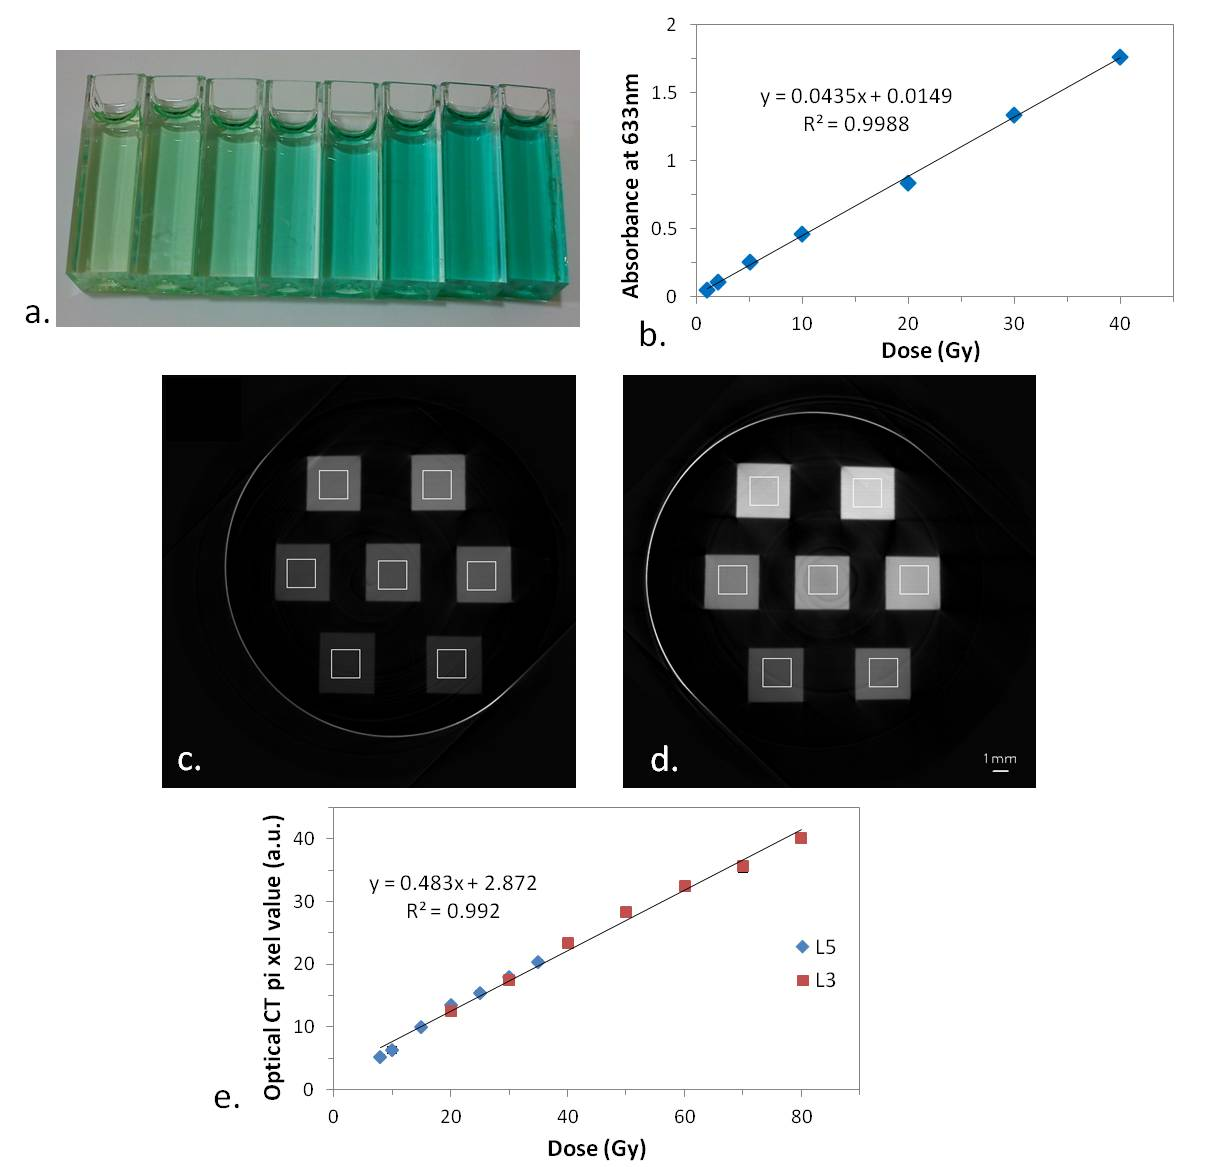
\includegraphics[width=\linewidth]{mrt_img/Presage_linearity}
			\caption{a. Cuvettes of PRESAGE irradiated with the RMH linac with a range of doses, b. the optical absorbance of the cuvettes measured using a spectrophotometer. c. sample L5 with dose calibration pattern and d. sample L3 with higher doses, both at depth of 0.3 cm e. the calibration curve for the two samples at depth of 0.3 cm. }
			\label{fig:Presage_linearity}
		\end{figure}
		
		%as matching liquid.   Based on an estimate of the PRESAGE\texttrademark ~RI, n, supplied by the manufacturer, a calculation was made via the approximate formula
		%  \begin{equation}
		%  n = f n_{1} + (1 - f )n_{2}  
		%\end{equation}
		
		%where $n$ is the RI of PRESAGE\texttrademark ~and $f$ is the volume fraction of salicylate. An initial mixing ratio of around 11:1 was  
	
	Aims for these experiments: evaluate optical CT as dosimetry method that could be used in clinical trials of MRT.
	
	\section{3-D Visualisation}
	\label{sec:3dvis}
	\subsection{Methods and Materials}
	
	
	\subsubsection{Sample irradiation}
	Irradiations were carried out at the European Synchrotron Radiation Facility (ESRF) in Grenoble, on the ID17 biomedical beamline. The methodology, equipment and beam characteristics have already been described in detail \cite{abdulrahmansophisticated2011 , doranestablishing2013 , doranan2010} and, here, the additional information relates only to the specifics of the MRT irradiations delivered. 
	
	Successful delivery of MRT dose patterns is extremely demanding from an engineering point of view. Accurate sample alignment plays a key role and a 3-D dosimeter capable of a simple `hit-or-miss' assessment is highly desirable. The pattern formed by the 2-D intersection of multiple, angled arrays of microbeams has the potential to be extremely complicated and so the use of a single or small number of 2-D films for QA purposes is not a viable option. Furthermore, performing accurate quantitative measurements of 2-D optical density on multiple films is an extremely time-consuming operation. Having a method of generating information to correct or improve the MRT delivery would be extremely useful. For this purpose, fully quantitative measurements of peak dose would not be required. Instead the main requirements are fast readout, ease of use, spatial accuracy and visualisation of dose integration. 
	
	To test whether optical CT is suitable in this capacity, different complex MRT irradiations were performed, listed in Table~\ref{table:samples}. These included collimated beams (pencil beams, sample 1.1) \cite{brauer-krischeffects2010}, interlacing of microplanar beams (multiport and offset, sample 1.2) \cite{serduchigh-precision2010}, multi-port cross-firing of microplanar beams with the use of an anthropomorphic head phantom (sample 1.3, see Figure~\ref{fig:Fig1christopher}) \cite{requardt2005new}. All beams had a full width half maximum (FWHM) of 50 \si{\um} and centre-to-centre (ctc) spacing of 400 \si{\um} between beams.
	
	\begin{table}[H]
		\centering
		\begin{tabular}{ p{1.4cm} | p{3cm} |p{1cm} | p{2cm} |p{6.5cm}  }
			%\hline
			\textbf{Sample} & \textbf{Irradiation type} &\textbf{Peak dose (Gy)}   &\textbf{Dosimeter size (mm)} & \textbf{Description} \\ \hline
			1.1  & Pencil beams & 300  & 9.7 & Four fields of $7\times 7$ interlaced circularly collimated `pencil' beams, separated by  \ang{45} rotation. \\ \hline
			1.2  & Interlacing & 200  & 9.7 & Four $(5\times 5)$mm$^2$ microplanar arrays separated by \ang{45} rotation and 200 \si{\um} offset. \\ \hline
			1.3  & Multiport crossfiring & 200  & 22 & In anthropomorphic head phantom, three $(10\times 10)$mm$^2$ microplanar arrays separated by \ang{60} rotation. \\ \hline
			2.1  & Single microplanar array & 100  & 9.7 & $(10\times 10)$mm$^2$ microplanar array field. \\ \hline
			2.2  & Single microplanar array & 50  & 9.7 & $(10\times 10)$mm$^2$ microplanar array field. \\ \hline
			2.3  & Single microplanar array & 100  & 9.7 & $(30\times 30)$mm$^2$ microplanar array field. \\ %\hline
		\end{tabular}
		\caption{List of sample irradiations.}
		\label{table:samples}
	\end{table}
	
	
	\subsubsection{Optical CT microscopy}
	Imaging was performed using the optical CT microscope described in \ref{sec:opticalCTmeth}. With the previously reported system (\cite{doranestablishing2013})it took approximately 1 hour 10 minutes to acquire the data for a $512^3$ voxel reconstructed volume. The equivalent scan takes under 3 minutes with the new system, making optical CT a viable system for \emph{in situ} feedback for MRT irradiations. Although, for the results presented here, the scanner and irradiation facility were not co-located, there is clear potential for installing an optical CT microscope in the beamline `hutch' of the accelerator. The new automated positioning system and custom-made sample mounts allows reproducible sample scanning position, making it easy to measure the samples immediately pre- and post-irradiation, thus potentially allowing absolute measurements of optical density change in the future, reducing artefacts and baseline uncertainties. 

	Two scanning procedures were used for scanning dosimetry samples, detailed in Table~\ref{table:scansettings}. Samples $1.1−1.3$ were scanned using a `fast' three minute scan of 1000 projections over \ang{180} rotation, each of $512 \times 512$ pixels, satisfying the Nyquist condition for the reconstruction of an isotropic data volume of $512^3$ voxels. The FOV was (13.3 mm)$^3$ for the 9.7 mm diameter samples (1.1 and 1.2) and (26.6 mm)$^3$ for the 22 mm diameter sample (1.3) with isotropic reconstructed voxel sizes of (26 \si{\um})$^3$ and (52 \si{\um})$^3$ respectively.
	
	\begin{figure}
		\centering
		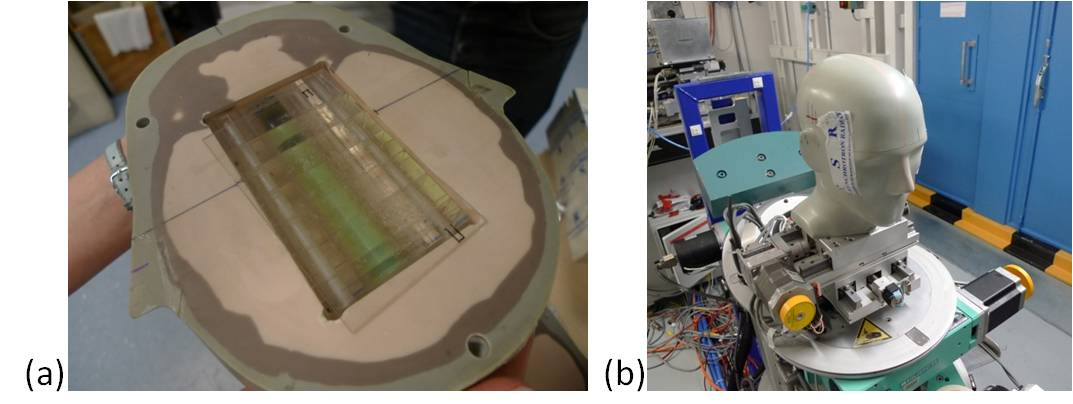
\includegraphics[width=0.9\linewidth]{mrt_img/mrt_Fig1}
		\caption{(a) PRESAGE\textregistered \ sample 1.3 in place in anthropomorphic head phantom and (b) the head phantom being positioned for irradiation at the ESRF.}
		\label{fig:Fig1christopher}
	\end{figure}
	

	
	
	Optical CT imaging of PRESAGE samples was carried out in two modes.
	For qualitative visualisation of irradiation patterns fast scans were used, while samples for PVDR assessment were scanned with high-resolution scans. All scans had an aperture setting of A1 so that the DOF encompassed the entire sample.
	
	
	
	\begin{table}[H]
		\centering
		\begin{tabular}{ p{2.3cm}  p{2.5cm} p{2.5cm}  p{2.3cm} p{2.5cm}  }
			\hline
			\textbf{Scan} & \textbf{Projections} &\textbf{Pixels}   &\textbf{Voxel size (\si{\um})} & \textbf{Acquisition time} \\ \hline 
			Fast  & 1000 & $512\times 512$  & 20.8 & 2.5 minutes \\ %\hline
			High-resolution & 3200 & $2048\times 256$ &  5.2 & 1 hour \\ 
			\hline
		\end{tabular}
		\caption{Different scanning parameters for MRT}
		\label{table:scansettings}
	\end{table}
	
	
	
	
	\subsection{Results}
	High quality image datasets were acquired for each sample and the microbeams are easily visualised. The reconstructed 3-D datasets can be visualised in different ways to provide an assessment of the irradiation. Figure~\ref{fig:Fig2MIP} shows a maximum intensity projection (MIP) image of a reconstructed image volume of sample 1.1, with the full dataset available in movie format as online supplementary material. This type of visualisation is very powerful, allowing the user to assess quickly that the pencil beam irradiation has been delivered successfully and is well centred within the sample. Confirming this would be very difficult using 2-D dosimeters. 
	
	\begin{figure}
		\centering
		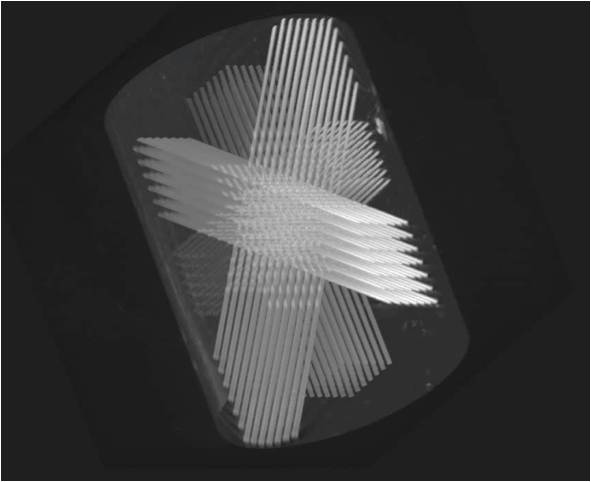
\includegraphics[width=0.7\linewidth]{mrt_img/mrt_Fig2}
		\caption{A maximum intensity projection (MIP) image of sample 1.1 showing excellent visualisation of the microbeams, confirming successful irradiation which was well centred within the sample. Full 3-D reconstruction can be seen in a supplementary video.}
		\label{fig:Fig2MIP}
	\end{figure}
	
	
	Figure~\ref{fig:Fig3S9} shows a reconstructed slice through sample 1.2, irradiated with an interlaced dose pattern. More views are available in supplementary video material. It is clear that interlacing of the centre and left fields was successful. However, the centre and right fields are overlapping and the increased dose is visualised as a brighter region on optical CT images. This demonstrates the qualitative dose integration visualisation power of optical CT, which would be very helpful during MRT set-up even without a quantitative measure of the increased dose. This visualisation could inform on patient safety and would be complicated to measure with a 2-D dosimeter. 
	
	\begin{figure}
		\centering
		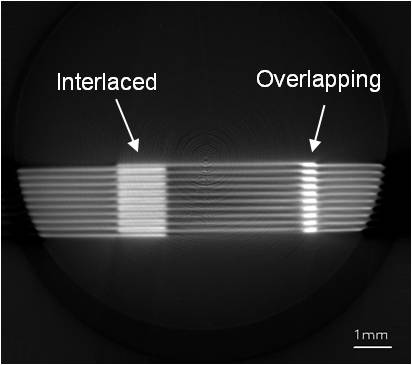
\includegraphics[width=0.7\linewidth]{mrt_img/mrt_Fig3}
		\caption{A reconstructed slice through sample 1.2 with an interlaced dose pattern which has overlapped, leading to overdosing compared to the expected treatment. Further slices from the full dataset are available in a supplementary video.}
		\label{fig:Fig3S9}
	\end{figure}
	
	
	Figure~\ref{fig:Fig4L7} shows two orthogonal reconstructed slices through sample 1.3 which was irradiated inside an anthropomorphic head phantom with a multi-port cross-firing geometry. With the ability to choose the image plane arbitrarily, it is easy to find a slice that gives direct interpretation of the delivered dose, unlike the image shown in Figure~\ref{fig:Fig4L7}(a). The second image, shown in Figure~\ref{fig:Fig4L7}(b), clearly shows that two of the delivered fields are off-centre and a simple measurement the offset could be used to correct the MRT geometry (red arrow). This interpretation would be very difficult from a 2-D measurement as the 2-D dosimeter would need to be placed very accurately. 
	
	
	\begin{figure}
		\centering
		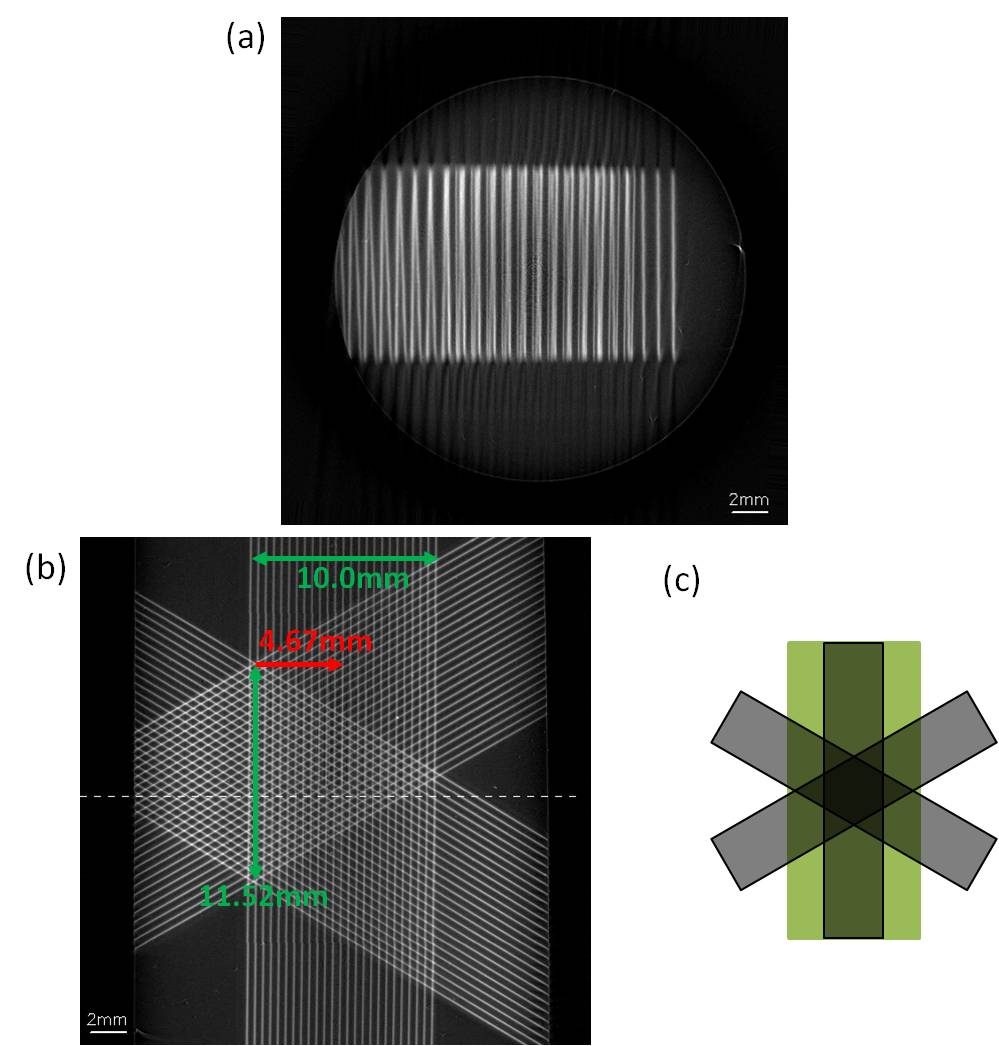
\includegraphics[width=0.9\linewidth]{mrt_img/mrt_Fig4}
		\caption{(a) A reconstructed slice through sample 1.3 which was irradiated inside an anthropomorphic head phantom with a multiport cross-firing geometry. From this view it is difficult to tell whether the irradiation was successful. (b) A reconstructed slice in the orthogonal plane, with the z position of (a) marked by the dotted line. Green arrows mark field measurements which are as expected, showing that three irradiations have been delivered at the expected field size and spaced \ang{60} apart as expected. However, two of the fields are offset from the centre of the sample, (c) shows the expected shape of the irradiation. The red arrow denotes the offset of the two incorrect fields from the centre of the sample, this measurement could be used to correct the MRT geometry.}
		\label{fig:Fig4L7}
	\end{figure}
	
	
	
	
	\section{Quantitative measurements of PVDR}
	\label{sec:quantPVDR}
	
	Previously reported decrease in contrast with small features - can we quantitatively measure microbeams and PVDR? Why we want to, possible problems.
	
	\subsection{PVDR measurement}
	PRESAGE\textregistered \ samples were irradiated with microplanar arrays of different field sizes and different peak doses to provide a range of PVDRs for comparison with Monte Carlo and film data. Samples were laid in the phantom and exposed end-on to a single irradiation from a multi-slit collimator of slit width 50 \si{\um}, centre-to-centre spacing 400 \si{\um} \cite{brauer2009new}. Two 9.7 mm diameter samples were exposed with a nominal peak dose to the surface of the dosimeter of 50 Gy and 100 Gy, both with a field size of $(10 \times 10)$ mm$^2$ (samples 2.1 and 2.2 respectively). A third 9.7 mm sample was exposed with a nominal peak dose of 100 Gy, with field size ($30 \times 30$) mm$^2$ (sample 2.3, see Table~\ref{table:samples}). 
	
	Samples 2.1−-2.3 were scanned using a `high-resolution' scan consisting of 3300 projections, each averaged over five acquisitions of 2048 $\times$ 256 pixels, reconstructed to a data volume of 2048 $\times$ 2048 $\times$ 256 voxels with FOV (10 $\times$ 10 $\times$ 1.25) mm. Using the full matrix size of the new camera across the width of the sample allows significantly higher sampling frequency over previous reports, with an isotropic reconstructed voxel size of (5.2 \si{\um})$^3$. A smaller matrix height of 256 pixels was chosen for reduced acquisition and reconstruction times. The large computer RAM of 256 GB allows readout of the large amounts of data simultaneously making these scans a manageable 1 hour long. The projections were acquired with the largest DOF setting (smallest NA, setting A1), reflecting the `ideal' focal situation of constant resolution across the entire sample. The samples were scanned at depths of 0.3 cm, 1 cm and 4 cm for comparison with Monte Carlo and film measurements of PVDR \cite{martinez-roviradevelopment2012}. 
	
	
	\subsection{Sampling investigation}
	Description of code...

	
	\subsection{Deconvolution}
	Using a high NA would give a high resolution at the cost of a small DOF, resulting in out-of-focus data being superimposed on top of in-focus data requiring deconvolution. To investigate whether the resolution could be improved through deconvolution with a measured point-spread-function (PSF), a PSF phantom was designed. The PSF phantom was made using 1 \si{\um} diameter beads (56314, Sigma-Aldrich) which were suspended in 0.75\% agarose gel. The gel was dehydrated in 100\% ethanol and then soaked in matching fluid (97\% ethyl hexyl salicylate and 3\% 4-methoxycinnamic acid 2-ethylhexyl ester) giving the same refractive index as the PRESAGE\textregistered. Superglue was used to attach the bead phantom to the end of PRESAGE\textregistered \ sample 2.1. The bead phantom was then included in the FOV during a `high-resolution' scan consisting of 3300 projections, each averaged over five acquisitions of 2048 $\times$ 256 pixels, reconstructed to a data volume of 2048 $\times$ 2048 $\times$ 256 voxels with FOV (10 $\times$ 10 $\times$ 1.25) mm. The lens aperture was set to A4  which had the largest DOF for 10 \si{\um} resolution (see Table~\ref{table:DOFNA}). 
	
	When images were reconstructed, in principle a bead at point (x, y, z) has experienced the same optical blur as at point (x, y, z + $\Delta $z). Assuming this, a bead in the centre of the sample in good focus was used as a PSF during Richardson-Lucy deconvolution of the microbeam profile axially above it at a depth of 0.3 cm in PRESAGE\textregistered. Deconvolution was performed in the IDL software environment (Exelis Visual Information Solutions, Boulder, CO) using the `deconv' tool \cite{varosi1993idl}, assuming Poisson noise. The PVDR from the resulting deconvolved profile was calculated for different numbers of deconvolution iterations.
	
	\subsection{Results}

	
	\subsubsection{PVDR measurement} 
	Figures~\ref{fig:Fig7}a\&b show a reconstructed optical CT image of PRESAGE\textregistered \ sample 2.1 and the associated profile through the marked position on the image. To reduce noise, profiles were median-averaged in the two orthogonal directions to the microbeam variation resulting in an effective pixel size of 104 \si{\um} in those directions and 5.2 \si{\um} across the profile. Over this small distance there is no divergence of the peak pixel position in the orthogonal directions as the beam divergence is very small. 
	
	As no part of the sample was unirradiated, the baseline corresponding to zero-dose pixel value used is an average of values obtained from unirradiated areas of other samples from the same batch, hence the large uncertainty marked on the graph. In future a pre-scan can reduce this error. As can be seen the sampling frequency is very high, however the beams appear blurred compared to the shape observed with other higher-resolution modalities. 
	
	The PVDR was calculated for sample 2.1 at depths of 0.3 cm, 1 cm and 4 cm. Samples 2.2 and 2.3 were also measured at a depth of 4 cm. The results of the optical CT PVDR measurements are plotted against the expected values from Monte Carlo simulation \cite{martinez-roviradevelopment2012} in Figure~\ref{fig:Fig7}c, where the large error-bars on the optical CT measurements are principally due to the baseline uncertainty. Encouragingly, the variation of PVDR with depth and field size corresponds extremely well between optical CT and Monte Carlo measurements with a very high correlation coefficient for the linear fit. However, the absolute value of the PVDR, as measured by optical CT is consistently only 30\% of the expected value. There could be several reasons for this. Given that decreasing the peak entrance dose has no effect (sample 2.2) it is unlikely to be due to a lack of dynamic range in the optical CT scanner. Sample 2.3 has a larger field size and therefore larger valley dose. Given that this measurement also fits the trend it is unlikely that low SNR in the valley measurement is the primary source of the error. 
	
	The full-width half-maximum (FWHM) of one of the beams in Figure ~\ref{fig:Fig7}b is 62.4 \si{\um}, not 50 \si{\um} as expected. This implies that the profile is blurred, which would reduce the peak value measured. Although the nominal pixel size is 5.2 \si{\um}, the true resolution is lower than this, limited by the imaging optics, as expected from our MTF measurements. 
	
	The results of knife-edge measurements of the MTF over an extended DOF are shown in Figure~\ref{fig:MTFDOF}. These results show that with NA setting A1, the ideal situation of a constant resolution across the entire FOV is broadly achieved. However, the maximum resolution is only $21.5 \pm 0.5$ \si{\um}. A resolution of 10 \si{\um} is achieved when the NA is increased at an aperture setting of A4, but in this case, the DOF less than 0.6 mm (see Table~\ref{table:DOFNA}).
	
	\begin{figure}
		\centering
		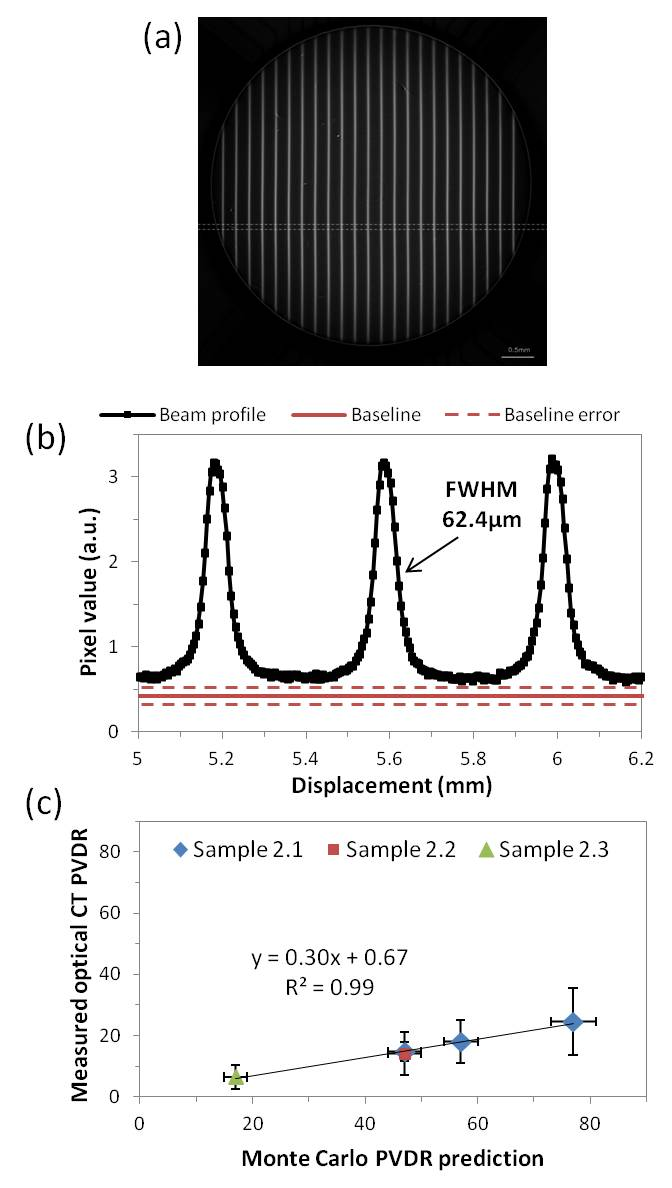
\includegraphics[width=0.6\linewidth]{mrt_img/mrt_Fig7}
		\caption{(a) Reconstructed image of sample 2.1 and (b) the corresponding profile through microbeams. The baseline is an average value from unirradiated areas on other samples from the same batch, hence the large uncertainty. The profile was median averaged along 20 pixels in the directions orthogonal to the profile to improve the SNR resulting in 5.2 \si{\um} pixel size across the profile and 104 \si{\um} pixel size in the orthogonal directions. (c) Comparison of PVDR measurements using optical CT against expected values from Monte Carlo simulation \cite{martinez-roviradevelopment2012}.}
		\label{fig:Fig7}
	\end{figure}
	
	\subsection{Sampling investigation}
	In a basic simulation of our system, we found that to measure the peak of a Monte Carlo-simulated 50 \si{\um} microbeam with an error of less than 1\%, a sampling resolution of 10 \si{\um} is required. Therefore, the optimum NA giving this resolution over the largest DOF needs to be found.  
		
		\begin{figure}
			\centering
			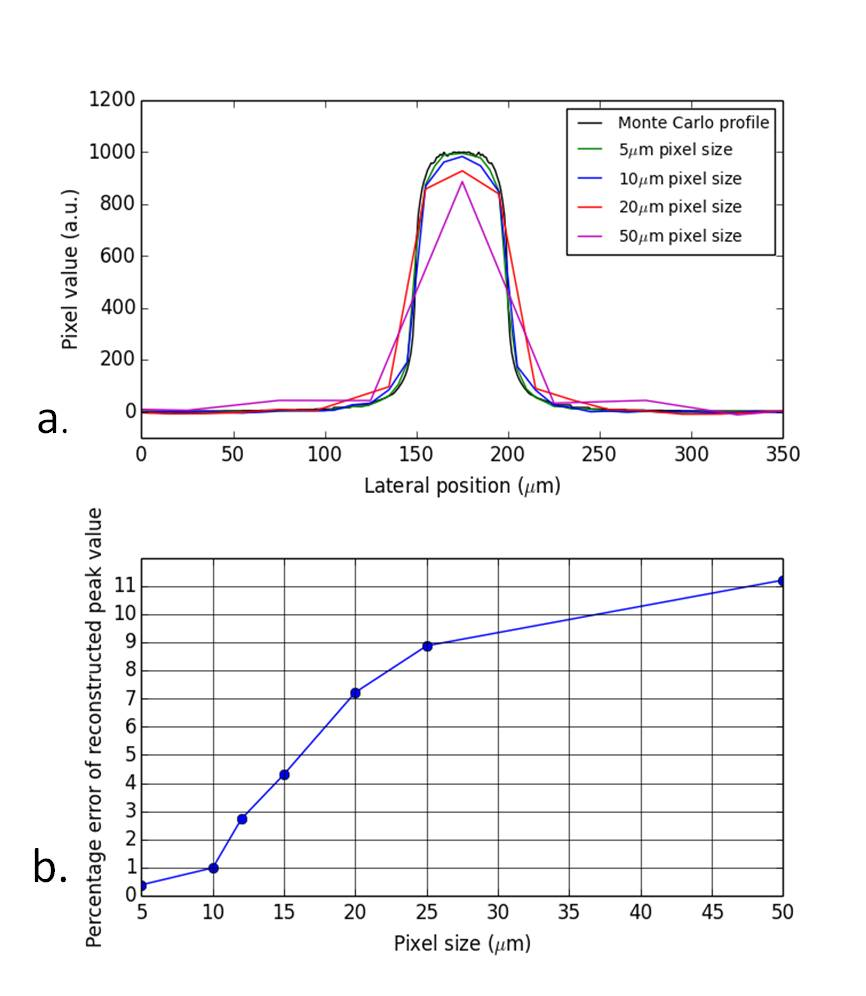
\includegraphics[width=0.8\linewidth]{mrt_img/Beam_10um_sampling}
			\caption{Simple simulation of sampling MC MRT beam with different pixel sizes}
			\label{fig:Beam_10um_sampling}
		\end{figure}
	
	\subsubsection{Deconvolution}
	Figure~\ref{fig:Fig8}a shows a microbeam profile and its improved shape after deconvolution with a PSF measured using a 1 \si{\um} diameter bead. However, Figure~\ref{fig:Fig8}b clearly demonstrates that although the deconvolution improves the shape of the profile, the PVDR measured is dependent on the number of deconvolution iterations performed, and does not converge before the noise reaches an unacceptable level. This means that this type of deconvolution approach is not reliable enough to use in quantitative measurements of PVDR of microbeams. This may also apply to depth-of-field scanning techniques previously employed in biological imaging to improve the resolution \cite{fauverthree-dimensional2005}. 
	
	\begin{figure}
		\centering
		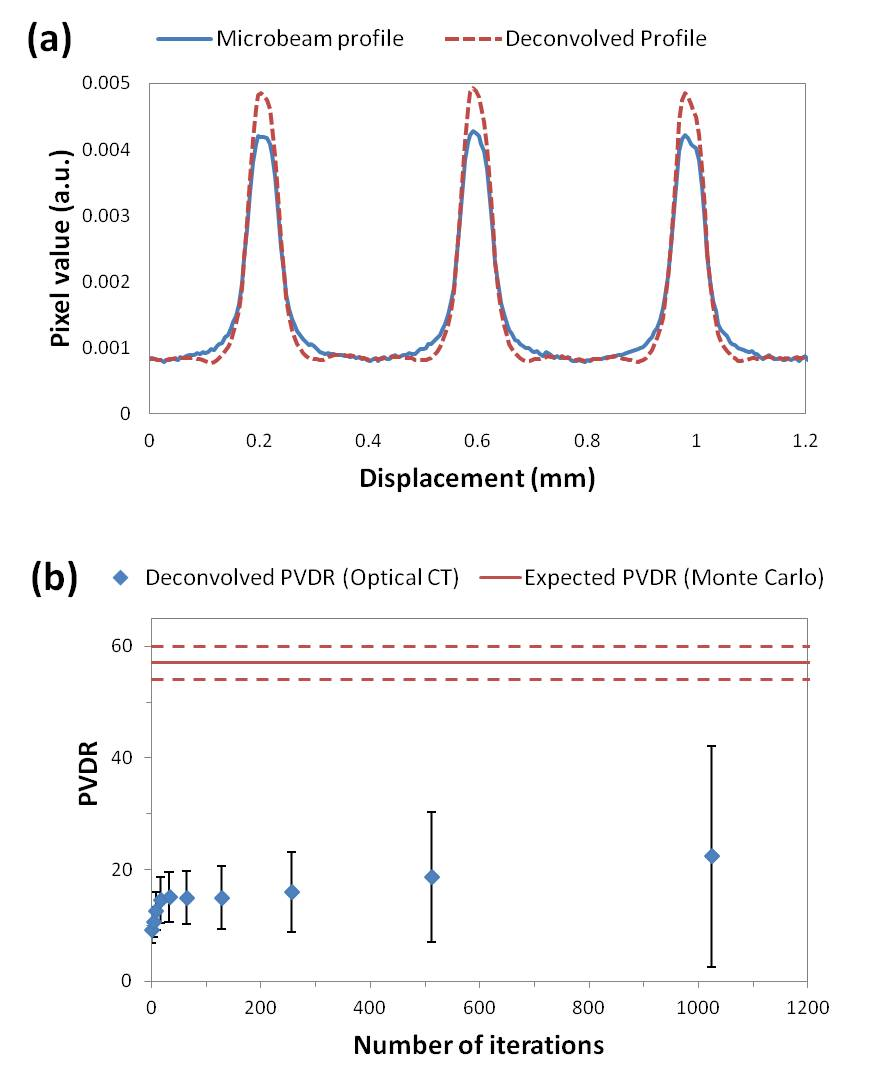
\includegraphics[width=0.85\linewidth]{mrt_img/mrt_Fig8}
		\caption{a. A microbeam profile from sample 2.1 and the deconvolved profile after 4 iterations of Richardson-Lucy deconvolution using a PSF calculated from a 1 \si{\um} bead. This shows that deconvolution of the PSF improves the shape of the profile however, b. shows that the PVDR depends on the number of deconvolution iterations, which does not appear to converge before becoming extremely noisy. Therefore although deconvolution can qualitatively improve the images, we are hesitant to base any quantitative measurements on a deconvolved profile.}
		\label{fig:Fig8}
	\end{figure}
	
	
	\section{Discussion}
	Section~\ref{sec:3dvis} clearly suggests that optical CT has the potential to play an important role in MRT QA. The data of Figures~\ref{fig:Fig2MIP}--\ref{fig:Fig4L7}, rendered in 3-D in the accompanying movies, demonstrate graphically where the real benefit of the optical CT technique lies. Image data may be acquired from the entirety of the sample at high resolution in a single measurement. This would be very useful for hit-or-miss assessment and imaging is now fast enough to provide correction information to improve MRT irradiations \textit{in situ}. Compared with a single, or small number of 2-D film images, there are no difficulties in interpreting the measured dose distribution in multiport treatments. Using the solid PRESAGE\textregistered \ dosimeter also allows for end-to-end QA of the entire treatment process including CT scan, treatment planning, positioning and delivery which would be necessary before MRT is translated to clinical use. One potential future application would be to combine PRESAGE\textregistered \ dosimetry with a patient motion simulating platform which can investigate whether very complex irradiations such as interlacing are possible with patient breathing motion. 
	
	The time between irradiation and readout was longer than desirable, during which time the samples were refrigerated. The potential time-evolution of the measured doses is discussed in \cite{doranestablishing2013} but whilst the error introduced at this step is expected to be significant, the pertinent observation for the purposes of this work is that PRESAGE\textregistered \ exhibits negligible diffusion of the dose-reporting chromophore. Thus, blurring of the microbeam dose due to the delay is not expected to have occurred.
	
	The apparatus is sufficiently compact that a copy could be installed in the MRT hutch at ID-17. A number of improvements to the imaging methodology would be possible if the apparatus were located in situ at the beamline:
	\begin{itemize}
		\item As was discussed in \cite{doranestablishing2013}, pre-scanning the dosimeter would enable effects of refraction to be largely eliminated and an accurate zero-dose baseline to be established, for absolute measurements of valley dose given the new accurate positioning system.
		\item Images could be acquired within minutes of the end of the irradiation, eliminating any uncertainties caused by delayed readout, for example, related to time-evolution of the PRESAGE\textregistered \ dose-response \cite{skyttemperature2011 , skyttemperature2012}.   
		\item Further improvements in image SNR and extensions to the dynamic range of acquired data would be achievable via the acquisition of multiple datasets with different levels of illumination \cite{krstajiccharacterization2007 , thomasa2011}.
	\end{itemize}
	
	
	The results of Section~\ref{sec:quantPVDR} suggest that accurate PVDR measurements are not possible with the current optical CT arrangement. Given the results of the knife-edge measurements of MTF along the optical axis, we believe the underestimation of the PVDR by optical CT is primarily due to lack of true spatial resolution. Attempts to improve the resolution by increasing the numerical aperture and deconvolution using a measured PSF lead to unreliable and noisy results, making these methods unsuitable for clinical measurements of PVDR.   
	
	It remains an open question as to whether the optical CT technique will in future prove capable of making measurements of PVDR that are competitive with other methods such as those employing 2-D TLD films or MOSFET detectors. There are two possible avenues to move forward with quantitative microbeam measurements using optical CT. 
	
	First, using a smaller sample would mean that both the necessary FOV and DOF can be decreased, making it possible to increase the magnification and resolution. Although this involves the sacrifice of spatial information across the beams, full depth information would still be retained. This would enable, among other things, measurement of the effects of scattering along the entire length of the microbeams, rather than simply at a single depth determined by the detector location. 
	
	Second, while the measured resolution of $21.5 \pm 0.5$ \si{\um} in projections with NA setting A1 is insufficient for sampling the peak dose, it should be sufficient for quantitatively measuring the valley dose, which is four times wider than the peak. Arguably, in terms of patient safety the valley dose is the most important factor, as once the peak is over a certain value, cell death will occur. Therefore, having a valley measurement in 3-D, in combination with an alternative 2-D measurement of the peak dose on entry, could be of significant interest to the MRT community.
	
	\section{Conclusions}
	3-D images of geometrically sophisticated synchrotron microbeam therapy deliveries have been obtained. The most significant current limitation of the imaging technique as presented here is the available spatial resolution, which has been investigated in detail. Although the data presented here fall some way short of the dose quantification needed for complete verification, the measurements and visualisations have already demonstrated their utility by detecting deviations from a planned treatment (Figures~\ref{fig:Fig3S9}, \ref{fig:Fig4L7}(b)) and shown clear potential for quantitative measurement of the biologically important valley dose.
	
	
	
	
	

	\chapter{Spleen}
	
	\section{Introduction}
	
	
	
	
	Toxicity is an important consideration in drug development and off-target effects are common, with potentially significant adverse side-effects. Methods that provide informative, accurate and rapid assessment of drug-induced toxicity to major target organs, such as the liver, kidneys and spleen, can either positively impact and accelerate the development of promising new agents, or force early closure of a programme that ultimately will not deliver a safe drug. They also inform design of subsequent clinical trials, ensuring imaging protocols are optimised to include potentially critical normal tissues.
	
	
	In the treatment of cancer, a number of agents designed to specifically target the tumour vasculature have been and continue to be developed. Given the hypervascular nature of the spleen, its essential role as a blood filter and the unique presence of acute endothelial contractility \cite{raganspontaneous1988}, the effects of these vascular targeting agents on splenic perfusion are also commonly assessed. Typically, this has been achieved pre-clinically through the use of histological markers of perfused vasculature or tissue uptake of radiolabelled blood flow tracers. \cite{cullistumour2006, horsmanvascular2003} Splenic perfusion has also been assessed as part of clinical trials of vascular targeting agents by incorporating functional imaging, where the spleen is included in the imaging field-of-view (FOV). \cite{andersonassessment2003, evelhochmagnetic2004} 
	
	The spleen has a complex 3-D structure made up of several distinct tissue types. Extensive interconnections between red pulp, white pulp and intermediary marginal zones are integral to the organ's function. \cite{groomthe1987} Traditional 2-D histology methods are not well suited for the examination of these 3-D features and they are often subject to sampling error due to the limitations of the physical sectioning techniques used. In addition, it is time-consuming to match information between adjacent slices, which may be distorted by the histological preparation process. A number of imaging approaches have been applied to the spleen, including microvascular-corrosion casting, scanning and transmission electron microscopy (SEM, TEM), and in vivo microscopy. \cite{groomthe1987}  These can have excellent resolution, but are often complex to perform and expensive.
	
	Optical computed tomography (CT) is an emerging imaging modality. Although initially introduced in 1996 to solve problems in the physical sciences \cite{goreradiation1996, winfreequantitative1996}, the first micro-imaging measurements on tissue were presented somewhat later, in 2002, using the Optical Projection Tomography (OPT) variant of the scanner geometry. \cite{sharpeoptical2002} This technique has subsequently been applied to the imaging of whole rodent organs and embryos in a variety of contexts. \cite{oldhamthree-dimensional2007, sharpeoptical2003}  The FOV size sits in the ``imaging gap'' between confocal microscopy and magnetic resonance imaging (MRI), ranging from a single cell to several centimetres, with resolution generally proportional to the FOV.
	
	Prior to optical CT imaging, tissue samples must, in general, undergo a process of optical clearing to render them transparent at optical wavelengths. \cite{oldhamoptical2008, zhurecent2013}  Optical CT images can be acquired in absorption or fluorescence modes, and the contrast observed can be either endogenous (related to the remnant optical absorption of tissue after the clearing process, or the tissue autofluorescence), or exogenous in the form of optical stains which are well characterised in the field of histopathology. Previously OPT has been used to probe developing spleens in embryos \cite{asayeshspleen2006, hecksher2004splanchnic}, but the technique has not been applied to adult mouse spleen in which the 3-D features are fully developed.
	
	In this study, the ability of endogenous optical CT contrast to detect and to assess quantitatively the microstructure of normal adult murine spleen was investigated. In addition, structural changes were also characterised in spleens excised from mice following treatment with the vascular disrupting agent (VDA) ZD6126. A previous 2-D assessment, using fluorescence microscopy of Hoechst 33342 uptake \cite{cullistumour2006}, demonstrated a significant reduction in splenic perfusion with this agent, making it a highly relevant case study.
	
	\section{Materials and Methods}
	
	\subsection{Tissue collection}
	ZD6126 (N-acetylcolchinol-O-phosphate, Angiogene Pharmaceuticals Ltd.) was formulated in 20\% of 5\% sodium carbonate and 80\% phosphate-buffered saline (PBS). 
	All in vivo experiments were performed in accordance with the local ethical review panel, the UK Home Office Animals (Scientific Procedures) Act 1986, the United Kingdom National Cancer Research Institute guidelines for the welfare of animals in cancer research \cite{workman2010guidelines} and the ARRIVE (animal research: reporting in vivo experiments) guidelines \cite{mcgrath2010guidelines}. Six-week-old female Balb/c mice were randomised to be treated with either vehicle alone (n=3) or 200mg/kg ZD6126 i.p. (n=3). The small sample size was chosen to minimise animal use in this initial proof-of-concept study. No adverse effects were observed in any mice and after 24 hours the mice were killed by cervical dislocation and the spleens excised and placed in 70\% ethanol in PBS overnight at $4^{\circ}$C.
	
	\subsection{Optical CT imaging}
	Spleens were first embedded in 0.75\% agarose (Sigma-Aldrich, Gillingham, UK) and kept in 70\% ethanol in PBS overnight at room temperature. The samples were then dehydrated with three washes of 100\% ethanol over three days. Optical clearing was achieved with a graded series of ethanol and 1:2 benzyl benzoate:benzyl alcohol (BABB) solutions (Sigma-Aldrich, Gillingham, UK), with washes of 30\% and 70\% 1:2 BABB in ethanol, each for one day, followed by two washes of 100\% 1:2 BABB over a one week period. 
	
	Imaging was performed using an in-house optical CT system, shown in Figure~\ref{fig:1}, which was previously developed and well characterised for microbeam radiotherapy applications. \cite{doranestablishing2013} Optical CT image reconstruction is similar to x-ray CT in that a series of `projection' images are acquired, recording photon attenuation at different angles. Each sample was suspended from a sample holder and rotated $180^{\circ}$ from above in a matching tank containing 1:2 BABB fluid, which has the same refractive index as the optically cleared samples. In order to achieve high resolution, a microscope zoom lens (Z16 APO zoom system, Leica Microsystems GmbH, Wetzlar, Germany) was used to focus each projection image onto a complementary metal-oxide semiconductor (CMOS) camera (Zyla sCMOS, Andor Technology PLC, Belfast, UK). Filtered backprojection was used to reconstruct axial slices through each sample from the many 2-D projection images. 
	
	Two datasets were acquired for each optically cleared spleen, each based on a raw dataset of 1000 projection images of $512\times 512$ pixels, acquired over $180^{\circ}$ rotation and reconstructed to a $512^3$-voxel volume. Dataset 1 had a FOV of (13.3 mm)$^3$ and isotropic voxels of size (26 $\mu$m)$^3$, while Dataset 2 had a FOV of (5.3 mm)$^3$ and isotropic voxels of size (10.4 $\mu$m)$^3$. 
	
	\begin{figure}%[H]
		\centering
		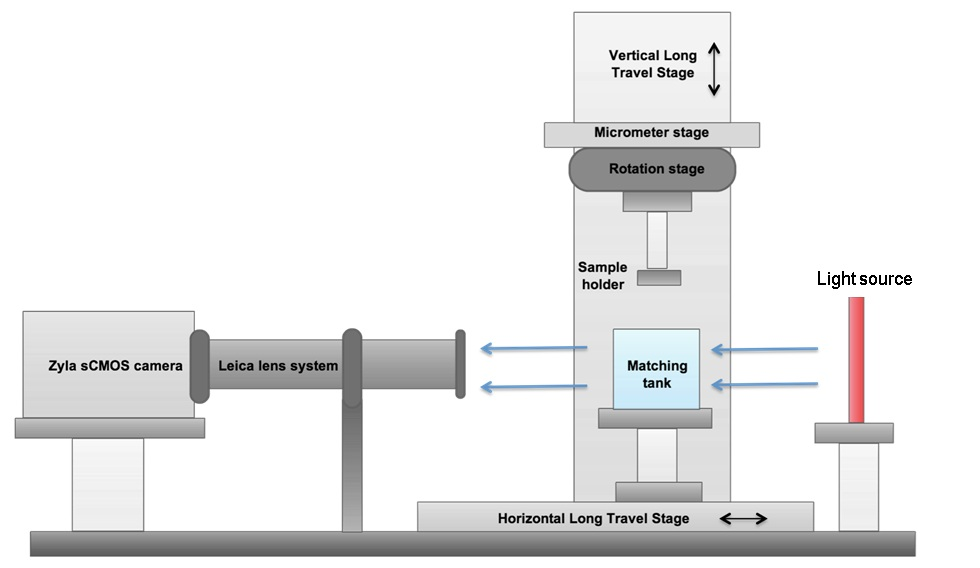
\includegraphics[width=0.8\textwidth]{spleen_img/spleen_Figure1.jpg}
		\caption{Diagram of the optical CT system used for imaging optically cleared spleen samples. Light passing through the sample was focused by a microscope lens system onto a camera chip and recorded in a projection image for each rotation angle. See \cite{doranestablishing2013} for details of individual components.}
		\label{fig:1}
	\end{figure}
	
	
	The first scan encompassed the entire spleen height, enabling accurate total volume measurements. The second scan had a reduced FOV to enable acquisition of higher resolution data over a limited height, providing more detailed images of the internal tissue structure. Dataset 1 was acquired using a wavelength of 630nm (Flat-panel LEDR, Phlox, Aix-en-Provence, France). For increased contrast between the red and white pulp regions, a wavelength of 430nm was chosen for Dataset 2 (SugarCUBE\texttrademark LED Illuminator, Nathaniel Group Inc. Vergennes, VT, USA and 430/10nm bandpass filter, Thorlabs Inc., Newton, NJ, USA), which is near the peak absorption wavelength of deoxyhaemoglobin and also strongly absorbed by oxyhaemoglobin.
	
	
	
	\subsection{Image Analysis}
	Volume measurements were carried out by segmenting spleen from background in each slice and counting the total number of spleen voxels. Segmentation was done in OsiriX. \cite{rossetosirix:2004}  For each sample, images were imported as a stack of image files in JPEG format and the spleen was outlined manually every 20 axial slices. Using the `Generate Missing ROIs' tool in OsiriX, outlines were interpolated for the other slices. Each slice was visually inspected to ensure accuracy with some minor adjustments made where necessary. The total volume of the outlined regions was calculated using OsiriX given the known voxel volume of (26 $\mu$m)$^3$. This method is advantageous over threshold-based segmentation as highly attenuating artefacts were excluded. The volume results for each cohort were tested for significant difference using a non-parametric one-tailed Mann-Whitney U test at the 95\% confidence limit.
	
	Quantitative analysis of internal structures was performed by comparing various textural statistics between samples. Due to the irregular size and shapes of the spleens, regions-of-interest (ROIs) of size $200 \times 200 \times 30$ pixels in similar positions were analysed for each sample, as shown in Figure~\ref{fig:2}. 
	
	The grey-level co-occurrence matrix (GLCM) is a standard method of calculating textural features in 2-D images. \cite{haralicktextural1973} ROI voxel values were scaled from 32-bit to 8-bit integers, and image contrast was enhanced via histogram equalisation for each sample ROI. The 2-D GLCM size scales with the square of the number of image grey levels. A GLCM for an 8-bit image has 216 elements, compared to 264 elements for a 32-bit image, which is on the order of exabytes. Therefore, scaling to 8-bit is customary to give a tractable computation time, 75 minutes in our case using a Dell PC with 256GB RAM. Additionally, it was found that a linear scaling of optical CT image intensity to grey-level value suppressed image contrast due to the presence of some highly attenuating artefacts. Histogram equalisation was therefore employed to maintain intra-sample contrast despite sacrificing inter-sample comparability of absolute values. This process can amplify noise, so a median filter with a kernel width of 3 was applied prior to analysis to improve the signal-to-noise ratio (SNR). This width was chosen given the interest in long-range textural features, such as red and white pulp boundaries that change over larger pixel distances.
	
	Standard 2-D GLCMs were calculated for each 2-D $x-y$ slice in the sample ROIs for a range of pixel displacements and averaged over four angular directions ($\theta = 0^{\circ}, 45^{\circ}, 90^{\circ}, 135^{\circ}$, see Figure~\ref{fig:2}). \cite{haralicktextural1973} However, to take into account the 3-D nature of the data, the GLCM analysis was extended to include a third reference point in the $z$ direction, giving rise to a 3-D GLCM (see Figure~\ref{fig:2}d). The 3-D GLCM, $P_{d,\theta}$ for an $n \times m \times p$ image volume, $I$, is defined below (Equation~\ref{eqn2}) where $d$ is the pixel displacement and $\theta$ is the displacement angle, related to pixel position changes $\Delta x, \Delta y$  and $\Delta z$  as follows,   
	
	\begin{equation} \label{eqn1}
	\Delta x = \Delta z = d \cos \theta , \quad \Delta y = d \sin \theta
	\end{equation}                        
	
	\begin{equation}\label{eqn2}
	P_{d,\theta}(i,j,k)= \sum_{x=0}^{n-1} \sum_{y=0}^{m-1} \sum_{z=0}^{p-1} \begin{cases} 1, &\mbox{if } 
	\begin{array}{l} 
	I(x,y,z)=i \\
	I(x+\Delta x,y +\Delta y,z)=j \\
	I(x,y+\Delta y,z+\Delta z)=k 
	\end{array} \\
	0, & \mbox{otherwise}  \end{cases}
	\end{equation}
	
	3-D matrices were calculated for a range of d values and averaged over four angular directions ($\theta = 0^{\circ}, 45^{\circ}, 90^{\circ}, 135^{\circ}$). Contrast and homogeneity were calculated from these 3-D GLCMs according to equations adapted from \cite{cheniris2009} (see Equations~\ref{eqn3} and \ref{eqn4} where $N_g$ is the total number of grey levels). The analysis was not blinded and these endpoints were decided after data acquisition.
	
	\begin{equation}\label{eqn3}
	Contrast = \sum_{i,j,k=0}^{N_g-1} P_{i,j,k}[(i-j)^2+(i-k)^2+(j-k)^2]
	\end{equation}
	
	\begin{equation}\label{eqn4}
	Homogeneity = \sum_{i,j,k=0}^{N_g-1} \frac{P_{i,j,k}}{1+(i-j)^2+(i-k)^2+(j-k)^2}
	\end{equation}
	
	\subsection{Simulation}
	In order to investigate some of the variables affecting the textural metrics above we performed 2-D GLCM analysis on simple simulations of a single spleen slices, incorporating three different tissue types present within the spleen. At the chosen imaging wavelength of 430nm, a strong source of optical absorption is haemoglobin in red blood cells (RBCs). The red pulp areas of the spleen transport and trap some RBCs making these areas highly absorbing on our optical CT scans. White pulp areas including lymph nodes do not usually contain RBCs and are therefore far less absorbing. The marginal zone between red and white pulp can trap RBCs to a lesser extent than the red pulp giving it intermediate absorption. 
	
	Simulated spleen images were generated incorporating these three tissue types. Each simulated image had four `features' made up of a simulated  lymph node and surrounding simulated marginal zone. The lymph nodes were simulated as circles, with constant grey level value of 0. The marginal zone was represented as a circular disc around the lymph node with uniform grey level value of 128 and the surrounding areas simulated the red pulp, with a grey level value of 256. Four simulated spleen images were generated with different lymph node and marginal zone radii, changing the total size of the features and the ratio of marginal zone area within each feature. 2-D contrast was calculated for each case.
	
	
	\begin{figure}%[H]
		\centering
		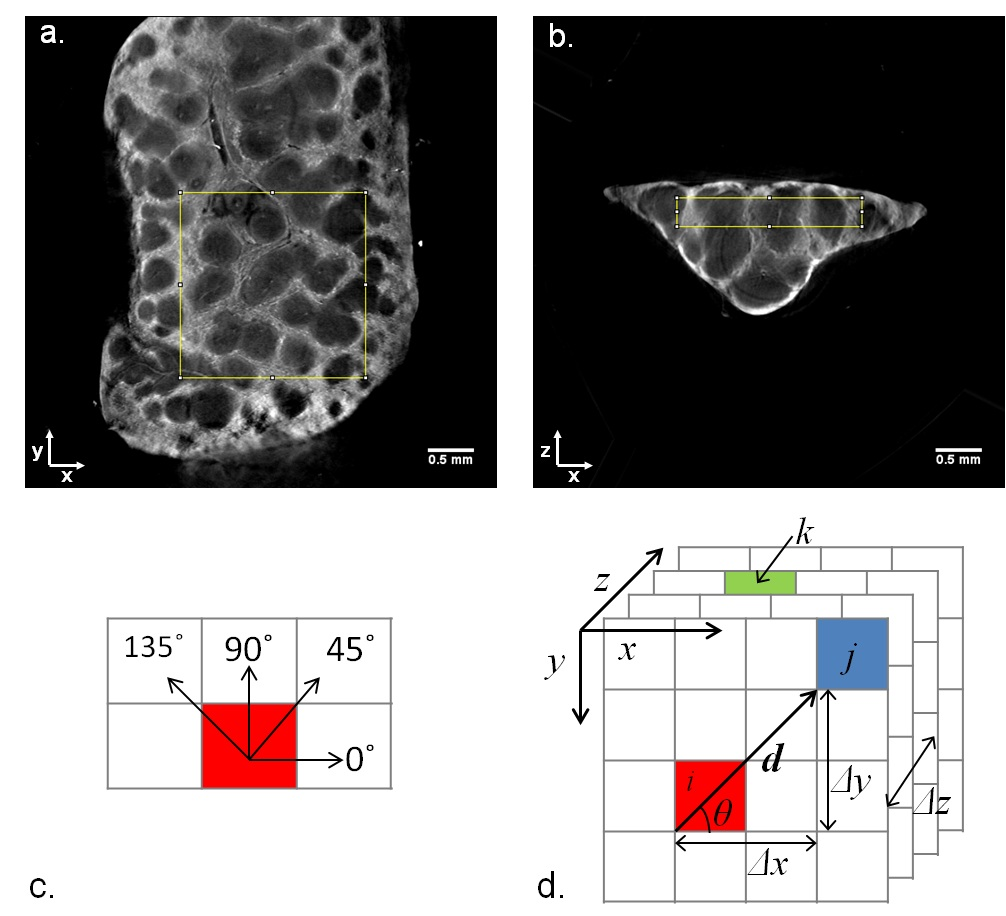
\includegraphics[width=0.8\textwidth]{spleen_img/spleen_Figure2.jpg}
		\caption{a. and b. Orthogonal cross-section slices of a reconstructed ZD6126-treated spleen image volume from Dataset 2 with FOV (5.3 mm)$^3$. The yellow boxes indicate the position of the region-of-interest (ROI) (size $200 \times 200 \times 30$ pixels) chosen for textural feature analysis. ROIs for the other samples were chosen to be in similar positions with respect to spleen boundaries. c. Representation of the four angular pixel directions used in grey level co-occurrence matrix (GLCM) calculations. For each pixel displacement, $d$, GLCMs were calculated in each angular direction and averaged to give one GLCM per displacement distance. d. Demonstration of the relative positions of three reference pixels used in 3-D GLCM calculations for the case of $d = 2$ and $\theta=45^{\circ}$. For 2-D GLCM calculations only pixels $i$ and $j$ were compared. 3-D GLCM analysis incorporates depth information by including a third reference pixel, $k$, in the $z$ direction. Pixel positions changes  $\Delta x, \Delta y$  and $\Delta z$  can be calculated from Equation~\ref{eqn1}.}
		\label{fig:2}
	\end{figure}
	
	
	
	
	
	\section{Results}
	High contrast data were successfully acquired for each spleen, and all animals were included in analysis. Figures~\ref{fig:3}a. and \ref{fig:3}b. display typical examples of the 3-D image datasets, in two complementary representations revealing the classical honeycomb appearance and complex inner structure. Full 3-D representations are available as supplementary video files. Figure~\ref{fig:3}c. shows a single 2-D reconstructed slice annotated to show some anatomical features. 
	
	The total volume of each spleen is plotted in Figure~\ref{fig:3}d. where there is a significant difference between the ZD6126-treated and vehicle groups. Total splenic volumes in the vehicle group ranged from $57.4\text{mm}^3 − 63.9\text{mm}^3$, while the ZD6126-treated group volumes ranged from $40.6\text{mm}^3 − 45.8\text{mm}^3$ demonstrating a ZD6126-induced median shrinkage of 28\% with significance of $\text{p}=0.05$.
	
	\begin{figure}%[H]
		\centering
		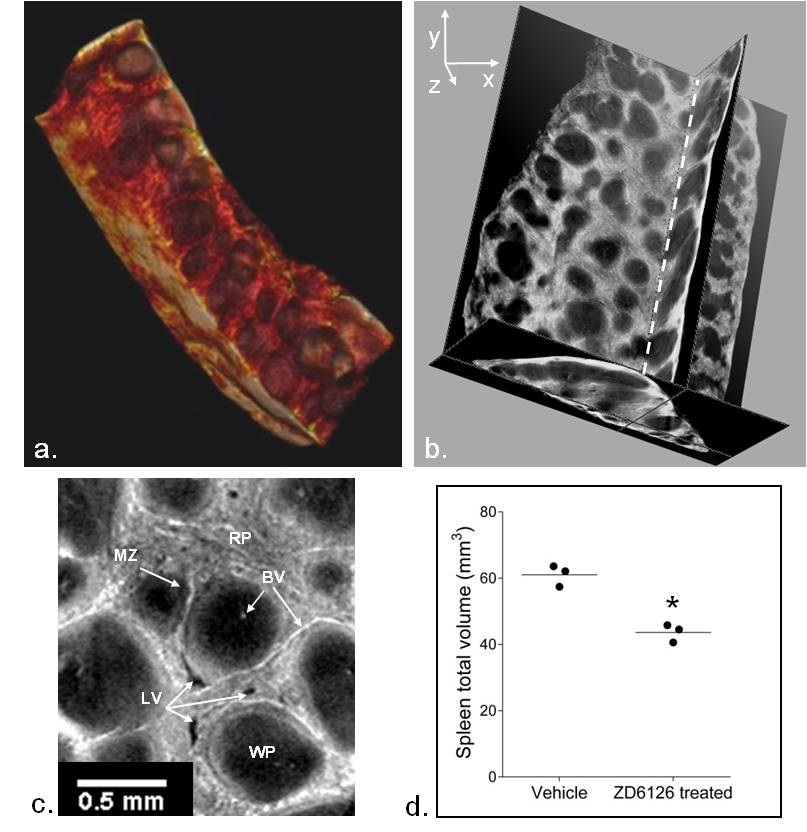
\includegraphics[width=0.8\textwidth]{spleen_img/spleen_Figure3.jpg}
		\caption{a. A still image from a volume rendering of a ZD6126-treated spleen from Dataset 2 with FOV (5.3 mm)$^3$, rendering made using OsiriX software. \cite{rossetosirix:2004}  b. A still view of orthogonal slices through a reconstructed volume of another ZD6126-treated spleen with FOV (5.3 mm)$^3$.  Full representations of these datasets are available online as video clips. c. A magnified view of a single slice from the volume shown in b., with some anatomical features marked. RP: red pulp, MZ: marginal zone, BV: blood vessel, LV: lymph vessel, WP: white pulp. Note that blood is highly attenuating and appears bright on these scans. d. Total volume of vehicle and ZD6126-treated spleens (lines mark the mean for each group, *$\text{p}=0.05$).}
		\label{fig:3}
	\end{figure}
	
	
	\begin{figure}%[H]
		\centering
		
\includegraphics[width=0.8\textwidth]{spleen_img/spleen_Figure4.jpg}
		\caption{The calculated 2-D contrast parameter for two different 2-D slices from each sample region-of-interest, after histogram equalisation and median filtering, for a range of pixel displacements. The solid lines show the mean values for each group. It is evident that separation of ZD6126-treated and vehicle cohorts depends on the slices compared, the groups are distinct for almost all length scales in slice 1 (a.) but overlap for the majority of pixel displacements in slice 30 (b.). }
		\label{fig:4}
	\end{figure}
	
	
	Our initial 2-D GLCM analysis, calculated as specified by (Haralick and Shanmugam, 1973), 
	was found to be slice-dependent (Figure~\ref{fig:4}). However, the modified GLCM analysis incorporating three reference points (equation~\ref{eqn2}) reduced the influence of analysis position on results. Calculation of the 3-D contrast and homogeneity texture parameters defined in equations~\ref{eqn3} and \ref{eqn4} showed a clear separation between ZD6126-treated and vehicle groups as shown in Figures~\ref{fig:5}b and c. The position of peak contrast was shifted to smaller pixel displacements for the ZD6126-treated samples with a peak contrast occurring at a distance of $18.2 \pm 0.9$ pixels for ZD6126-treated samples and $20.2 \pm 0.9$ pixels for the vehicle cohort, representing a physical difference of $20.8\mu m$.
	
	After analysis of 2-D simulations of splenic features it was found that features with smaller radii resulted peak contrast occurring at smaller pixel displacements and simulations with decreased marginal zone area had increased 2-D contrast (Figure~\ref{fig:6}). 
	
	\begin{figure}%[H]
		\centering
		\includegraphics[width=0.8\textwidth]{spleen_img/spleen_Figure5.png}
		\caption{a. Example 2-D slices from each sample region-of-interest after histogram equalisation and median filtering. ZD6126-treated spleens (T1−3) demonstrate visibly sharper boundaries between regions than vehicle spleens (V1−3). b. 3-D contrast, and c. 3-D homogeneity for each sample, for different pixel displacements (average of four angles $0^{\circ}, 45^{\circ}, 90^{\circ}, 135^{\circ}$). The solid lines show the mean values for each group at each pixel displacement and there is a clear separation between the groups for a range of pixel displacements. This gives an indication of the length scales of the features that are different between the groups.}
		\label{fig:5}
	\end{figure}
	
	\begin{figure}%[H]
		\centering
		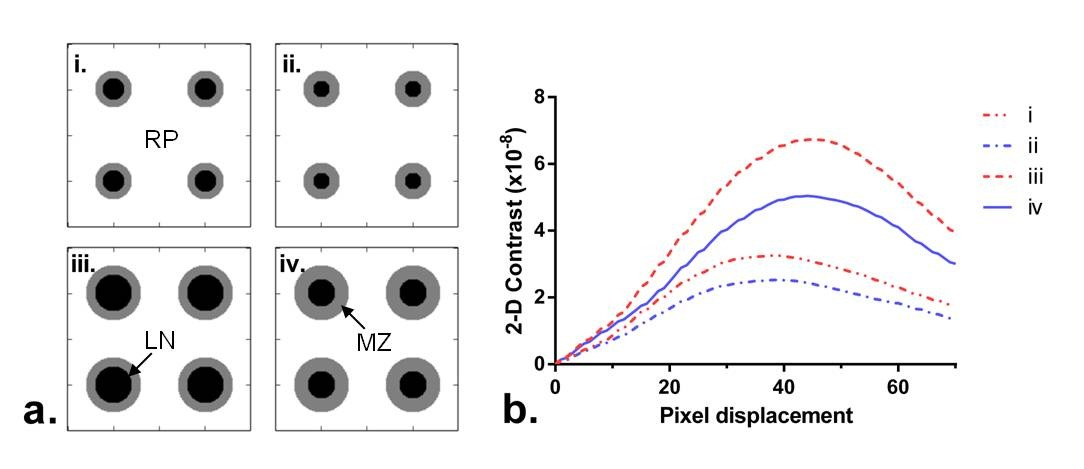
\includegraphics[width=0.8\textwidth]{spleen_img/spleen_Figure6.jpg}
		\caption{a. Simple simulations of spleen features, RP: red pulp, LN: lymph node, MZ: marginal zone. The overall feature size was varied (i and ii had smaller features than iii and iv), as was the area of MZ in each feature (increased MZ area in samples ii and iv compared to i and iii respectively). b. 2-D contrast for each simulation, i−iv, for a range of pixel displacements. The peak contrast for simulations i and ii was shifted to smaller pixel displacements compared to iii and iv. Decreased MZ area resulted in higher 2-D contrast.}
		\label{fig:6}
	\end{figure}
	
	
	
	\section{Discussion}
	In this study, we were able to demonstrate the use of endogenous optical CT contrast to provide distinct images of murine spleen microstructure, and its sensitivity to treatment-induced effects on spleen function following administration of the VDA ZD6126. Differences in spleen structure between the two groups were clearly observed via optical CT and changes in total spleen volume, 3-D contrast and homogeneity were determined.
	
	Owing to the distortions induced by physical sectioning of the samples and the other difficulties described in the introduction, assessment of volume is problematic using standard 2-D histology techniques. Thus, the volume difference between ZD6126-treated and vehicle spleens may not have been detected using conventional histology due to the irregularity of spleen shapes. The changes in volume observed in our optical CT images may not be linearly related to actual changes in vivo due to the nature of the clearing process. Dehydration causes tissue shrinkage and the amount of shrinkage may depend on original tissue size and density. Nevertheless, given our observations and the results of previous studies using ZD6126 and another VDA, AVE8062 \cite{cullistumour2006, guffroyevaluation2004}, it is highly likely that the drug has caused the spleen to contract. This is thought to be a consequence of the sensitivity of the atypical sinusoidal, unstable endothelium of the spleen \cite{groomthe1987} to tubulin-binding VDAs. 
	
	As shown in Figure~\ref{fig:4}, 2-D GLCM statistics gave different results depending on the slice analysed. This is because the complex 3-D structure of the spleen cannot truly be sampled in one slice, emphasising the need for 3-D analysis. 
	
	Direct biological interpretation of textural feature statistics is difficult given that many factors contribute to the final result. Qualitatively we noticed that the ZD6126-treated samples appeared to have a steeper gradient of grey values between white and red pulp areas (Figure~\ref{fig:5}a). The results of the simple simulation (Figure~\ref{fig:6}) suggest that the higher 3-D contrast of ZD6126-treated spleens at certain pixel displacements could be related to contraction of the marginal zone area leading to apparently sharper definition of the red pulp, supported by the observed difference in volume. This is also consistent with the shift in 3-D contrast peak position to smaller pixel displacement for the ZD6126-treated group, which supports the hypothesis that internal structures are smaller on average in the ZD6126-treated group.
	
	In previous findings, ZD6126 was found to reduce spleen perfusion, associated with red pulp areas as measured by uptake of Hoechst 33342. \cite{cullistumour2006} The reason for the reduction in mean Hoechst perfused area observed may be due to a contraction of the overall marginal zone and red pulp volume. However, this hypothesis is likely to be difficult to test, as the process of staining with Hoechst 33342 involves frozen sections which is currently incompatible with optical CT tissue preparation steps. 
	
	\section{Conclusion} 
	The effects of the VDA ZD6126 on the spleen were detected and characterised in 3-D, using an optical CT anatomical scan sensitive to haemoglobin absorption contrast. In the future this could be extended using optical stains providing additional functional information. For example, India ink would provide detail of perfused vessels and fluorescent micro-particles can indicate the degree of RBC trapping in the red pulp and marginal zones of the spleen. Indeed, there are plenty of data from these initial scans that could be extracted with further computational analysis.
	
	We have shown that spleen imaging using optical CT is potentially a very useful measure of spleen structure in 3-D, complementary to ultra-high resolution 2-D methods such as SEM and TEM. This method can be more straightforward than microvascular-corrosion cast methods, which involve many more preparatory steps prior to imaging and can be susceptible to practical problems in delivering resin down to the capillary level. Further investigation is continuing, including testing different functional stains and characterising the effect of the clearing process on this contractile organ. The promising results of this proof-of-concept study suggest a useful role for optical CT in assessment of drug-induced changes. Future studies with a larger cohort to enable robust statistical testing, will establish the significance of the quantitative changes and the sensitivity of the technique. 
	

	\chapter{Vasculature Imaging}

\subsection{Vascular staining}

\subsubsection{India Ink}

\begin{figure}
	\centering
	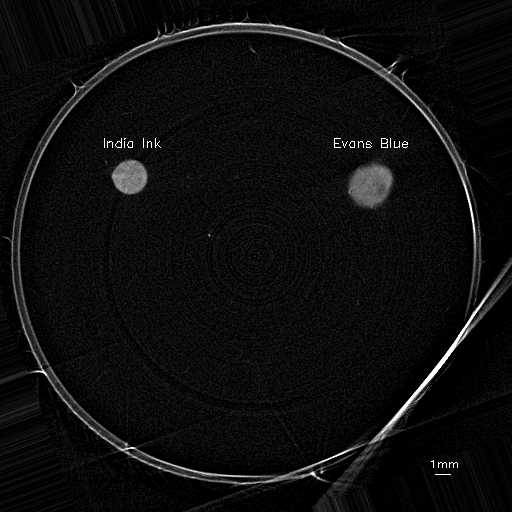
\includegraphics[width = 0.46\textwidth]{meth_img/3_EB_Ink_2mm_slice400_btscled.png}
	\caption{Phantoms with fingers containing Evans Blue, India Ink and clear gelatin.}
	\label{subfig:phant5}
\end{figure}




Figure shows that India Ink doesn't diffusive - good for staying in vessels. But Evans blue does - useful as a permeability marker.
	\chapter{Conclusions}
This shows...

	
	% A glossary and list of acronyms may go here
	% or may go in the front matter after the abstract.
	% The bibliography will go here
	\bibliography{thesis_bib}
\end{document}